\def\BookRunningTitle{A New Proof of an Arithmetical Theorem}
\documentclass[11pt,oneside,openany]{book}
\usepackage[paperwidth=6.5in,paperheight=9.5in,inner=0.72in,outer=0.72in,top=0.75in,bottom=0.78in,headheight=14pt]{geometry}
\usepackage{fix-cm}
\usepackage{fontspec}
\setmainfont{lmroman10-regular.otf}[BoldFont=lmroman10-bold.otf,ItalicFont=lmroman10-italic.otf,BoldItalicFont=lmroman10-bolditalic.otf,SmallCapsFont=lmromancaps10-regular.otf]
\usepackage{amsmath,amssymb,graphicx,array,microtype,fancyhdr,needspace}
\usepackage{longtable}
\usepackage[unicode,hidelinks]{hyperref}
\hypersetup{pdftitle={Carl Friedrich Gauss: Werke, Band II},pdfauthor={Carl Friedrich Gauss}}
\setlength{\parindent}{1.2em}
\setlength{\parskip}{0pt plus .3pt}
\setlength{\emergencystretch}{1.4em}
\pagestyle{fancy}\fancyhf{}
\fancyhead[L]{\small\nouppercase{\BookRunningTitle}}
\fancyfoot[C]{\thepage}
\renewcommand{\headrulewidth}{.25pt}
\newcommand{\SourceLeaf}[1]{\hypertarget{native-#1}{}\label{native-#1}}
\newcommand{\Article}[1]{\par\medskip\Needspace{4\baselineskip}\pdfbookmark[1]{Art. #1}{paper-one-art-#1}\centerline{\textbf{#1.}}\nobreak\smallskip}
\newcommand{\BookRule}[1]{\par\smallskip\centerline{\rule{#1}{.35pt}}\smallskip}
\newcommand{\dotsfour}{\mathinner{.\,.\,.\,.}}
\newcommand{\dotstwo}{\mathinner{.\,.}}
\newcommand{\dotsfive}{\mathinner{.\,.\,.\,.\,.}}
\newcommand{\pdot}{\mathbin{.}}
\newcommand{\gbr}[1]{\left[#1\right]}
\widowpenalty=10000\clubpenalty=10000\displaywidowpenalty=10000
\raggedbottom

\usepackage{pict2e}
\newsavebox{\SourceBraceBox}
\newcommand{\SourceVectorBrace}[1]{\begingroup
\sbox{\SourceBraceBox}{$\displaystyle #1$}%
\vcenter{\offinterlineskip\hbox{\resizebox{\wd\SourceBraceBox}{4pt}{%
\setlength{\unitlength}{1pt}\begin{picture}(100,8)
\linethickness{.45pt}
\qbezier(0,0)(0,4)(5,4)\put(5,4){\line(1,0){40}}
\qbezier(45,4)(50,4)(50,8)\qbezier(50,8)(50,4)(55,4)
\put(55,4){\line(1,0){40}}\qbezier(95,4)(100,4)(100,0)
\end{picture}}}\kern1pt\hbox{\usebox{\SourceBraceBox}}}\endgroup}


\usepackage[english]{babel}
\hypersetup{pdftitle={Carl Friedrich Gauss: Volume II: first five papers},pdfauthor={Carl Friedrich Gauss}}
\begin{document}\frontmatter
\begin{titlepage}\centering
\vspace*{1cm}{\Large Carl Friedrich Gauss\par}\bigskip
{\huge Arithmetical Papers\par}\bigskip
{\Large English translation\par}\medskip
{\large Volume II: arithmetical papers, reviews and manuscript studies\par}\vfill
\begin{minipage}{0.90\linewidth}\small
This selection contains the historical title matter and first three complete papers of Volume II: A New Proof of an Arithmetical Theorem (\mbox{Articles 1–7}), presented on January 15, 1808; Summation of Certain Special Series (\mbox{Articles 1–36}), presented on August 24, 1808; and New Proofs and Extensions of the Fundamental Theorem in the Theory of Quadratic Residues, presented on February 10, 1817. The third paper contains the introduction, fifth proof (\mbox{Articles 1–3}), sixth proof (\mbox{Articles 1–6}) and new algorithm (\mbox{Articles 1–6}). The fourth paper, Theory of Biquadratic Residues, First Paper (Articles 1–23), presented on April 5, 1825, is included in full. The fifth paper, Theory of Biquadratic Residues, Second Paper, presented on April 15, 1831, is included in full, with its historical title and Articles 24–76. The self-reviews of May 12 and September 19, 1808, March 10, 1817, April 11, 1825, and April 23, 1831 are also included. Seven reviews of other writings follow: March 11, 1809; March 23, 1812; November 3, 1814; November 7, 1816; August 9, 1817; December 19, 1825; and July 9, 1831. They concern a work on irrational radicals, the factor tables of Chernac and Burckhardt, Erchinger’s construction of the regular seventeen-sided polygon, and Seeber’s positive ternary quadratic forms. Their German originals, like those of the self-reviews, are supplied separately; the German reader presents modern German renderings. The first manuscript work, Solution of a Pure Congruence, is included in full: Analysis of Residues, Chapter VI, first part, Articles 237–252. Its German division title is also supplied separately in the original. General Investigations of Congruences, Chapter VIII of Analysis of Residues, is included through Articles 330–347, with the grouped heading 344–346. Later texts of Volume II lie beyond this selection. Volume I accompanies it in the collected reader.

Historical source: Carl Friedrich Gauss, Werke, Volume II, second printing, Göttingen, 1876.

English translation prepared using OpenAI GPT-6.1 Sol.
\end{minipage}\end{titlepage}

\thispagestyle{empty}\SourceLeaf{7}
\pdfbookmark[0]{Collected Works. Volume II}{half-title}
\begin{center}
\vspace*{1.8in}
{\Large CARL FRIEDRICH GAUSS COLLECTED WORKS\par}
\vspace{.5in}
{\large VOLUME II.\par}
\end{center}
\clearpage
\thispagestyle{empty}\SourceLeaf{9}
\pdfbookmark[0]{Second printing. 1876}{volume-title}
\begin{center}
{\Large CARL FRIEDRICH GAUSS\par}
\vspace{.35in}{\Huge COLLECTED WORKS\par}
\vspace{.35in}{\large SECOND VOLUME.\par}
\vspace{.2in}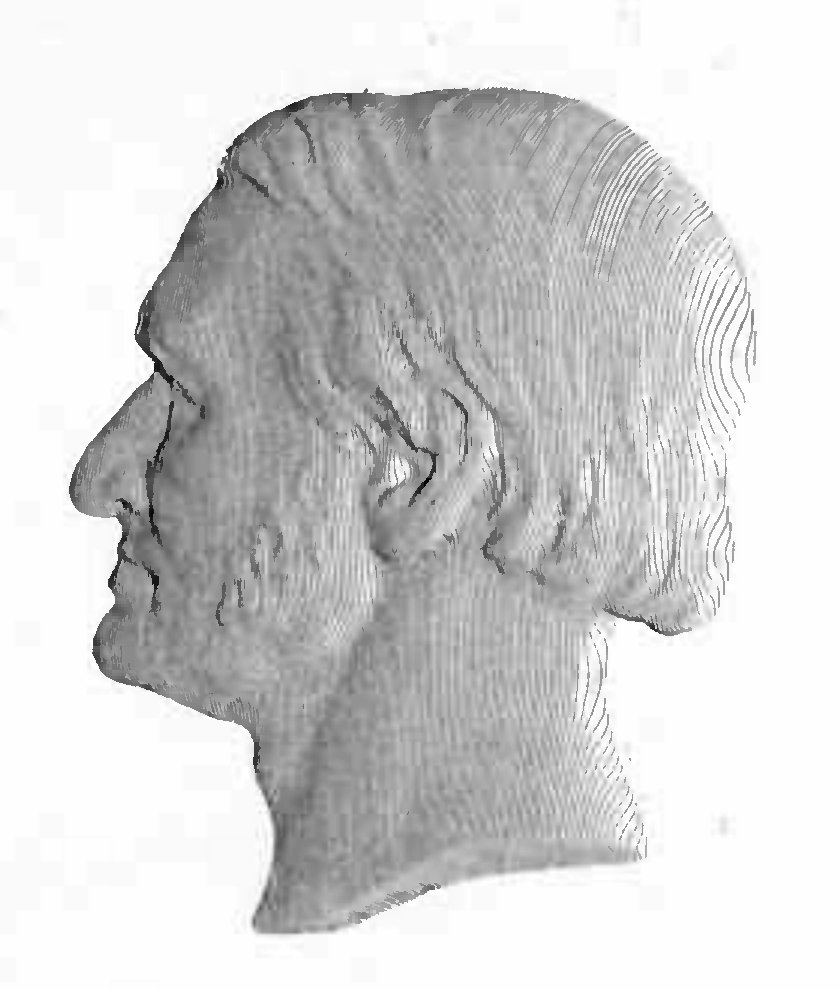
\includegraphics[width=1.6in]{assets/title_profile_contrast.png}\par
\vspace{.3in}{\large SECOND PRINTING\par}
\vspace{.2in}PUBLISHED\par
\smallskip{\small BY THE\par}
\medskip{\small ROYAL SOCIETY OF SCIENCES\par}
\smallskip{\small AT\par}
\medskip{\large GÖTTINGEN\par}
\smallskip1876.
\end{center}
\clearpage
\thispagestyle{empty}\SourceLeaf{11}
\pdfbookmark[0]{A new proof of an arithmetical theorem}{paper-one-title}
\begin{center}
\vspace*{.8in}
{\Large A NEW PROOF\par}
\bigskip{\large OF AN ARITHMETICAL THEOREM\par}
\vspace{.6in}BY\par
\bigskip{\large CARL FRIEDRICH GAUSS\par}
\vspace{.3in}{\small PRESENTED TO THE ROYAL SOCIETY OF SCIENCES JANUARY 15, 1808.\par}
\vspace{.65in}\rule{.85\linewidth}{.3pt}\par
\smallskip{\small Commentationes societatis regiae scientiarum Gottingensis. Vol. \textsc{xvi}.\par}
{\small Gottingae \textsc{mdcccviii}.\par}
\smallskip\rule{.85\linewidth}{.3pt}
\end{center}
\clearpage

\mainmatter
\SourceLeaf{13}
\begin{center}\Large A NEW PROOF\end{center}

\begin{center}\large OF AN ARITHMETICAL THEOREM.\end{center}

\BookRule{35mm}

\Article{1}

Questions in higher arithmetic very often present a singular phenomenon, which occurs much more rarely in analysis and contributes greatly to their charm. In analytic investigations we usually cannot reach new truths unless we have first thoroughly mastered the principles on which they rest and which must, as it were, open the way to them. In arithmetic, by contrast, most elegant new truths very frequently spring forth through induction and a kind of unexpected good fortune; their proofs lie so deeply hidden and are wrapped in such darkness that they elude every attempt and deny access to the keenest investigations. Moreover, so great and so wonderful is the connection among arithmetical truths that at first sight seem utterly different, that quite often, while we are seeking something quite different, we at last most happily reach the proof so greatly desired and previously sought in vain through long reflection, by a path far different from the one expected. Usually, however, truths of this kind are of such a nature that they can be approached by several very different paths, and the paths that first present themselves are not always the shortest. It must therefore certainly be highly valued if, after such a truth has long been investigated in vain, and has then indeed been proved, but by rather obscure detours, we finally succeed in discovering the simplest and genuine path.

\Article{2}

Among the questions discussed in the preceding article, a distinguished place is held by the theorem containing almost the whole theory of quadratic residues, which in the \emph{Arithmetical Investigations} (Section IV) is distinguished by the name of the \emph{fundamental theorem}\SourceLeaf{14}. The illustrious \textsc{Legendre} must undoubtedly be regarded as the \emph{first} discoverer of this most elegant theorem, after the great geometers \textsc{Euler} and \textsc{Lagrange} had, long before, already discovered several of its special cases by induction. I do not pause here to enumerate these men's attempts at a proof; those who wish may consult the work just mentioned. Let me add only, in confirmation of what was said in the preceding article, what concerns my own attempts. I came upon the theorem itself independently in the year 1795, when I was entirely ignorant of everything that had already been worked out in higher arithmetic and wholly cut off from access to the literature. But for an entire year it tormented me and eluded my most strenuous efforts, until at last I obtained the proof given in the fourth section of that work. Afterwards three others, resting on wholly different principles, presented themselves to me; I gave one in the fifth section, and the others, not inferior to it in elegance, I shall make public on another occasion. But all these proofs, although they seem to leave nothing to be desired in rigour, are derived from principles that are too different in kind, perhaps excepting the first, which nevertheless proceeds by more laborious reasoning and is burdened by rather lengthy operations. I therefore do not hesitate to declare that a \emph{genuine} proof has so far been lacking. Let the experts now judge whether the one that I recently succeeded in discovering, and that the following pages present, deserves to be honoured with this name.

\Article{3}

\textsc{Theorem.} \emph{Let $p$ be a positive prime number; $k$ any integer not divisible by $p$;} \emph{use the following definitions:}

\[
\begin{aligned}
A &\quad \text{\emph{collection of the numbers}}\quad 1,\ 2,\ 3\ \dotsfour\ \tfrac12(p-1)\\
B &\quad \text{\emph{collection of these}}\quad \tfrac12(p+1),\ \tfrac12(p+3),\ \tfrac12(p+5)\ \dotsfour\ p-1
\end{aligned}
\]

\emph{Take the products of $k$ by the individual numbers in $A$, and their least positive residues modulo $p$, which are evidently all distinct and belong partly to $A$, partly to} \emph{$B$. Now if altogether $B$ contains $\mu$ of the residues, $k$ will be either a quadratic residue or a quadratic nonresidue of $p$, according as $\mu$ is even or odd.}

\emph{Proof.} Let the residues belonging to $A$ be $a,\ a'\ a''\ \dotsfour$, and the remaining ones, belonging to $B$, be $b,b',b''\dotsfour$. It is clear that the complements of the latter, $p-b,p-b',p-b''\dotsfour$, are all distinct from the numbers $a,\ a',\ a''\ \dotsfour$, but together with these fill out the collection\SourceLeaf{15} $A$. Thus we have

\[
\begin{aligned}
1\pdot2\pdot3\ \dotsfour\ \tfrac12(p-1)=aa' a''\ \dotsfour\ (p-b)(p-b')(p-b'')\ \dotsfour
\end{aligned}
\]

But the latter product evidently becomes

\[
\begin{aligned}
&\equiv(-1)^\mu aa' a''\ \dotsfour\ bb' b''\ \dotsfour\ \equiv(-1)^\mu k\pdot2k\pdot3k\ \dotsfour\ \tfrac12(p-1)k\\
&\equiv(-1)^\mu k^{\frac12(p-1)}\,1\pdot2\pdot3\ \dotsfour\ \tfrac12(p-1) (\mathrm{mod.}p)
\end{aligned}
\]

Hence we have

\[
\begin{aligned}
1\equiv(-1)^\mu k^{\frac12(p-1)}
\end{aligned}
\]

or $k^{\frac12(p-1)}\equiv\pm1$, according as $\mu$ is even or odd; our theorem follows immediately.

\Article{4}

We can greatly shorten the following reasoning by introducing some suitable notation. Thus the symbol $(k,p)$ will denote for us the number of products among

\[
\begin{aligned}
k,\ 2k,\ 3k\ \dotsfour\ \tfrac12(p-1)k,
\end{aligned}
\]

whose least positive residues modulo $p$ exceed half of it. Further, when $x$ is any noninteger quantity, we shall use the symbol $[x]$ to denote the integer immediately smaller than $x$ itself, so that $x-[x]$ is always a positive quantity lying between the limits $0$ and $1$. The following relations are now obtained with little trouble:

I. $[x]+[-x]=-1.$

II. $[x]+h=[x+h]$, whenever $h$ is an integer.

III. $[x]+[h-x]=h-1.$

IV. If $x-[x]$ is a fraction smaller than $\tfrac12$, then $[2x]-2[x]=0$; but if $x-[x]$ is greater than $\tfrac12$, then $[2x]-2[x]=1.$

V. Thus, when the least positive residue of the integer $h$ modulo $p$ lies below $\tfrac12p$, we have $\gbr{\frac{2h}{p}}-2\gbr{\frac{h}{p}}=0$; but when that residue lies above $\tfrac12p$, we have $\gbr{\frac{2h}{p}}-2\gbr{\frac{h}{p}}=1.$

\SourceLeaf{16}
VI. It follows at once that $(k,p)=$

\[
\begin{aligned}
&\gbr{\frac{2k}{p}}+\gbr{\frac{4k}{p}}+\gbr{\frac{6k}{p}}\dotsfour+\gbr{\frac{(p-1)k}{p}}\\
&-2\gbr{\frac{k}{p}}-2\gbr{\frac{2k}{p}}-2\gbr{\frac{3k}{p}}\dotsfour-2\gbr{\frac{\frac12(p-1)k}{p}}.
\end{aligned}
\]

VII. From VI and I we obtain without difficulty

\[
\begin{aligned}
(k,p)+(-k,p)=\tfrac12(p-1)
\end{aligned}
\]

It follows that $-k$ has either the same or the opposite relation to $p$ (insofar as it is a quadratic residue or nonresidue of it) as $+k$, according as $p$ is of the form $4n+1$ or of the form $4n+3$. In the former case $-1$ is evidently a residue, in the latter a nonresidue, of $p$.

\Needspace{10\baselineskip}VIII. We shall transform the formula given in VI as follows. By III we have

\[
\begin{aligned}
\gbr{\frac{(p-1)k}{p}}&=k-1-\gbr{\frac{k}{p}},\\
\gbr{\frac{(p-3)k}{p}}&=k-1-\gbr{\frac{3k}{p}},\\
\gbr{\frac{(p-5)k}{p}}&=k-1-\gbr{\frac{5k}{p}}\dotsfour
\end{aligned}
\]

Applying these substitutions to the last $\frac{p\mp1}{4}$ terms of the upper series in that expression, we have

\Needspace{8\baselineskip}\emph{first}, whenever $p$ is of the form $4n+1$

\[
\begin{aligned}
(k,p)&=\tfrac14(k-1)(p-1)\\
& -2\left\{\gbr{\frac{k}{p}}+\gbr{\frac{3k}{p}}+\gbr{\frac{5k}{p}}\dotsfour+\gbr{\frac{\frac12(p-3)k}{p}}\right\}\\
&\qquad-\left\{\gbr{\frac{k}{p}}+\gbr{\frac{2k}{p}}+\gbr{\frac{3k}{p}}\dotsfour+\gbr{\frac{\frac12(p-1)k}{p}}\right\}
\end{aligned}
\]

\Needspace{8\baselineskip}\emph{second}, whenever $p$ is of the form $4n+3$

\[
\begin{aligned}
(k,p)&=\tfrac14(k-1)(p+1)\\
& -2\left\{\gbr{\frac{k}{p}}+\gbr{\frac{3k}{p}}+\gbr{\frac{5k}{p}}\dotsfour+\gbr{\frac{\frac12(p-1)k}{p}}\right\}\\
&\qquad-\left\{\gbr{\frac{k}{p}}+\gbr{\frac{2k}{p}}+\gbr{\frac{3k}{p}}\dotsfour+\gbr{\frac{\frac12(p-1)k}{p}}\right\}
\end{aligned}
\]

IX. For the special case $k=+2$, the formulas just given yield $(2,p)=\tfrac14(p\mp1)$, taking the upper or lower sign according as $p$ is of the form $4n+1$ or $4n+3$. Thus $(2,p)$ is even, and hence $2Rp$, whenever $p$ is of the form $8n+1$ or $8n+7$; on the other hand, $(2,p)$ is odd and $2Np$, whenever $p$ is of the form $8n+3$ or $8n+5$.

\SourceLeaf{17}
\Needspace{14\baselineskip}\Article{5}

\textsc{Theorem.} \emph{Let $x$ be a positive noninteger quantity, among whose multiples $x$, $2x$,} \emph{$3x\dotsfour$ up to $nx$ none is an integer; put $[nx]=h$, from which it is easily concluded} \emph{that among the multiples of the reciprocal quantity $\frac1x$, $\frac2x$, $\frac3x\dotsfive$ up to $\frac hx$ an integer is likewise not} \emph{found. Then I say that we have}

\[
\begin{aligned}
\left.\begin{aligned}
&[x]+[2x]+[3x]\dotstwo+[nx]\\
&+\gbr{\frac1x}+\gbr{\frac2x}+\gbr{\frac3x}\dotsfour+\gbr{\frac hx}
\end{aligned}\right\}=nh.
\end{aligned}
\]

\emph{Proof.} In the series $[x]+[2x]+[3x]\dotsfour+[nx]$, which we shall put $=\Omega$, the first terms up to and including the term in position $\gbr{\frac1x}$ are evidently all $=0$; the following ones up to the term in position $\gbr{\frac2x}$ are all $=1$; the following ones up to the term in position $\gbr{\frac3x}$ are all $=2$, and so on. Hence we have

\[
\begin{aligned}
\left.\begin{aligned}
\Omega={}&0\times\gbr{\frac1x}\\
&+1\times\left\{\gbr{\frac2x}-\gbr{\frac1x}\right\}\\
&+2\times\left\{\gbr{\frac3x}-\gbr{\frac2x}\right\}\\
&+3\times\left\{\gbr{\frac4x}-\gbr{\frac3x}\right\}\\
&\hspace{12mm}\text{etc.}\\
&+(h-1)\left\{\gbr{\frac hx}-\gbr{\frac{h-1}{x}}\right\}\\
&+h\left\{n-\gbr{\frac hx}\right\}
\end{aligned}\right\}=hn-\gbr{\frac1x}-\gbr{\frac2x}-\gbr{\frac3x}\dotsfour-\gbr{\frac hx}
\end{aligned}
\]

Q. E. D.

\Needspace{12\baselineskip}\Article{6}

\textsc{Theorem.} \emph{If $k,p$ denote any positive odd numbers relatively prime to each other, we have}

\[
\begin{aligned}
\left.\begin{aligned}
&\gbr{\frac kp}+\gbr{\frac{2k}{p}}+\gbr{\frac{3k}{p}}\dotsfour+\gbr{\frac{\frac12(p-1)k}{p}}\\
&+\gbr{\frac pk}+\gbr{\frac{2p}{k}}+\gbr{\frac{3p}{k}}\dotsfour+\gbr{\frac{\frac12(k-1)p}{k}}
\end{aligned}\right\}=\tfrac14(k-1)(p-1).
\end{aligned}
\]

\emph{Proof.} Supposing, as we may, that $k<p$, we have $\frac{\frac12(p-1)k}{p}$ less than $\frac12 k$, but greater than $\frac12(k-1)$, and therefore $\gbr{\frac{\frac12(p-1)k}{p}}=\frac12(k-1)$. Thus the present theorem evidently follows immediately from the preceding one by putting there $\frac kp=x$, $\frac12(p-1)=n$, and hence $\frac12(k-1)=h$.

\SourceLeaf{18}
\Needspace{8\baselineskip}Moreover, it can be proved in a similar manner that, if $k$ is an \emph{even} number relatively prime to $p$, we have

\[
\begin{aligned}
\left.\begin{aligned}
&\gbr{\frac kp}+\gbr{\frac{2k}{p}}+\gbr{\frac{3k}{p}}\dotsfour+\gbr{\frac{\frac12(p-1)k}{p}}\\
&+\gbr{\frac pk}+\gbr{\frac{2p}{k}}+\gbr{\frac{3p}{k}}\dotsfour+\gbr{\frac{\frac12 kp}{k}}
\end{aligned}\right\}=\tfrac14 k(p-1)
\end{aligned}
\]

But we do not dwell on this proposition, which is not needed for our purpose.

\clearpage\Article{7}

The fundamental theorem now follows immediately by combining the preceding theorem with proposition VIII of Article 4. Namely, if $k,p$ denote any unequal positive prime numbers, and we put

\[
\begin{aligned}
(k,p)+\gbr{\frac kp}+\gbr{\frac{2k}{p}}+\gbr{\frac{3k}{p}}\dotsfour+\gbr{\frac{\frac12(p-1)k}{p}}&=L\\
(p,k)+\gbr{\frac pk}+\gbr{\frac{2p}{k}}+\gbr{\frac{3p}{k}}\dotsfour+\gbr{\frac{\frac12(k-1)p}{k}}&=M
\end{aligned}
\]

it is clear from VIII of Article 4 that $L$ and $M$ are always even numbers. But by the theorem of Article 6 we have

\[
\begin{aligned}
L+M=(k,p)+(p,k)+\tfrac14(k-1)(p-1)
\end{aligned}
\]

Thus whenever $\frac14(k-1)(p-1)$ is even, which happens if either both $k,p$ or at least one of them is of the form $4n+1$, $(k,p)$ and $(p,k)$ must necessarily be either both even or both odd. But whenever $\frac14(k-1)(p-1)$ is odd, which happens if both $k,p$ are of the form $4n+3$, one of the numbers $(k,p)$, $(p,k)$ must necessarily be even and the other odd. Thus in the former case the relation of $k$ to $p$ and the relation of $p$ to $k$ (insofar as one is a residue or nonresidue of the other) are identical, and in the latter case opposite.

Q. E. D.

\BookRule{35mm}


\clearpage
\def\BookRunningTitle{Summation of Certain Special Series}
\renewcommand{\Article}[1]{\par\medskip\Needspace{4\baselineskip}\pdfbookmark[1]{Art. #1}{paper-two-art-#1}\centerline{\textbf{#1.}}\nobreak\smallskip}
\clearpage\thispagestyle{empty}\SourceLeaf{19}
\pdfbookmark[0]{Summation of certain special series}{paper-two-title}
\begin{center}
\vspace*{.6in}{\large SUMMATION\par}
\bigskip{\Large OF CERTAIN\par}
\bigskip{\large SPECIAL SERIES\par}
\vspace{.65in}BY\par
\bigskip{\large CARL FRIEDRICH GAUSS\par}
\vspace{.3in}{\small PRESENTED TO THE SOCIETY AUGUST XXIV, MDCCCVIII.\par}
\vspace{.6in}\rule{.85\linewidth}{.3pt}\par
\smallskip{\small Commentationes societatis regiae scientiarum Gottingensis recentiores. Vol. \textsc{i}.\par}
{\small Gottingae \textsc{mdcccxi}.\par}
\smallskip\rule{.85\linewidth}{.3pt}
\end{center}

\clearpage
\SourceLeaf{21}
\begin{center}\Large SUMMATION\end{center}

\begin{center}\large OF CERTAIN SPECIAL SERIES.\end{center}

\BookRule{22mm}

\Article{1}

Among the more notable truths to which the theory of circle division has opened the way, the summation proposed in Disquiss. Arithmet., Article 356, holds a distinguished place. This is due both to its particular elegance and remarkable fruitfulness, which another investigation will later give us occasion to discuss more fully, and to the unusual difficulties that beset its rigorous and complete proof.\quad These difficulties should have been all the less expected because they concern a certain restriction of the theorem more than the theorem itself: once this restriction is disregarded, a proof is immediately available and follows very easily from the theory developed in that work.\quad The theorem was given there in the following form.\quad Suppose that $n$ is a prime number. Represent all the quadratic residues of $n$ between $1$ and $n-1$ inclusive by $a$, and all the nonresidues between the same limits by $b$; finally, let $\omega$ be the arc $\frac{360^{0}}{n}$, and $k$ any fixed integer not divisible by $n$. Then we have

I.\quad for a value of $n$ of the form $4m+1$,

\[
\begin{aligned}
\Sigma\cos ak\omega&=-\tfrac12\pm\tfrac12\surd n\\
\Sigma\cos bk\omega&=-\tfrac12\mp\tfrac12\surd n,\ \text{and hence}\\
\Sigma\cos ak\omega-\Sigma\cos bk\omega&=\pm\surd n\\
\Sigma\sin ak\omega&=0\\
\Sigma\sin bk\omega&=0
\end{aligned}
\]

\SourceLeaf{22}
II.\quad for a value of $n$ of the form $4m+3$,

\[
\begin{aligned}
\Sigma\cos ak\omega&=-\tfrac12\\
\Sigma\cos bk\omega&=-\tfrac12\\
\Sigma\sin ak\omega&=\pm\tfrac12\surd n\\
\Sigma\sin bk\omega&=\mp\tfrac12\surd n\\
\Sigma\sin ak\omega-\Sigma\sin bk\omega&=\pm\surd n
\end{aligned}
\]

These summations were proved with full rigor in the place cited, and the only difficulty that remains here is to determine the \emph{sign} to be placed before the radical.\quad It can indeed be shown without difficulty that this sign depends on the number $k$ to the following extent: the \emph{same} sign must hold for all values of $k$ that are quadratic residues of $n$, and the opposite sign for all values of $k$ that are quadratic nonresidues of $n$.\quad Thus the whole question turns on the value $k=1$: as soon as the sign for this value is known, the signs for all the other values of $k$ are immediately available as well.\quad Yet this very question, which at first seems to be among the easier ones, presents us with unforeseen difficulties, and the method that had guided us this far without impediment utterly refuses any further help.

\Article{2}

Before proceeding further, it will be useful to work out some examples of our summation numerically; we should, however, first make a few general observations.

I.\quad In the case where $n$ is a prime number of the form $4m+1$, let all the quadratic residues of $n$ between $1$ and $\frac12(n-1)$ inclusive be represented by $a'$, and all the nonresidues between the same limits by $b'$. All the $n-a'$ are known to be among the $a$, and all the $n-b'$ among the $b$. Since all the $a'$, $b'$, $n-a'$, $n-b'$ together evidently make up the entire collection of numbers $1$, $2$, $3\dotsfour$ $n-1$, all the $a'$ together with all the $n-a'$ comprise all the $a$; likewise all the $b'$ together with all the $n-b'$ comprise all the $b$.\quad Hence

\SourceLeaf{23}
\[
\begin{aligned}
\Sigma\cos ak\omega&=\Sigma\cos a'k\omega+\Sigma\cos(n-a')k\omega\\
\Sigma\cos bk\omega&=\Sigma\cos b'k\omega+\Sigma\cos(n-b')k\omega\\
\Sigma\sin ak\omega&=\Sigma\sin a'k\omega+\Sigma\sin(n-a')k\omega\\
\Sigma\sin bk\omega&=\Sigma\sin b'k\omega+\Sigma\sin(n-b')k\omega
\end{aligned}
\]

Now, since $\cos(n-a')k\omega=\cos a'k\omega$, $\cos(n-b')k\omega=\cos b'k\omega$, $\sin(n-a')k\omega=-\sin a'k\omega$, $\sin(n-b')k\omega=-\sin b'k\omega$, it follows at once that

\[
\begin{aligned}
\Sigma\sin ak\omega&=\Sigma\sin a'k\omega-\Sigma\sin a'k\omega=0\\
\Sigma\sin bk\omega&=\Sigma\sin b'k\omega-\Sigma\sin b'k\omega=0
\end{aligned}
\]

The summation of the cosines takes the form

\[
\begin{aligned}
\Sigma\cos ak\omega&=2\Sigma\cos a'k\omega\\
\Sigma\cos bk\omega&=2\Sigma\cos b'k\omega
\end{aligned}
\]

so that we must have

\[
\begin{aligned}
1+4\Sigma\cos a'k\omega&=\pm\surd n\\
1+4\Sigma\cos b'k\omega&=\mp\surd n\\
2\Sigma\cos a'k\omega-2\Sigma\cos b'k\omega&=\pm\surd n
\end{aligned}
\]

\Needspace{9\baselineskip}II.\quad In the case where $n$ is of the form $4m+3$, the complement of any residue $a$ to $n$ is a nonresidue, and the complement of any $b$ is a residue. Thus all the $n-a$ coincide with all the $b$, and all the $n-b$ with all the $a$. This gives

\[
\begin{aligned}
\Sigma\cos ak\omega=\Sigma\cos(n-b)k\omega=\Sigma\cos bk\omega
\end{aligned}
\]

Since all the $a$ and $b$ together make up all the numbers $1$, $2$, $3\dotsfour n-1$, and hence $\Sigma\cos ak\omega+\Sigma\cos bk\omega=\cos k\omega+\cos2k\omega+\cos3k\omega+\text{etc.}$ $+\cos(n-1)k\omega=-1$, the summations

\[
\begin{aligned}
\Sigma\cos ak\omega&=-\tfrac12\\
\Sigma\cos bk\omega&=-\tfrac12
\end{aligned}
\]

follow immediately.\quad Likewise,

\[
\begin{aligned}
\Sigma\sin ak\omega=\Sigma\sin(n-b)k\omega=-\Sigma\sin bk\omega
\end{aligned}
\]

\SourceLeaf{24}
which shows how the two summations

\[
\begin{aligned}
2\Sigma\sin ak\omega&=\pm\surd n\\
2\Sigma\sin bk\omega&=\mp\surd n
\end{aligned}
\]

depend on one another.

\Article{3}

Here are the numerical calculations for several examples:

I.\quad For $n=5$ there is one value of $a'$, namely $a'=1$, and one value of $b'$, namely $b'=2$. We have

\[
\begin{aligned}
\cos\omega=+0{,}3090169944\qquad\cos2\omega=-0{,}8090169944
\end{aligned}
\]

and hence $1+4\cos\omega=+\surd5$,\quad $1+4\cos2\omega=-\surd5$.

II.\quad For $n=13$ there are three values of $a'$, namely $1$, $3$, $4$, and as many values of $b'$, namely $2$, $5$, $6$. We calculate

{\small\setlength{\arraycolsep}{2.5pt}\renewcommand{\arraystretch}{1.15}
\[
\begin{array}{rclcrcl}
\cos\omega&=&+0{,}8854560257&\qquad&\cos2\omega&=&+0{,}5680647467\\
\cos3\omega&=&+0{,}1205366803&\qquad&\cos5\omega&=&-0{,}7485107482\\
\cos4\omega&=&-0{,}3546048870&\qquad&\cos6\omega&=&-0{,}9709418174\\\cline{1-3}\cline{5-7}
\text{Sum}&=&+0{,}6513878190&\qquad&\text{Sum}&=&-1{,}1513878189
\end{array}
\]
}

Hence $1+4\Sigma\cos a'\omega=+\surd13$,\quad $1+4\Sigma\cos b'\omega=-\surd13$.

\Needspace{13\baselineskip}III.\quad For $n=17$ we have four values of $a'$, namely $1$, $2$, $4$, $8$, and as many values of $b'$, namely $3$, $5$, $6$, $7$.\quad The cosines are therefore calculated as follows:

{\small\setlength{\arraycolsep}{2.5pt}\renewcommand{\arraystretch}{1.15}
\[
\begin{array}{rclcrcl}
\cos\omega&=&+0{,}9324722294&\qquad&\cos3\omega&=&+0{,}4457383558\\
\cos2\omega&=&+0{,}7390089172&\qquad&\cos5\omega&=&-0{,}2736629901\\
\cos4\omega&=&+0{,}0922683595&\qquad&\cos6\omega&=&-0{,}6026346364\\
\cos8\omega&=&-0{,}9829730997&\qquad&\cos7\omega&=&-0{,}8502171357\\\cline{1-3}\cline{5-7}
\text{Sum}&=&+0{,}7807764064&\qquad&\text{Sum}&=&-1{,}2807764065
\end{array}
\]
}

Hence $1+4\Sigma\cos a'\omega=+\surd17$,\quad $1+4\Sigma\cos b'\omega=-\surd17$.

\SourceLeaf{25}
IV.\quad For $n=3$ there is just one value of $a$, namely $a=1$, to which corresponds

\[
\begin{aligned}
\sin\omega=+0{,}8660254038
\end{aligned}
\]

Hence $2\sin\omega=+\surd3$.

V.\quad For $n=7$ there are three values of $a$, namely $1$, $2$, $4$. These give the sines

{\small\setlength{\arraycolsep}{2.5pt}\renewcommand{\arraystretch}{1.15}
\[
\begin{array}{rcll}
\sin\omega&=&+0{,}7818314825&\\
\sin2\omega&=&+0{,}9749279122&\\
\sin4\omega&=&-0{,}4338837391&\\\cline{1-3}
\text{Sum}&=&+1{,}3228756556,&\text{and hence }2\Sigma\sin a\omega=+\surd7.
\end{array}
\]
}

VI.\quad For $n=11$ the values of $a$ are $1$, $3$, $4$, $5$, $9$, to which correspond the sines

{\small\setlength{\arraycolsep}{2.5pt}\renewcommand{\arraystretch}{1.15}
\[
\begin{array}{rcll}
\sin\omega&=&+0{,}5406408175&\\
\sin3\omega&=&+0{,}9898214419&\\
\sin4\omega&=&+0{,}7557495744&\\
\sin5\omega&=&+0{,}2817325568&\\
\sin9\omega&=&-0{,}9096319954&\\\cline{1-3}
\text{Sum}&=&+1{,}6583123952,&\text{and hence }2\Sigma\sin a\omega=+\surd11.
\end{array}
\]
}

\Needspace{19\baselineskip}VII.\quad For $n=19$ the values of $a$ are $1$, $4$, $5$, $6$, $7$, $9$, $11$, $16$, $17$, to which correspond the sines

{\small\setlength{\arraycolsep}{2.5pt}\renewcommand{\arraystretch}{1.15}
\[
\begin{array}{rcll}
\sin\omega&=&+0{,}3246994692&\\
\sin4\omega&=&+0{,}9694002659&\\
\sin5\omega&=&+0{,}9965844930&\\
\sin6\omega&=&+0{,}9157733267&\\
\sin7\omega&=&+0{,}7357239107&\\
\sin9\omega&=&+0{,}1645945903&\\
\sin11\omega&=&-0{,}4759473930&\\
\sin16\omega&=&-0{,}8371664783&\\
\sin17\omega&=&-0{,}6142127127&\\\cline{1-3}
\text{Sum}&=&+2{,}1794494718,&\text{and hence }2\Sigma\sin a\omega=+\surd19.
\end{array}
\]
}

\SourceLeaf{26}
\Article{4}

In all these examples the radical takes the positive sign. This is also easily confirmed for the larger values $n=23$, $n=29$, etc., and already makes it highly probable that the same holds in general.\quad But a proof of this phenomenon cannot be drawn from the principles set out in the place cited, and it must with full justification be regarded as a matter for deeper investigation.\quad The purpose of this paper is therefore to present a rigorous proof of this most elegant theorem, attempted in vain in various ways over several years and finally achieved through unusual and quite subtle considerations. At the same time we shall bring the theorem to a far greater degree of generality, preserving, or rather increasing, its elegance.\quad Finally, as a crowning addition, we shall show the remarkable and very close connection between this summation and another arithmetical theorem of the greatest importance.\quad We hope that these investigations will themselves be welcome to geometers, and that the methods by which we have accomplished all this, and which may also be useful on other occasions, will be considered worthy of their attention.

\Article{5}

Our proof comes from considering a special kind of series whose terms depend on expressions such as

\[
\begin{aligned}
\frac{(1-x^m)\,(1-x^{m-1})\,(1-x^{m-2})\dotsfour(1-x^{m-\mu+1})}{(1-x)\,(1-xx)\,(1-x^3)\dotsfive(1-x^\mu)}
\end{aligned}
\]

For brevity we shall denote such a fraction by $(m,\mu)$, and first make a few general observations about functions of this kind.

\Needspace{19\baselineskip}I.\quad Whenever $m$ is a positive integer less than $\mu$, the function $(m,\mu)$ evidently vanishes, since the numerator contains the factor $1-x^0$.\quad For $m=\mu$, the factors in the numerator are identical, in reverse order, to those in the denominator, so that $(\mu,\mu)=1$. Finally, for the case where $m$ is a positive integer greater than $\mu$, we have the formulas

\[
\begin{aligned}
(\mu+1,\mu)&=\frac{1-x^{\mu+1}}{1-x}=(\mu+1,1)\\
(\mu+2,\mu)&=\frac{(1-x^{\mu+2})\,(1-x^{\mu+1})}{(1-x)\qquad(1-xx)}=(\mu+2,2)\\
(\mu+3,\mu)&=\frac{(1-x^{\mu+3})(1-x^{\mu+2})(1-x^{\mu+1})}{(1-x)\qquad(1-xx)\qquad(1-x^3)}=(\mu+3,3)\ \text{etc.}
\end{aligned}
\]

\SourceLeaf{27}
or, in general,

\[
\begin{aligned}
(m,\mu)=(m,m-\mu)
\end{aligned}
\]

II.\quad Further, it is easily confirmed that in general

\[
\begin{aligned}
(m,\mu+1)=(m-1,\mu+1)+x^{m-\mu-1}(m-1,\mu)
\end{aligned}
\]

and since we likewise have

\[
\begin{aligned}
(m-1,\mu+1)&=(m-2,\mu+1)+x^{m-\mu-2}(m-2,\mu)\\
(m-2,\mu+1)&=(m-3,\mu+1)+x^{m-\mu-3}(m-3,\mu)\\
(m-3,\mu+1)&=(m-4,\mu+1)+x^{m-\mu-4}(m-4,\mu),\ \text{etc.}
\end{aligned}
\]

and can continue this series as far as

\[
\begin{aligned}
(\mu+2,\mu+1)&=(\mu+1,\mu+1)+x(\mu+1,\mu)\\
&=(\mu,\mu)+x(\mu+1,\mu)
\end{aligned}
\]

provided that $m$ is a positive integer greater than $\mu+1$, we obtain

\[
\begin{aligned}
(m,\mu+1)&=(\mu,\mu)+x(\mu+1,\mu)+xx(\mu+2,\mu)\\
&\qquad+x^3(\mu+3,\mu)+\text{etc.}\\
&\qquad+x^{m-\mu-1}(m-1,\mu)
\end{aligned}
\]

\Needspace{16\baselineskip}This shows that if, for some fixed value of $\mu$, every function $(m,\mu)$ is a polynomial whenever $m$ is a positive integer, then every function $(m,\mu+1)$ must also be a polynomial.\quad Since that supposition holds for $\mu=1$, it therefore also holds for $\mu=2$, and hence for $\mu=3$, etc. That is, in general, for any positive integral value of $m$, $(m,\mu)$ is a polynomial, or equivalently the product

\[
\begin{aligned}
(1-x^m)(1-x^{m-1})(1-x^{m-2})\dotsfour(1-x^{m-\mu+1})
\end{aligned}
\]

is divisible by

\[
\begin{aligned}
(1-x)(1-x^2)(1-x^3)\dotsfour(1-x^\mu)
\end{aligned}
\]

\clearpage\Needspace{14\baselineskip}\Article{6}

We shall now consider two series, both of which can lead to our goal.\quad The first series is

\SourceLeaf{28}
\[
\begin{aligned}
&1-\frac{1-x^m}{1-x}+\frac{(1-x^m)\,(1-x^{m-1})}{(1-x)\,(1-xx)}\\
&\qquad-\frac{(1-x^m)(1-x^{m-1})(1-x^{m-2})}{(1-x)\quad(1-xx)\quad(1-x^3)}+\text{etc.}
\end{aligned}
\]

or

\[
\begin{aligned}
1-(m,1)+(m,2)-(m,3)+(m,4)-\text{etc.}
\end{aligned}
\]

which for brevity we shall denote by $f(x,m)$.\quad First, it is immediately evident that whenever $m$ is a positive integer this series \emph{terminates} after its term in position $m+1$ (with $=\pm1$), and that in this case its sum must therefore be a finite polynomial in $x$.\quad Further, Article 5, II, shows that in general, for any value of $m$,

\[
\begin{aligned}
1&=1\\
-(m,1)&=-(m-1,1)-x^{m-1}\\
+(m,2)&=+(m-1,2)+x^{m-2}(m-1,1)\\
-(m,3)&=-(m-1,3)-x^{m-3}(m-1,2),\ \text{etc.}
\end{aligned}
\]

and hence

\[
\begin{aligned}
f(x,m)&=1-x^{m-1}-(1-x^{m-2})(m-1,1)\\
&\qquad+(1-x^{m-3})(m-1,2)\\
&\qquad-(1-x^{m-4})(m-1,3)+\text{etc.}
\end{aligned}
\]

But evidently

\[
\begin{aligned}
(1-x^{m-2})(m-1,1)&=(1-x^{m-1})(m-2,1)\\
(1-x^{m-3})(m-1,2)&=(1-x^{m-1})(m-2,2)\\
(1-x^{m-4})(m-1,3)&=(1-x^{m-1})(m-2,3),\ \text{etc.}
\end{aligned}
\]

from which we deduce the equation

\[
\begin{aligned}
f(x,m)=(1-x^{m-1})f(x,m-2)\ .\ .\ .\ .\ .\ .\ .\ .\ [1]
\end{aligned}
\]

\clearpage\Needspace{11\baselineskip}\Article{7}

Since for $m=0$ we have $f(x,m)=1$, the formula just found gives

\[
\begin{aligned}
f(x,2)&=1-x\\
f(x,4)&=(1-x)(1-x^3)\\
f(x,6)&=(1-x)(1-x^3)(1-x^5)\\
f(x,8)&=(1-x)(1-x^3)(1-x^5)(1-x^7),\ \text{etc.}
\end{aligned}
\]

or, in general, for any even value of $m$,

\[
\begin{aligned}
f(x,m)=(1-x)(1-x^3)(1-x^5)\dotsfour(1-x^{m-1})\ .\ .\ .\ [2].
\end{aligned}
\]

\SourceLeaf{29}
Conversely, since for $m=1$ we have $f(x,m)=0$, we also have

\[
\begin{aligned}
f(x,3)&=0\\
f(x,5)&=0\\
f(x,7)&=0\ \text{etc.}
\end{aligned}
\]

\Needspace{5\baselineskip}or, in general, for any odd value of $m$,

\[
\begin{aligned}
f(x,m)=0
\end{aligned}
\]

The latter summation could, moreover, already have been derived from the fact that in the series

\[
\begin{aligned}
1-(m,1)+(m,2)-(m,3)+\text{etc.}+(m,m-1)-(m,m)
\end{aligned}
\]

the last term cancels the first, the next to last cancels the second, etc.

\Article{8}

For our purpose the case where $m$ is a positive odd integer is sufficient. But the unusual nature of the matter makes it worthwhile to add a few remarks about the cases where $m$ is fractional or negative.\quad Our series then evidently no longer terminates, but continues to infinity; it is also easily seen that it becomes divergent whenever $x$ is given a value less than $1$, so that its summation must be restricted to values of $x$ greater than $1$.

\Needspace{13\baselineskip}By formula [1] of Article 6 we have

\[
\begin{aligned}
f(x,-2)&=\frac{1}{1-\frac1x}\\[8pt]
f(x,-4)&=\frac{1}{1-\frac1x}\pdot\frac{1}{1-\frac1{x^3}}\\[8pt]
f(x,-6)&=\frac{1}{1-\frac1x}\pdot\frac{1}{1-\frac1{x^3}}\pdot\frac{1}{1-\frac1{x^5}},\ \text{etc.}
\end{aligned}
\]

so that the value of the function $f(x,m)$ can also be given in finite terms for a negative even integral value of $m$.\quad For the remaining values of $m$, however, we shall convert the function $f(x,m)$ into an \emph{infinite product} as follows.

As $m$ tends to a negative \emph{infinite} value, the function $f(x,m)$ becomes

\SourceLeaf{30}
\[
\begin{aligned}
&1+\frac1{x-1}+\frac1{x-1}\pdot\frac1{xx-1}\\
&\qquad+\frac1{x-1}\pdot\frac1{xx-1}\pdot\frac1{x^3-1}+\text{etc.}
\end{aligned}
\]

This series is therefore equal to the infinite product

\[
\begin{aligned}
\frac1{1-\frac1x}\pdot\frac1{1-\frac1{x^3}}\pdot\frac1{1-\frac1{x^5}}\pdot\frac1{1-\frac1{x^7}}\;\text{etc. to infinity.}
\end{aligned}
\]

Further, since in general

\[
\begin{aligned}
f(x,m)&=f(x,m-2\lambda)\pdot(1-x^{m-1})(1-x^{m-3})\\
&\qquad(1-x^{m-5})\dotstwo(1-x^{m-2\lambda+1})
\end{aligned}
\]

we have

\[
\begin{aligned}
f(x,m)&=f(x,-\infty)\pdot(1-x^{m-1})(1-x^{m-3})(1-x^{m-5})\\
&\qquad\text{etc. to infinity.}\\
&=\frac{1-x^{m-1}}{1-x^{-1}}\pdot\frac{1-x^{m-3}}{1-x^{-3}}\pdot\frac{1-x^{m-5}}{1-x^{-5}}\pdot\frac{1-x^{m-7}}{1-x^{-7}}\\
&\qquad\text{etc. to infinity.}
\end{aligned}
\]

whose factors evidently converge ever more closely to unity as they continue.

The case $m=-1$ deserves particular attention. Here

\[
\begin{aligned}
f(x,-1)=1+x^{-1}+x^{-3}+x^{-6}+x^{-10}+\text{etc.}
\end{aligned}
\]

\Needspace{9\baselineskip}This series is therefore equal to the infinite product

\[
\begin{aligned}
\frac{1-x^{-2}}{1-x^{-1}}\pdot\frac{1-x^{-4}}{1-x^{-3}}\pdot\frac{1-x^{-6}}{1-x^{-5}}\;\text{etc.}
\end{aligned}
\]

or, writing $x$ for $x^{-1}$, we obtain

\[
\begin{aligned}
1+x+x^3+x^6+\text{etc.}&=\frac{1-xx}{1-x}\pdot\frac{1-x^4}{1-x^3}\pdot\frac{1-x^6}{1-x^5}\\
&\qquad\pdot\frac{1-x^8}{1-x^7}\;\text{etc.}
\end{aligned}
\]

This equality between two rather intricate expressions, to which we shall return on another occasion, is certainly very remarkable.

\Needspace{15\baselineskip}\Article{9}

Secondly, we shall consider the series

\[
\begin{aligned}
&1+x^{\frac12}\frac{1-x^m}{1-x}+x\frac{(1-x^m)(1-x^{m-1})}{(1-x)(1-xx)}\\
&\qquad+x^{\frac32}\frac{(1-x^m)(1-x^{m-1})(1-x^{m-2})}{(1-x)(1-xx)(1-x^3)}+\text{etc.}
\end{aligned}
\]

or

\[
\begin{aligned}
1+x^{\frac12}(m,1)+x(m,2)+x^{\frac32}(m,3)+xx(m,4)+\text{etc.}
\end{aligned}
\]

which we shall denote by $F(x,m)$.\quad We restrict this investigation to the case where $m$ is a positive integer, so that this series too always ends
\SourceLeaf{31}
at its term in position $m+1$ (with $=x^{\frac12m}(m,m)$).\quad Since

\[
\begin{aligned}
(m,m)=1,\quad(m,m-1)=(m,1),\quad(m,m-2)=(m,2),\;\text{etc.}
\end{aligned}
\]

the series can also be written as follows:

\[
\begin{aligned}
F(x,m)&=x^{\frac12m}+x^{\frac12(m-1)}(m,1)\\&\qquad+x^{\frac12(m-2)}(m,2)+x^{\frac12(m-3)}(m,3)+\text{etc.}
\end{aligned}
\]

This gives

\[
\begin{aligned}
(1+x^{\frac12m+\frac12})F(x,m)&=1+x^{\frac12}(m,1)+x(m,2)\\&\qquad+x^{\frac32}(m,3)+\text{etc.}\\
&+x^{\frac12}\pdot x^m+x\pdot x^{m-1}(m,1)\\&\qquad+x^{\frac32}\pdot x^{m-2}(m,2)+\text{etc.}
\end{aligned}
\]

Since we have (Article 5, II)

\[
\begin{aligned}
(m,1)+x^m&=(m+1,1)\\
(m,2)+x^{m-1}(m,1)&=(m+1,2)\\
(m,3)+x^{m-2}(m,2)&=(m+1,3),\;\text{etc.}
\end{aligned}
\]

we obtain

\[
\begin{aligned}
(1+x^{\frac12m+\frac12})F(x,m)=F(x,m+1)\ .\; .\; .\; .\; .\; .\; .\ [3]
\end{aligned}
\]

But $F(x,0)=1$, so that

\[
\begin{aligned}
F(x,1)&=1+x^{\frac12}\\
F(x,2)&=(1+x^{\frac12})(1+x)\\
F(x,3)&=(1+x^{\frac12})(1+x)(1+x^{\frac32}),\;\text{etc.}
\end{aligned}
\]

or, in general,

\[
\begin{aligned}
F(x,m)&=(1+x^{\frac12})(1+x)(1+x^{\frac32})\\&\qquad\dotsfour(1+x^{\frac12m})\ .\; .\; .\; .\quad[4]
\end{aligned}
\]

\Needspace{12\baselineskip}\Article{10}

With these preliminary investigations in place, let us now come closer to our aim.\quad For a prime value of $n$, the squares $1$, $4$, $9\dotsfour(\frac12(n-1))^2$ are all incongruent to one another modulo $n$; their least residues for this modulus must therefore be identical to the numbers $a$, and hence

\[
\begin{aligned}
\Sigma\cos ak\omega&=\cos k\omega+\cos4k\omega+\cos9k\omega\\&\qquad+\text{etc.}+\cos(\tfrac12(n-1))^2k\omega\\
\Sigma\sin ak\omega&=\sin k\omega+\sin4k\omega+\sin9k\omega\\&\qquad+\text{etc.}+\sin(\tfrac12(n-1))^2k\omega
\end{aligned}
\]

Likewise, since the same squares $1$, $4$, $9\dotsfour(\frac12(n-1))^2$, in reverse order, are congruent to $(\frac12(n+1))^2$, $(\frac12(n+3))^2$, $(\frac12(n+5))^2\dotsfive(n-1)^2$, we also have

\SourceLeaf{32}

\[
\begin{aligned}
\Sigma\cos ak\omega&=\cos(\tfrac12(n+1))^2k\omega\\&\qquad+\cos(\tfrac12(n+3))^2k\omega+\text{etc.}+\cos(n-1)^2k\omega\\
\Sigma\sin ak\omega&=\sin(\tfrac12(n+1))^2k\omega\\&\qquad+\sin(\tfrac12(n+3))^2k\omega+\text{etc.}+\sin(n-1)^2k\omega
\end{aligned}
\]

\Needspace{9\baselineskip}Thus, putting

\[
\begin{aligned}
T&=1+\cos k\omega+\cos4k\omega+\cos9k\omega\\&\qquad+\text{etc.}+\cos(n-1)^2k\omega\\
U&=\phantom{1+}\sin k\omega+\sin4k\omega+\sin9k\omega\\&\qquad+\text{etc.}+\sin(n-1)^2k\omega
\end{aligned}
\]

we obtain

\[
\begin{aligned}
1+2\Sigma\cos ak\omega&=T\\
2\Sigma\sin ak\omega&=U
\end{aligned}
\]

This shows that the summations proposed in Article 1 depend on summing the series $T$ and $U$. We shall therefore leave the former aside and direct our investigation to these, carrying it out generally enough to include both prime values of $n$ and any composite values.\quad We shall, however, suppose that the number $k$ is relatively prime to $n$: the case where $k$ and $n$ have a common divisor can be reduced to this one without difficulty.

\Needspace{12\baselineskip}\Article{11}

Let us denote the imaginary quantity $\surd{-1}$ by $i$ and put

\[
\begin{aligned}
\cos k\omega+i\sin k\omega=r
\end{aligned}
\]

Then $r^n=1$, or $r$ is a root of the equation $r^n-1=0$.\quad It is easy to see that all the numbers $k$, $2k$, $3k\dotsfour(n-1)k$ are not divisible by $n$ and are incongruent to one another modulo $n$. Thus the powers of $r$

\[
\begin{aligned}
1,\;r,\;rr,\;r^3\dotsfour r^{n-1}
\end{aligned}
\]

are all unequal, while each also satisfies the equation $x^n-1=0$. For this reason these powers represent \emph{all} the roots of the equation $x^n-1=0$.

These conclusions would not hold if $k$ had a common divisor with $n$. For if $\nu$ were such a common divisor, $k\pdot\dfrac n\nu$ would be divisible by $n$, and hence a power lower than $r^n$, namely $r^{\frac n\nu}$, would equal unity.\quad In this case, therefore, the powers of $r$ represent at most $\dfrac n\nu$ roots of the equation $x^n-1=0$, and indeed give that many distinct roots if $\nu$ is the \emph{greatest} common divisor of the numbers\SourceLeaf{33}
$k$, $n$.\quad In our case, where $k$ and $n$ are supposed relatively prime, $r$ can conveniently be called a \emph{proper root} of the equation $x^n-1=0$. In the other case, where $k$ and $n$ have a (greatest) common divisor $\nu$, $r$ would be called an \emph{improper root} of that equation. Then, however, the same $r$ would evidently be a proper root of the equation $x^{\frac n\nu}-1=0$.\quad The simplest improper root is unity, and when $n$ is a prime number there are no other improper roots at all.

\Needspace{13\baselineskip}\Article{12}

Now, if we put

\[
\begin{aligned}
W=1+r+r^4+r^9+\text{etc.}+\text{etc.}+r^{(n-1)^2}
\end{aligned}
\]

we evidently have $W=T+iU$, so that $T$ is the real part of $W$, and $U$ is obtained from the imaginary part of $W$ by removing the factor $i$.\quad The whole question is therefore reduced to finding the sum $W$. For this purpose we can use either the series considered in Article 6 or the one we showed how to sum in Article 9; the former, however, is less suitable when $n$ is even.\quad Nevertheless, we hope that readers will welcome our treating the case where $n$ is odd by two methods.

First, then, suppose that $n$ is an odd number, that $r$ denotes any proper root of the equation $x^n-1=0$, and that in the function $f(x,m)$ we put $x=r$ and $m=n-1$.\quad We evidently obtain

\[
\begin{aligned}
\frac{1-x^m}{1-x}&=\frac{1-r^{-1}}{1-r}=-r^{-1}\\
\frac{1-x^{m-1}}{1-xx}&=\frac{1-r^{-2}}{1-rr}=-r^{-2}\\
\frac{1-x^{m-2}}{1-x^3}&=\frac{1-r^{-3}}{1-r^3}=-r^{-3},\;\text{etc.}
\end{aligned}
\]

as far as

\[
\begin{aligned}
\frac{1-x}{1-x^m}=\frac{1-r^{-m}}{1-r^m}=-r^{-m}
\end{aligned}
\]

(It is worth pointing out that these equations hold only insofar as $r$ is supposed to be a proper root: if $r$ were an improper root, the numerator and denominator of some of these fractions would vanish together, and the fractions would therefore become indeterminate).

From this we deduce the following equation

\SourceLeaf{34}

\[
\begin{aligned}
f(r,n-1)&=1+r^{-1}+r^{-3}+r^{-6}+\text{etc.}+r^{-\frac12(n-1)n}\\
&=(1-r)(1-r^3)(1-r^5)\dotsfive(1-r^{n-2})
\end{aligned}
\]

The same equation still holds if we replace $r$ by $r^\lambda$, where $\lambda$ denotes any integer relatively prime to $n$: for then $r^\lambda$ too is a proper root of the equation $x^n-1=0$.\quad Let us therefore replace $r$ by $r^{n-2}$, or equivalently $r^{-2}$. We obtain

\[
\begin{aligned}
&1+r^2+r^6+r^{12}+\text{etc.}+r^{(n-1)n}\\&\qquad=(1-r^{-2})(1-r^{-6})(1-r^{-10})\ldots(1-r^{-2(n-2)})
\end{aligned}
\]

Let us multiply both sides of this equation by

\[
\begin{aligned}
r\pdot r^3\pdot r^5\dotsfour r^{(n-2)}=r^{\frac14(n-1)^2}
\end{aligned}
\]

\Needspace{13\baselineskip}and, since

\[
\begin{aligned}
r^{2+\frac14(n-1)^2}&=r^{\frac14(n-3)^2},\\r^{(n-1)n+\frac14\,n-1)^2}=r^{\frac14(n+1)^2}\\
r^{6+\frac14(n-1)^2}&=r^{\frac14(n-5)^2},\\r^{(n-2)(n-1)+\frac14(n-1)^2}=r^{\frac14(n+3)^2}\\
r^{12+\frac14(n-1)^2}&=r^{\frac14(n-7)^2},\\r^{(n-3)(n-2)+\frac14(n-1)^2}=r^{\frac14(n+5)^2},\;\text{etc.}
\end{aligned}
\]

the following equation results:

\[
\begin{aligned}
&r^{\frac14(n-1)^2}+r^{\frac14(n-3)^2}+r^{\frac14(n-5)^2}+\text{etc.}+r+1\\
&+r^{\frac14(n+1)^2}+r^{\frac14(n+3)^2}+r^{\frac14(n+5)^2}\\&\qquad+\text{etc.}+r^{\frac14(2n-2)^2}\\
&\qquad=(r-r^{-1})(r^3-r^{-3})(r^5-r^{-5})\dotsfour(r^{n-2}-r^{-n+2})
\end{aligned}
\]

\Needspace{7\baselineskip}or, arranging the terms on the left side differently,

\[
\begin{aligned}
&1+r+r^4+\text{etc.}+r^{(n-1)^2}\\&\qquad=(r-r^{-1})(r^3-r^{-3})\ldots(r^{n-2}-r^{-n+2})\quad\dotstwo\quad[5]
\end{aligned}
\]

\Needspace{16\baselineskip}
\Article{13}

The factors on the right side of equation $[5]$ can also be written as follows:

\[
\begin{aligned}
r-r^{-1}&=-(r^{n-1}-r^{-n+1})\\
r^3-r^{-3}&=-(r^{n-3}-r^{-n+3})\\
r^5-r^{-5}&=-(r^{n-5}-r^{-n+5}),\;\text{etc.}
\end{aligned}
\]

up to

\[
\begin{aligned}
r^{n-2}-r^{-n+2}=-(r^2-r^{-2})
\end{aligned}
\]

The equation then takes this form:

\SourceLeaf{35}

\[
\begin{aligned}
W&=(-1)^{\frac12(n-1)}(r^2-r^{-2})(r^4-r^{-4})(r^6-r^{-6})\\&\qquad\dotsfour(r^{n-1}-r^{-n+1})
\end{aligned}
\]

Multiplying this equation by $[5]$ in its original form gives

\[
\begin{aligned}
W^2&=(-1)^{\frac12(n-1)}(r-r^{-1})(r^2-r^{-2})(r^3-r^{-3})\\&\qquad\dotsfour(r^{n-1}-r^{-n+1})
\end{aligned}
\]

where $(-1)^{\frac12(n-1)}$ is either $=+1$ or $=-1$, according as $n$ is of the form $4\mu+1$ or of the form $4\mu+3$.\quad Hence

\[
\begin{aligned}
W^2&=\pm r^{\frac12n(n-1)}(1-r^{-2})(1-r^{-4})(1-r^{-6})\\&\qquad\dotsfour(1-r^{-2(n-1)})
\end{aligned}
\]

But it is easy to see that $r^{-2}$, $r^{-4}$, $r^{-6}\dotsfour r^{-2n+2}$ give all the roots of the equation $x^n-1=0$ except the root $x=1$. The following identity must therefore hold for an indeterminate:

\[
\begin{aligned}
&(x-r^{-2})(x-r^{-4})(x-r^{-6})\dotsfour(x-r^{-2n+2})\\&\qquad=x^{n-1}+x^{n-2}+x^{n-3}+\text{etc.}+x+1
\end{aligned}
\]

Thus, putting $x=1$, we obtain

\[
\begin{aligned}
(1-r^{-2})(1-r^{-4})(1-r^{-6})\dotsfour(1-r^{-2n+2})=n
\end{aligned}
\]

and since evidently $r^{\frac12n(n-1)}=1$, our equation becomes

\[
\begin{aligned}
W^2=\pm n\  .\  .\  .\  .\  .\  .\  .\  .\  .\  .\ [6]
\end{aligned}
\]

Thus, in the case where $n$ is of the form $4\mu+1$, we have

\[
\begin{aligned}
W=\pm\surd n,\quad\text{and hence}\quad T=\pm\surd n,\quad U=0
\end{aligned}
\]

In the other case, where $n$ is of the form $4\mu+3$, we instead have

\[
\begin{aligned}
W=\pm i\surd n,\quad\text{and so}\quad T=0,\quad U=\pm\surd n
\end{aligned}
\]

\Needspace{13\baselineskip}
\Article{14}

The method of the preceding article gives only the absolute value of the sums $T$, $U$, and leaves it uncertain whether $T$ in the first case and $U$ in the second should be set $=+\surd n$ or $=-\surd n$.\quad But, at least for the case where $k=1$, this can be decided from equation $[5]$ as follows.\quad Since, for $k=1$,

\SourceLeaf{36}

\[
\begin{aligned}
r-r^{-1}&=2i\sin\omega\\
r^3-r^{-3}&=2i\sin3\omega\\
r^5-r^{-5}&=2i\sin5\omega\;\text{etc.}
\end{aligned}
\]

that equation becomes

\[
\begin{aligned}
W=(2i)^{\frac12(n-1)}\sin\omega\sin3\omega\sin5\omega\ldots\sin(n-2)\omega
\end{aligned}
\]

Now, in the case where $n$ is of the form $4\mu+1$, the sequence of odd numbers

\[
\begin{aligned}
1,\;3,\;5,\;7\dotsfour\tfrac12(n-3),\quad\tfrac12(n+1)\dotsfour(n-2)
\end{aligned}
\]

contains $\frac14(n-1)$ numbers smaller than $\frac12n$, to which positive sines evidently correspond. The remaining $\frac14(n-1)$, on the other hand, are greater than $\frac12n$, and negative sines correspond to them. The product of all the sines must therefore equal a positive quantity multiplied by $(-1)^{\frac14(n-1)}$. Thus $W$ will equal a positive real quantity multiplied by $i^{n-1}$, or by $1$, since $i^4=1$ and $n-1$ is divisible by $4$: that is, $W$ will be real and positive. Hence we must have

\[
\begin{aligned}
W=+\surd n,\quad T=+\surd n
\end{aligned}
\]

In the other case, where $n$ is of the form $4\mu+3$, in the sequence of odd numbers

\[
\begin{aligned}
1,\;3,\;5,\;7\dotsfour\tfrac12(n-1),\quad\tfrac12(n+3)\dotsfour(n-2)
\end{aligned}
\]

the first $\frac14(n+1)$ will be smaller than $\frac12n$, but the remaining $\frac14(n-3)$ will be greater.\quad Thus, among the sines of the arcs $\omega$, $3\omega$, $5\omega\dotsfour(n-2)\omega$, there will be $\frac14(n-3)$ negative ones, and so $W$ will be the product of $i^{\frac12(n-1)}$, a positive real quantity and $(-1)^{\frac14(n-3)}$. The third factor is $=i^{\frac12(n-3)}$, which, multiplied by the first, gives $i^{n-2}=i$, since $i^{n-3}=1$.\quad We must therefore have

\[
\begin{aligned}
W=+i\surd n,\quad\text{and}\quad U=+\surd n
\end{aligned}
\]

\Needspace{15\baselineskip}
\Article{15}

We shall now show how the same conclusions can be derived from the series considered in Article $9$.\quad In equation $[4]$, replace $x^{\frac12}$ by $-y^{-1}$; we then obtain

\SourceLeaf{37}

\[
\begin{aligned}
&1-y^{-1}\frac{1-y^{-2m}}{1-y^{-2}}+y^{-2}\frac{(1-y^{-2m})(1-y^{-2m+2})}{(1-y^{-2})(1-y^{-4})}\\&\qquad-y^{-3}\frac{(1-y^{-2m})(1-y^{-2m+2})(1-y^{-2m+4})}{(1-y^{-2})(1-y^{-4})(1-y^{-6})}+\text{etc.}
\end{aligned}
\]

up to the term in position $m+1$

\[
\begin{aligned}
&=(1-y^{-1})(1+y^{-2})(1-y^{-3})(1+y^{-4})\\&\qquad\ldots(1\pm y^{-m})\  .\  .\  .\  .\ [7]
\end{aligned}
\]

If we take for $y$ a proper root of the equation $y^n-1=0$, say $r$, and at the same time put $m=n-1$, we obtain

\[
\begin{aligned}
\frac{1-y^{-2m}}{1-y^{-2}}&=\frac{1-r^2}{1-r^{-2}}=-r^2\\
\frac{1-y^{-2m+2}}{1-y^{-4}}&=\frac{1-r^4}{1-r^{-4}}=-r^4\\
\frac{1-y^{-2m+4}}{1-y^{-6}}&=\frac{1-r^6}{1-r^{-6}}=-r^6
\end{aligned}
\]

up to

\[
\begin{aligned}
\frac{1-y^{-2}}{1-y^{-2m}}=\frac{1-r^{2n-2}}{1-r^{-2n+2}}=-r^{2n-2}
\end{aligned}
\]

Here we should note that none of the denominators $1-r^{-2}$, $1-r^{-4}$, etc. becomes $=0$.\quad Equation $[7]$ therefore takes this form:

\[
\begin{aligned}
&1+r+r^4+r^9+\text{etc.}+r^{(n-1)^2}\\&\qquad=(1-r^{-1})(1+r^{-2})(1-r^{-3})\dotsfour(1+r^{-n+1})
\end{aligned}
\]

Multiplying, on the right side of this equation, the first term by the last, the second by the next to last, etc., we obtain

\[
\begin{aligned}
(1-r^{-1})(1+r^{-n+1})&=r-r^{-1}\\
(1+r^{-2})(1-r^{-n+2})&=r^{n-2}-r^{-n+2}\\
(1-r^{-3})(1+r^{-n+3})&=r^3-r^{-3}\\
(1+r^{-4})(1-r^{-n+4})&=r^{n-4}-r^{-n+4}\;\text{etc.}
\end{aligned}
\]

\Needspace{8\baselineskip}
It is easy to see that these partial products combine to form the product

\[
\begin{aligned}
&(r-r^{-1})(r^3-r^{-3})(r^5-r^{-5})\\&\qquad\dotsfour(r^{n-4}-r^{-n+4})(r^{n-2}-r^{-n+2})
\end{aligned}
\]

which will therefore be

\[
\begin{aligned}
=1+r+r^4+r^9+\text{etc.}+r^{(n-1)^2}=W
\end{aligned}
\]

This equation is identical with equation $[5]$, derived in Article $12$ from the first series; the remaining arguments are then established in the same way as in Articles $13$ and $14$.

\SourceLeaf{38}

\Needspace{16\baselineskip}
\Article{16}

We turn to the other case, where $n$ is an even number.\quad First let $n$ be of the form $4\mu+2$, or twice an odd number. It is clear that the numbers $\frac14nn$, $(\frac12n+1)^2-1$, $(\frac12n+2)^2-4$, etc., or in general $(\frac12n+\lambda)^2-\lambda\lambda$, give odd quotients when divided by $\frac12n$, and are therefore congruent, modulo $n$, to $\frac12n$.\quad It follows that, if $r$ is a proper root of the equation $x^n-1=0$, and hence $r^{\frac12n}=-1$, we have

\[
\begin{aligned}
r^{(\frac12n)^2}&=-1\\
r^{(\frac12n+1)^2}&=-r\\
r^{(\frac12n+2)^2}&=-r^4\\
r^{(\frac12n+2)^2}&=-r^9\;\text{etc.}
\end{aligned}
\]

Thus, in the series

\[
\begin{aligned}
1+r+r^4+r^9+\text{etc.}+r^{(n-1)^2}
\end{aligned}
\]

the term $r^{(\frac12n)^2}$ cancels the first, the next cancels the second, etc., so that

\[
\begin{aligned}
W=0,\quad T=0,\quad U=0
\end{aligned}
\]

\Needspace{16\baselineskip}
\Article{17}

The case remains where $n$ is of the form $4\mu$, or divisible by four.\quad Here, in general, $(\frac12n+\lambda)^2-\lambda\lambda$ is divisible by $n$, and therefore

\[
\begin{aligned}
r^{(\frac12n+\lambda)^2}=r^{\lambda\lambda}
\end{aligned}
\]

Thus, in the series

\[
\begin{aligned}
1+r+r^4+r^9+\text{etc.}+r^{(n-1)^2}
\end{aligned}
\]

the term $r^{(\frac12n)^2}$ equals the first, the next equals the second, etc., so that

\[
\begin{aligned}
W=2(1+r+r^4+r^9+\text{etc.}+r^{(\frac12n-1)^2})
\end{aligned}
\]

Now suppose that in equation $[7]$ of Article 15 we put $m=\frac12n-1$, and take for $y$ a proper root of the equation $y^n-1=0$, say $r$.\quad Then, just as in Article 15, the equation takes the following form:

\[
\begin{aligned}
&1+r+r^4+\text{etc.}+r^{(\frac12n-1)^2}\\&\qquad=(1-r^{-1})(1+r^{-2})(1-r^{-3})\dotsfour(1-r^{-\frac12n+1})
\end{aligned}
\]

\SourceLeaf{39}

or

\[
\begin{aligned}
W&=2(1-r^{-1})(1+r^{-2})(1-r^{-3})(1+r^{-4})\\&\qquad\ldots(1-r^{-\frac12n+1})\quad\dotstwo\quad[8]
\end{aligned}
\]

\Needspace{10\baselineskip}
Further, since $r^{\frac12n}=-1$, and therefore

\[
\begin{aligned}
1+r^{-2}&=-r^{\frac12n-2}(1-r^{-\frac12n+2})\\
1+r^{-4}&=-r^{\frac12n-4}(1-r^{-\frac12n+4})\\
1+r^{-6}&=-r^{\frac12n-6}(1-r^{-\frac12n+6})\;\text{etc.}
\end{aligned}
\]

and the product of the factors $-r^{\frac12n-2}$, $-r^{\frac12n-4}$, $-r^{\frac12n-6}$, etc., up to $-r^2$ is $=(-1)^{\frac14n-1}\,r^{\frac1{16}nn-\frac14n}$, the preceding equation can also be written as

\[
\begin{aligned}
W&=2(-1)^{\frac14n-1}\,r^{\frac1{16}nn-\frac14n}(1-r^{-1})(1-r^{-2})\\&\qquad(1-r^{-3})(1-r^{-4})\dotsfour(1-r^{-\frac12n+1})
\end{aligned}
\]

\Needspace{10\baselineskip}
Since we have

\[
\begin{aligned}
1-r^{-1}&=-r^{-1}(1-r^{-n+1})\\
1-r^{-2}&=-r^{-2}(1-r^{-n+2})\\
1-r^{-3}&=-r^{-3}(1-r^{-n+3})\;\text{etc.}
\end{aligned}
\]

we obtain

\[
\begin{aligned}
&(1-r^{-1})(1-r^{-2})(1-r^{-3})\ldots(1-r^{-\frac12n+1})\\
&\quad=(-1)^{\frac12n-1}\,r^{-\frac18nn+\frac14n}(1-r^{-\frac12n-1})\\&\qquad(1-r^{-\frac12n-2})(1-r^{-\frac12n-3})\ldots(1-r^{-n+1})
\end{aligned}
\]

and hence

\[
\begin{aligned}
W&=2(-1)^{\frac34n-2}\,r^{-\frac1{16}nn}(1-r^{-\frac12n-1})\\&\qquad(1-r^{-\frac12n-2})(1-r^{-\frac12n-3})\dotsfour(1-r^{-n+1})
\end{aligned}
\]

Multiplying this value of $W$ by the one found earlier, and introducing the factor $1-r^{-\frac12n}$ on both sides, gives

\[
\begin{aligned}
(1-r^{-\frac12n})W^2&=4(-1)^{n-3}r^{-\frac14n}(1-r^{-1}\mathord{.})\\&\qquad(1-r^{-2})(1-r^{-3})\dotsfour(1-r^{-n+1})
\end{aligned}
\]

But we have

\[
\begin{aligned}
1-r^{-\frac12n}&=2\\
(-1)^{n-3}&=-1\\
r^{-\frac14n}&=-r^{\frac14n}
\end{aligned}
\]

\[
\begin{aligned}
(1-r^{-1})(1-r^{-2})(1-r^{-3})\dotsfour(1-r^{-n+1})=n
\end{aligned}
\]

\Needspace{10\baselineskip}
From this we finally conclude

\SourceLeaf{40}

\[
\begin{aligned}
W^2=2r^{\frac14n}n\  .\  .\  .\  .\  .\  .\  .\  .\  .\ [9]
\end{aligned}
\]

Now it is easy to see that $r^{\frac14n}$ is either $=+i$ or $=-i$, according as $k$ is of the form $4\mu+1$ or of the form $4\mu+3$.\quad And since

\[
\begin{aligned}
2i=(1+i)^2,\quad -2i=(1-i)^2
\end{aligned}
\]

in the case where $k$ is of the form $4\mu+1$, we have

\[
\begin{aligned}
W=\pm(1+i)\surd n,\quad\text{and so}\quad T=U=\pm\surd n
\end{aligned}
\]

but in the other case, where $k$ is of the form $4\mu+3$,

\[
\begin{aligned}
W=\pm(1-i)\surd n,\quad\text{and so}\quad T=-U=\pm\surd n
\end{aligned}
\]

\Needspace{13\baselineskip}
\Article{18}

The method of the preceding article supplied the absolute values of the functions $T$, $U$, and specified the conditions under which they must be given equal or opposite signs; but it does not yet determine the signs themselves.\quad For the case where $k=1$, we shall supply what is missing as follows.

Let us put $\rho=\cos\frac12\omega+i\sin\frac12\omega$, so that $r=\rho\rho$. Since $\rho^n=-1$, it is clear that equation $[8]$ can be written as

\[
\begin{aligned}
W&=2(1+\rho^{n-2})(1+\rho^{-4})(1+\rho^{n-6})(1+\rho^{-8})\\&\qquad\ldots(1+\rho^{-n+4})(1+\rho^2)
\end{aligned}
\]

\Needspace{6\baselineskip}
or, with the factors arranged in a different order,

\[
\begin{aligned}
W&=2(1+\rho^2)(1+\rho^{-4})(1+\rho^6)(1+\rho^{-8})\\&\qquad\ldots(1+\rho^{-n+4})(1+\rho^{n-2})
\end{aligned}
\]

Now we have

\[
\begin{aligned}
1+\rho^2&=2\rho\cos\frac12\omega\\
1+\rho^{-4}&=2\rho^{-2}\cos\omega\\
1+\rho^{-6}&=2\rho^3\cos\frac32\omega\\
1+\rho^{-8}&=2\rho^{-4}\cos2\omega,\;\text{etc.}
\end{aligned}
\]

up to

\[
\begin{aligned}
1+\rho^{-n+4}&=2\rho^{-\frac12n+2}\mathord{,}\cos(\frac14n-1)\omega\\
1+\rho^{n-2}&=2\rho^{\frac12n-1}\cos(\frac14n-\frac12)\omega
\end{aligned}
\]

Thus we have

\SourceLeaf{41}

\[
\begin{aligned}
W&=2^{\frac12n}\rho^{\frac14n}\cos\frac12\omega\cos\omega\,\frac32\omega\\&\qquad\dotsfour\cos(\frac14n-\frac12)\omega
\end{aligned}
\]

\Needspace{8\baselineskip}
The cosines entering this product are evidently all positive, while the factor $\rho^{\frac14n}$ is $=\cos45^0+i\sin45^0=(1+i)\surd\frac12$.\quad From this we conclude that $W$ is the product of $1+i$ and a positive real quantity, so that necessarily

\[
\begin{aligned}
W=(1+i)\surd n,\quad T=+\surd n,\quad U=+\surd n
\end{aligned}
\]

\Needspace{20\baselineskip}
\Article{19}

It will be worthwhile to collect all the summations developed so far into a single overview here.\quad In general, we have

\[
\begin{array}{c|c|c}
T=&U=&\text{for }n\text{ of the form}\\\hline
\pm\surd n&\pm\surd n&4\mu\\
\pm\surd n&0&4\mu+1\\
0&0&4\mu+2\\
0&\pm\surd n&4\mu+3
\end{array}
\]

and, when we set $k$ $=1$, the radical must be given the positive sign.\quad What we observed by induction in Article 3 for prime values of $n$ has therefore now been proved with full rigor. Nothing remains except to show how to determine the signs in every case, for any values of $k$.\quad But before we can tackle this task in full generality, we must first consider more closely the cases where $n$ is a prime number or a power of a prime number.

\Needspace{14\baselineskip}
\Article{20}

First let $n$ be an odd prime number. From what we set out in Article 10, it is clear that $W=1+2\Sigma r^a=1+2\Sigma R^{ak}$ if we put $R=\cos\omega+i\sin\omega$, with $a$, as there, denoting indefinitely all the quadratic residues of $n$ lying between $1$ and $n-1$.\quad If we likewise use $b$ to denote indefinitely all the quadratic nonresidues between the same limits, we readily see that all the numbers $ak$ are congruent modulo $n$ either to all the $a$ or to all the $b$ (without regard to order), according as $k$ is a residue or a nonresidue.\quad Thus, in the first case, we have

\SourceLeaf{42}

\[
\begin{aligned}
W=1+2\Sigma R^a=1+R+R^4+R^9+\text{etc.}+R^{(n-1)^2}
\end{aligned}
\]

and hence $W=+\surd n$ if $n$ is of the form $4\mu+1$, and $W=+i\surd n$ if $n$ is of the form $4\mu+3$.

In the other case, where $k$ is a nonresidue of $n$, we have

\[
\begin{aligned}
W=1+2\Sigma R^b
\end{aligned}
\]

\Needspace{12\baselineskip}
Since all the $a$, $b$ evidently make up the complete collection of numbers $1$, $2$, $3$ $\ldots$, and therefore

\[
\begin{aligned}
\Sigma R^a+\Sigma R^b=R+R^2+R^3+\text{etc.}+R^{n-1}=-1
\end{aligned}
\]

we obtain

\[
\begin{aligned}
W=-1-2\Sigma R^a=-(1+R+R^4+R^9+\text{etc.}+R^{(n-1)^2})
\end{aligned}
\]

and hence $W=-\surd n$ if $n$ is of the form $4\mu+1$, and $W=-i\surd n$ if $n$ is of the form $4\mu+3$.

\Needspace{20\baselineskip}
From this we conclude:

\emph{first}, if $n$ is of the form $4\mu+1$ and $k$ is a quadratic residue of $n$,

\[
\begin{aligned}
T=+\surd n,\quad U=0
\end{aligned}
\]

\emph{second}, if $n$ is of the form $4\mu+1$ and $k$ is a nonresidue of $n$,

\[
\begin{aligned}
T=-\surd n,\quad U=0
\end{aligned}
\]

\emph{third}, if $n$ is of the form $4\mu+3$ and $k$ is a residue of $n$,

\[
\begin{aligned}
T=0,\quad U=+\surd n
\end{aligned}
\]

\emph{fourth}, if $n$ is of the form $4\mu+3$ and $k$ is a nonresidue of $n$,

\[
\begin{aligned}
T=0,\quad U=-\surd n
\end{aligned}
\]

\Needspace{17\baselineskip}
\Article{21}

Second, let $n$ be the square or a higher power of an odd prime number $p$, and put $n=p^{2\varkappa}q$, with $q$ either $=1$ or $=p$.\quad Here we should first note that, if $\lambda$ is any integer not divisible by $p^\varkappa$, we have

\SourceLeaf{43}

\[
\begin{aligned}
&r^{\lambda\lambda}+r^{(\lambda+p^\varkappa q)^2}+r^{(\lambda+2p^\varkappa q)^2}+r^{(\lambda+3p^\varkappa q)^2}\\&\qquad+\text{etc.}+r^{(\lambda+n-p^\varkappa q)^{3}}\\
&\quad=r^{\lambda\lambda}\{1+r^{2\lambda p^\varkappa q}+r^{4\lambda p^\varkappa q}\\&\qquad+r^{6\lambda p^\varkappa q}+\text{etc.}+r^{2\lambda(n-p^\varkappa q)}\}\\&\quad=\frac{r^{\lambda\lambda}(1-r^{2\lambda n})}{1-r^{2\lambda p^\varkappa q}}=0
\end{aligned}
\]

It is then easy to see that

\[
\begin{aligned}
W=1+r^{p^{2\varkappa}}+r^{4p^{2\varkappa}}+r^{9p^{2\varkappa}}+\text{etc.}+r^{(n-p^\varkappa)^2}
\end{aligned}
\]

\Needspace{6\baselineskip}
For the remaining terms of the series

\[
\begin{aligned}
1+r+r^4+r^9+\text{etc.}+r^{(n-1)^2}
\end{aligned}
\]

can be divided into $(p^\varkappa-1)q$ partial series, each with $p^\varkappa$ terms, whose sums vanish under the transformation just given.

It follows that in the case where $q=1$, or where $n$ is a power of a prime number with an even exponent, we have

\[
\begin{aligned}
W=p^\varkappa=+\surd n,\;\text{and so}\;T=+\surd n,\quad U=0
\end{aligned}
\]

In the other case, where $q=p$, or where $n$ is a power of a prime number with an odd exponent, we shall put $r^{p^{2\varkappa}}=\rho$. Then $\rho$ is a proper root of the equation $x^p-1=0$, namely $\rho=\cos\frac{k}{p}360^0+i\sin\frac{k}{p}360^0$, and we obtain

\[
\begin{aligned}
W&=1+\rho+\rho^4+\rho^9+\text{etc.}+\rho^{(p^{\varkappa+1}-1)^2}\\&=p^\varkappa(1+\rho+\rho^4+\rho^9+\text{etc.}+\rho^{(p-1)^2})
\end{aligned}
\]

But the sum of the series $1+\rho+\rho^4+\rho^9+\text{etc.}+\rho^{(p-1)^2}$ is determined by the preceding article. It follows directly that

\[
\begin{aligned}
W&=\pm\surd n=T,\quad\text{if }p\text{ is of the form }4\mu+1\\
W&=\pm i\surd n=iU,\quad\text{if }p\text{ is of the form }4\mu+3
\end{aligned}
\]

with the positive or negative sign, according as $k$ is a residue or a nonresidue of $p$.

\Needspace{12\baselineskip}
\Article{22}

What we set out in Articles 20 and 21 also readily gives the following proposition, which will be of considerable use to us below.\quad Put

\[
\begin{aligned}
W'=1+r^h+r^{4h}+r^{9h}+\text{etc.}+r^{h(n-1)^2}
\end{aligned}
\]

\SourceLeaf{44}

with $h$ denoting any integer not divisible by $p$. Then, in the case where $n=p$, or where $n$ is a power of $p$ with an odd exponent, we have

\[
\begin{aligned}
W'&=W,\;\text{if }h\text{ is a quadratic residue of }p\\
W'&=-W,\;\text{if }h\text{ is a quadratic nonresidue of }p
\end{aligned}
\]

For $W'$ evidently arises from $W$ if, for $k$, we substitute $kh$. In the first case, $k$ and $kh$ are alike, and in the second they are unlike, with respect to being residues or nonresidues of $p$.

But in the case where $n$ is a power of $p$ with an even exponent, we evidently have $W'=+\surd n$, and therefore always $W'=W$.

\Needspace{13\baselineskip}
\Article{23}

In Articles 20, 21 and 22 we considered odd prime numbers and powers of such numbers. The case therefore remains where $n$ is a power of two.

For $n=2$, we evidently have $W=1+r=0$.

For $n=4$, we obtain $W=1+r+r^4+r^9=2+2r$. Thus $W=2+2i$ whenever $k$ is of the form $4\mu+1$, and $W=2-2i$ whenever $k$ is of the form $4\mu+3$.

For $n=8$, we have $W=1+r+r^4+r^9+r^{16}+r^{25}+r^{36}+r^{49}=2+4r+2r^4$ $=4r$.\quad Hence

\[
\begin{aligned}
W&=(1+i)\surd8,\quad\text{whenever }k\text{ is of the form }8\mu+1\\
W&=(-1+i)\surd8,\quad\text{whenever }k\text{ is of the form }8\mu+3\\
W&=(-1-i)\surd8,\quad\text{whenever }k\text{ is of the form }8\mu+5\\
W&=(1-i)\surd8,\quad\text{whenever }k\text{ is of the form }8\mu+7
\end{aligned}
\]

If $n$ is a higher power of two, put $n=2^{2\varkappa}q$, with $q$ either $=1$ or $=2$, and $\varkappa$ greater than $1$.\quad Here we must first observe that, if $\lambda$ is any integer not divisible by $2^{\varkappa-1}$, we have

\[
\begin{aligned}
&r^{\lambda\lambda}+r^{(\lambda+2^\varkappa q)^2}+r^{(\lambda+2\pdot2^\varkappa q)^2}+r^{(\lambda+3\pdot2^\varkappa q)^2}\\&\qquad+\text{etc.}+r^{(\lambda+n-2^\varkappa q)^2}\\
&\quad=r^{\lambda\lambda}\{1+r^{2^{\varkappa+1}\lambda q}+r^{2\pdot2^{\varkappa+1}\lambda q}\\&\qquad+r^{3\pdot2^{\varkappa+1}\lambda q}+\text{etc.}+r^{(2n-2^{\varkappa+1}q)\lambda}\}\\&\quad=\frac{r^{\lambda\lambda}(1-r^{2\lambda n})}{1-r^{2^{\varkappa+1}\lambda q}}=0
\end{aligned}
\]

It is then easy to see that

\[
\begin{aligned}
W=1+r^{2^{2\varkappa-2}}+r^{4\pdot2^{2\varkappa-2}}+r^{9\pdot2^{2\varkappa-2}}+\text{etc.}+r^{(n-2^{\varkappa-1})^2}
\end{aligned}
\]

\SourceLeaf{45}

Put $r^{2^{2\varkappa-2}}=\rho$. Then $\rho$ is a root of the equation $x^{4q}-1=0$, namely $\rho=\cos\frac{k}{4q}360^0+i\sin\frac{k}{4q}360^0$; we then obtain

\[
\begin{aligned}
W&=1+\rho+\rho^4+\rho^9+\text{etc.}+\rho^{(2^{\varkappa+1}q-1)^2}\\
&=2^{\varkappa-1}(1+\rho+\rho^4+\rho^9+\text{etc.}+\rho^{(4q-1)^2})
\end{aligned}
\]

\Needspace{14\baselineskip}
But the sum of the series $1+\rho+\rho^4+\rho^9+\text{etc.}+\rho^{(4q-1)^2}$ is determined by what we explained for the cases $n=4$, $n=8$. From this we conclude

that in the case where $q=1$, or where $n$ is a power of the number $4$, we have

\[
\begin{aligned}
W&=(1+i)2^\varkappa=(1+i)\surd n,\quad\text{if }k\text{ is of the form }4\mu+1\\
W&=(1-i)2^\varkappa=(1-i)\surd n,\quad\text{if }k\text{ is of the form }4\mu+3
\end{aligned}
\]

these are exactly the formulas given for $n=4$;

but in the case where $q=2$, or where $n$ is a power of two with an odd exponent greater than $3$, we have

\[
\begin{aligned}
W&=(1+i)2^\varkappa\surd2=(1+i)\surd n,\quad\text{if }k\text{ is of the form }8\mu+1\\
W&=(-1+i)2^\varkappa\surd2=(-1+i)\surd n,\quad\text{if }k\text{ is of the form }8\mu+3\\
W&=(-1-i)2^\varkappa\surd2=(-1-i)\surd n,\quad\text{if }k\text{ is of the form }8\mu+5\\
W&=(1-i)2^\varkappa\surd2=(1-i)\surd n,\quad\text{if }k\text{ is of the form }8\mu+7
\end{aligned}
\]

these too agree exactly with those we gave for $n=8$.

\Needspace{12\baselineskip}
\Article{24}

Here too it will be worthwhile to determine the ratio of the sum of the series

\[
\begin{aligned}
W'=1+r^h+r^{4h}+r^{9h}+\text{etc.}+r^{h(n-1)^2}
\end{aligned}
\]

to $W$, where $h$ denotes any odd integer.\quad Since $W'$ arises from $W$ by changing $k$ into $kh$, the value of $W'$ depends on the form of the number $kh$ in the same way as $W$ depends on the form of $k$.\quad Put $\frac{W'}{W}=l$. It is clear that

I.\quad in the case where $n=4$, or it is a higher power of two with an even exponent, we have

\[
\begin{aligned}
l&=1,\quad\text{if }h\text{ is of the form }4\mu+1\\
l&=-i,\quad\text{if }h\text{ is of the form }4\mu+3,\;\text{and }k\text{ is of the form }4\mu+1\\
l&=+i,\quad\text{if }h\text{ is of the form }4\mu+3,\;\text{and }k\text{ is of the same form.}
\end{aligned}
\]

\SourceLeaf{46}

\Needspace{15\baselineskip}
II.\quad in the case where $n=8$, or it is a higher power of two with an odd exponent, we have

\[
\begin{aligned}
l&=1,\ \text{if}\  h\text{ is of the form }8\mu+1,\\
l&=-1,\ \text{if}\  h\text{ is of the form }8\mu+5,\\
l&=+i,\ \text{if either }h\text{ is of the form }8\mu+3,\;\text{and }k\text{ is of the form }4\mu+1,\\
&\phantom{=+i,}\text{or }h\text{ is of the form }8\mu+7,\;\text{and }k\text{ is of the form }4\mu+3,\\
l&=-i,\ \text{if either }h\text{ is of the form }8\mu+3,\;\text{and }k\text{ is of the form }4\mu+3,\\
&\phantom{=+i,}\text{or }h\text{ is of the form }8\mu+7,\;\text{and }k\text{ is of the form }4\mu+1.
\end{aligned}
\]

The preceding articles have completely determined the sum $W$ for the cases where $n$ is a prime number or a power of a prime number. It therefore remains to complete the cases where $n$ is composed of several prime numbers; the following theorem will prepare the way for us:

\Needspace{15\baselineskip}
\Article{25}

\textsc{Theorem.}\quad \textit{Let $n$ be the product of two coprime positive integers $a$, $b$,} \textit{and put}

\[
\begin{aligned}
P&=1+ r^{aa}+r^{4aa}+r^{9aa}+\text{etc.}+r^{(b-1)^2aa}\\
Q&=1+r^{bb}+r^{4bb}+r^{9bb}+\text{etc.}+r^{(a-1)^2bb}
\end{aligned}
\]

\textit{Then I claim that $W=PQ$.}

\textit{Proof.}\quad Let $\alpha$ denote indefinitely the numbers $0,1,2,3\dotsfour a-1$, $\beta$ the numbers $0,1,2,3\dotsfour b-1$, and $\nu$ the numbers $0,1,2,3\dotsfour n-1$.\quad Then evidently

\[
\begin{aligned}
P=\Sigma r^{aa\beta\beta},\quad Q=\Sigma r^{bb\alpha\alpha},\quad W=\Sigma r^{\nu\nu}
\end{aligned}
\]

Thus $PQ=\Sigma r^{aa\beta\beta+bb\alpha\alpha}$, on substituting all the values of $\alpha$ and $\beta$, combined with one another in every way. Further, since $2ab\alpha\beta=2\alpha\beta n$, we have $PQ=\Sigma r^{(a\beta+b\alpha)^2}$. But it is easy to see that the individual values of $a\beta+b\alpha$ are different from one another and equal to some value of $\nu$.\quad Hence $PQ=\Sigma r^{\nu\nu}=W$.

It should also be noted that $r^{aa}$ is a proper root of the equation $x^b-1=0$, and $r^{bb}$ a proper root of the equation $x^a-1=0$.

\SourceLeaf{47}

\Needspace{10\baselineskip}
\Article{26}

Now let $n$ be the product of three pairwise coprime numbers $a,b,c$. It is clear that, on putting $bc=b'$, $a$ and $b'$ will also be coprime; hence $W$ is the product of the two factors

\[
\begin{aligned}
&1+r^{aa}+r^{4aa}+r^{9aa}+\text{etc.}+r^{(b'-1)^2aa}\\
&1+r^{b'b'}+r^{4b'b'}+r^{9b'b'}+\text{etc.}+r^{(a-1)^2b'b'}
\end{aligned}
\]

But since $r^{aa}$ is a proper root of the equation $x^{bc}-1=0$, the first factor itself will be the product of

\[
\begin{aligned}
&1+\rho^{bb}+\rho^{4bb}+\rho^{9bb}+\text{etc.}+\rho^{(c-1)^2bb}\\
&1+\rho^{cc}+\rho^{4cc}+\rho^{9cc}+\text{etc.}+\rho^{(b-1)^2cc}
\end{aligned}
\]

if we put $r^{aa}=\rho$.\quad It is therefore clear that $W$ is the product of the three factors

\[
\begin{aligned}
&1+r^{bbcc}+r^{4bbcc}+r^{9bbcc}+\text{etc.}+r^{(a-1)^2bbcc}\\
&1+r^{aacc}+r^{4aacc}+r^{9aacc}+\text{etc.}+r^{(b-1)^2aacc}\\
&1+r^{aabb}+r^{4aabb}+r^{9aabb}+\text{etc.}+r^{(c-1)^2aabb}
\end{aligned}
\]

where $r^{bbcc}$, $r^{aacc}$, $r^{aabb}$ are respectively proper roots of the equations $x^a-1=0$, $x^b-1=0$, $x^c-1=0$.

\Needspace{12\baselineskip}
\Article{27}

It is easy to conclude in general that, if $n$ is the product of any number of pairwise coprime factors $a,b,c$, etc., $W$ is the product of the same number of factors, namely

\[
\begin{aligned}
&1+r^{\frac{nn}{aa}}+r^{\frac{4nn}{aa}}+r^{\frac{9nn}{aa}}+\text{etc.}+r^{\frac{(a-1)^2nn}{aa}}\\
&1+r^{\frac{nn}{bb}}+r^{\frac{4nn}{bb}}+r^{\frac{9nn}{bb}}+\text{etc.}+r^{\frac{(b-1)^2nn}{bb}}\\
&1+r^{\frac{nn}{cc}}+r^{\frac{4nn}{cc}}+r^{\frac{9nn}{cc}}+\text{etc.}+r^{\frac{(c-1)^2nn}{cc}},\;\text{etc.}
\end{aligned}
\]

where $r^{\frac{nn}{aa}}$, $r^{\frac{nn}{bb}}$, $r^{\frac{nn}{cc}}$, etc. are proper roots of the equations $x^a-1=0$, $x^b-1=0$. $x^c-1=0$, etc.

\Needspace{14\baselineskip}
\Article{28}

These principles now make the transition to a complete determination of $W$ for any value of $n$ immediately clear.\quad Specifically, resolve $n$ into factors
\SourceLeaf{48}
$a,b,c$, etc., that are either distinct prime numbers or powers of distinct prime numbers, and put $r^{\frac{nn}{aa}}=A$, $r^{\frac{nn}{bb}}=B$, $r^{\frac{nn}{cc}}=C$, etc. Then $A,B,C$, etc. will be proper roots of the equations $x^a-1=0$, $x^b-1=0$, $x^c-1=0$, etc., and $W$ the product of the factors

\[
\begin{aligned}
&1+A+A^4+A^9+\text{etc.}+A^{(a-1)^2}\\
&1+B+B^4+B^9+\text{etc.}+B^{(b-1)^2}\\
&1+C+C^4+C^9+\text{etc.}+C^{(c-1)^2}
\end{aligned}
\]

Each of these factors can be determined from what we showed in Articles $20,21,23$, so the value of the product will also become known.\quad It will be useful to collect the rules for determining these factors in a single overview here.\quad Since the root $A$ is $=\frac{kn}{a}\pdot\frac{360^0}{a}$, the sum $1+A+A^4+A^9+\text{etc.}+A^{(a-1)^2}$, which we shall denote by $L$, will be determined by the number $\frac{kn}{a}$ in the same way as $W$ is determined by $k$ in our general investigation.\quad Twelve cases must now be distinguished.

I.\quad If $a$ is a prime number of the form $4\mu+1$, say $=p$, or a power of such a prime number with an odd exponent, and $\frac{kn}{a}$ is a quadratic residue of $p$, then $L=+\surd a$.

II.\quad If the other conditions remain unchanged and $\frac{kn}{a}$ is a quadratic nonresidue of $p$, then $L=-\surd a$.

III.\quad If $a$ is a prime number of the form $4\mu+3$, say $=p$, or a power of such a prime number with an odd exponent, and $\frac{kn}{a}$ is a quadratic residue of $p$, then $L=+i\surd a$.

IV.\quad If, with the other conditions as in III, $\frac{kn}{a}$ is a quadratic nonresidue of $p$, then $L=-i\surd a$.

V.\quad If $a$ is the square, or a higher power with an even exponent, of an (odd) prime number, then $L=+\surd a$.

VI.\quad If $a=2$, then $L=0$.

VII.\quad If $a=4$, or it is a higher power of two with an even exponent, and $\frac{kn}{a}$ is of the form $4\mu+1$, then $L=(1+i)\surd a$.

VIII.\quad If, with the other conditions as in VII, $\frac{kn}{a}$ is of the form $4\mu+3$, then $L=(1-i)\surd a$.

IX.\quad If $a=8$, or it is a higher power of two with an odd exponent, and $\frac{kn}{a}$ is of the form $8\mu+1$, then $L=(1+i)\surd a$.

\SourceLeaf{49}

X.\quad If, with the other conditions as in IX, $\frac{kn}{a}$ is of the form $8\mu+3$, then $L=(-1+i)\surd a$.

XI.\quad If the other conditions remain unchanged and $\frac{kn}{a}$ is of the form $8\mu+5$, then $L=(-1-i)\surd a$.

XII.\quad If the other conditions remain unchanged and $\frac{kn}{a}$ is of the form $8\mu+7$, then $L=(1-i)\surd a$.

\Needspace{17\baselineskip}
\Article{29}

For example, let $n=2520=8\pdot9\pdot5\pdot7$ and $k=13$.\quad Here we obtain

{\small
\[
\begin{aligned}
&\text{for }a=8,\;\text{by case XII,}\quad L=(1-i)\surd8\\
&\text{for the factor }9,\;\text{by case V, the corresponding sum is }=\surd9\\
&\text{for the factor }5,\;\text{by case II, the corresponding sum is }=-\surd5\\
&\text{for the factor }7,\;\text{by case III, the corresponding sum is }=+i\surd7\mathord{.}
\end{aligned}
\]
}

Thus $W=(1-i)\pdot(-i)\pdot\surd2520=(-1-i)\surd2520$.

For the same value of $n$, let $k=1$; then the corresponding sums are

\[
\begin{aligned}
&\text{for the factor }8\;\text{the sum }(-1+i)\surd8\\
&\text{for the factor }9\;\text{the sum }\surd9\\
&\text{for the factor }5\;\text{the sum }\surd5\\
&\text{for the factor }7\;\text{the sum }-i\surd7
\end{aligned}
\]

This gives the product $W=(1+i)\surd2520$.

\Needspace{14\baselineskip}
\Article{30}

Another method for determining the sum $W$ in general follows from what we set out in Articles $22.\ 24$.\quad Put $\cos\omega+i\sin\omega=\rho$, and

\[
\begin{aligned}
\rho^{\frac{nn}{aa}}=\alpha,\quad\rho^{\frac{nn}{bb}}=\beta,\quad\rho^{\frac{nn}{cc}}=\gamma\;\text{etc.}
\end{aligned}
\]

so that $r=\rho^k$, $A=\alpha^k$, $B=\beta^k$, $C=\gamma^k$ etc.\quad Then

\[
\begin{aligned}
1+\rho+\rho^4+\rho^9+\text{etc.}+\rho^{(n-1)^2}
\end{aligned}
\]

is the product of the factors

\[
\begin{aligned}
&1+\alpha+\alpha^4+\alpha^9+\text{etc.}+\alpha^{(a-1)^2}\\
&1+\beta+\beta^4+\beta^9+\text{etc.}+\beta^{(b-1)^2}\\
&1+\gamma+\gamma^4+\gamma^9+\text{etc.}+\gamma^{(c-1)^2},\;\text{etc.}
\end{aligned}
\]

\SourceLeaf{50}

\Needspace{12\baselineskip}
and therefore $W$ is the product of the factors

\[
\begin{aligned}
w&=1+\rho+\rho^4+\rho^9+\text{etc.}+\rho^{(n-1)^2}\\[2pt]
\mathfrak A&=\frac{1+A+A^4+A^9+\text{etc.}+A^{(a-1)^2}}{1+\alpha+\alpha^4+\alpha^9+\text{etc.}+\alpha^{(a-1)^2}}\\[2pt]
\mathfrak B&=\frac{1+B+B^4+B^9+\text{etc.}+B^{(b-1)^2}}{1+\beta+\beta^4+\beta^9+\text{etc.}+\beta^{(b-1)^2}}\\[2pt]
\mathfrak C&=\frac{1+C+C^4+C^9+\text{etc.}+C^{(c-1)^2}}{1+\gamma+\gamma^4+\gamma^9+\text{etc.}+\gamma^{(c-1)^2}}
\end{aligned}
\]

The first factor $w$ has already been determined by the investigations given above (Article $19$); the remaining factors $\mathfrak A,\mathfrak B,\mathfrak C$ etc. follow from the formulas of Articles $22.\ 24$, which we collect here again to have everything together\begingroup\renewcommand{\thefootnote}{*)}\footnote{Clearly, what were $k$ and $h$ there are here $\frac{n}{a}$ and $k$ for the second factor, $\frac{n}{b}$ and $k$ for the third factor, etc.}\endgroup.\quad Twelve cases must be distinguished here, namely

I.\quad If $a$ is an (odd) prime number $=p$, or a power of such a number with an odd exponent, and $k$ is a quadratic residue of $p$, the corresponding factor is $\mathfrak A=+1$.

II.\quad If the other conditions remain unchanged and $k$ is a quadratic nonresidue of $p$, then $\mathfrak A=-1$.

III.\quad If $a$ is the square of an odd prime number, or a higher power of it with an even exponent, then $\mathfrak A=+1$.

IV.\quad If $a$ is $=4$, or a higher power of two with an even exponent, and $k$ is of the form $4\mu+1$, then $\mathfrak A=+1$.

V.\quad If, with the other conditions as in IV, $k$ is of the form $4\mu+3$ and $\frac{n}{a}$ of the form $4\mu+1$, then $\mathfrak A=-i$.

VI.\quad If, with the other conditions as in IV, $k$ is of the form $4\mu+3$ and $\frac{n}{a}$ of the form $4\mu+3$, then $\mathfrak A=+i$.

VII.\quad If $a$ is $=8$, or a higher power of two with an odd exponent, and $k$ is of the form $8\mu+1$, then $\mathfrak A=+1$.

VIII.\quad If, with the other conditions as in VII, $k$ is of the form $8\mu+5$, then $\mathfrak A=-1$.

IX.\quad If, with the other conditions as in VII, $k$ is of the form $8\mu+3$ and $\frac{n}{a}$ of the form $4\mu+1$, then $\mathfrak A=+i$.

\SourceLeaf{51}

X.\quad If, with the other conditions as in VII, $k$ is of the form $8\mu+3$ and $\frac{n}{a}$ of the form $4\mu+3$, then $\mathfrak A=-i$.

XI.\quad If, with the other conditions as in VII, $k$ is of the form $8\mu+7$ and $\frac{n}{a}$ of the form $4\mu+1$, then $\mathfrak A=-i$.

XII.\quad If, with the other conditions as in VII, $k$ is of the form $8\mu+7$ and $\frac{n}{a}$ of the form $4\mu+3$, then $\mathfrak A=+i$.

We omit the case where $a=2$; here $\mathfrak A$ would indeed be $=\frac00$, or indeterminate, but then we always have $W=0$.

The remaining factors $\mathfrak B,\mathfrak C$ etc. depend on $b,c$ etc. in the same way as $\mathfrak A$ depends on $a$, insofar as these enter into their determination.

\Needspace{14\baselineskip}
\Article{31}

By this second method, the first example of Article $29$ runs as follows:

{\small
\[
\begin{aligned}
&\text{The factor }w\text{ is }=(1+i)\surd2520\\
&\text{For }a=8\text{ the corresponding factor }\mathfrak A\text{ is, by case VIII, }=-1\\
&\text{For the second factor of }n\text{, }9\text{, the corresponding factor is }+1\;\text{(by case III.)}\\
&\text{For the factor }5\text{ the corresponding factor is }-1\;\text{(by case II.)}\\
&\text{For the factor }7\text{ the corresponding factor is }-1\;\text{(by case II.)}
\end{aligned}
\]
}

This gives the product $W=(-1-i)\surd2520$, as in Article $29$.

\Needspace{18\baselineskip}
\Article{32}

Since the value of $W$ can be determined by \textit{two} methods, one of which rests on the relations of the numbers $\frac{nk}{a}$, $\frac{nk}{b}$, $\frac{nk}{c}$ etc. to the numbers $a,b,c$ etc., while the other depends on the relations of $k$ to the numbers $a,b,c$ etc., there must be a conditional connection among all these relations, so that any one can be determined from the others.\quad Suppose that all the numbers $a,b,c$ etc. are odd prime numbers, and take $k$ $=1$. Divide the factors $a,b,c$ etc. into two classes: one contains those of the form $4\mu+1$, denoted by $p,p',p''$ etc.; the other consists of those of the form $4\mu+3$, denoted by $q,q',q''$ etc. We shall denote the number of the latter by $m$. With this done, we first observe that $n$ is of the form $4\mu+1$ if $m$ is even (this also includes the case where there are no factors at all in the second class, or $m=0$), whereas $n$ is of the form $4\mu+3$ if $m$ is odd.\quad Now the determination\SourceLeaf{52} of $W$ by the first method is carried out as follows.\quad Let the numbers $P,P'\;P''$ etc., $Q,Q',Q''$ etc. depend on the relations of the numbers $\frac{n}{p}$, $\frac{n}{p'}$, $\frac{n}{p''}$ etc., $\frac{n}{q}$, $\frac{n}{q'}$, $\frac{n}{q''}$ etc. to the numbers $p,p',p''$ etc., $q,q',q''$ etc., respectively, in such a way that we put

\[
\begin{aligned}
P&=+1,\;\text{if }\frac{n}{p}\text{ is a quadratic residue of }p\\
P&=-1,\;\text{if }\frac{n}{p}\text{ is a quadratic nonresidue of }p
\end{aligned}
\]

and similarly for the others.\quad Then $W$ will be the product of the factors $P\surd p$, $P'\surd p'$, $P''\surd p''$ etc. $iQ\surd q$, $iQ'\surd q'$, $iQ''\surd q''$ etc., and therefore

\[
\begin{aligned}
W=PP'P''\ldots QQ'Q''\ldots i^m\surd n
\end{aligned}
\]

\Needspace{10\baselineskip}
By the second method, or rather directly from the rules of Article $19$, we have

\[
\begin{aligned}
W&=+\surd n,\;\text{if }n\text{ is of the form }4\mu+1,\\&\qquad\text{or equivalently, if }m\text{ is even}\\
W&=+i\surd n,\;\text{if }n\text{ is of the form }4\mu+3,\\&\qquad\text{or if }m\text{ is odd.}
\end{aligned}
\]

Both cases can be combined in the following formula:

\[
\begin{aligned}
W=i^{mm}\surd n
\end{aligned}
\]

It therefore follows that

\[
\begin{aligned}
PP'P''\ldots QQ'Q''\ldots=i^{mm-m}
\end{aligned}
\]

But $i^{mm-m}$ is $=1$ whenever $m$ is of the form $4\mu$ or $4\mu+1$, and $=-1$ whenever $m$ is of the form $4\mu+2$ or $4\mu+3$. From this we deduce the following most elegant

\textsc{Theorem.}\quad \textit{Let $a,b,c$ etc. denote distinct positive odd prime numbers, and put their product $=n$. Let $m$ of them be of the form $4\mu+3$, and the rest of the form $4\mu+1$. The number of those among $a,b,c$ etc. for which $\frac{n}{a}$, $\frac{n}{b}$, $\frac{n}{c}$ etc., respectively, are nonresidues will be even whenever $m$ is of the form $4\mu$ or $4\mu+1$, but odd whenever $m$ is of the form $4\mu+2$ or $4\mu+3$.}

Thus, for example, putting $a=3$, $b=5$, $c=7$, $d=11$, we have three numbers of the form $4\mu+3$, namely $3$, $7$ and $11$; and $5\pdot7\pdot11\,R3$; $3\pdot7\pdot11\,R5$; $3\pdot5\pdot11\,R7$; $3\pdot5\pdot7\,N11$, so that only $\frac{n}{d}$ is a nonresidue of $d$.

\Needspace{12\baselineskip}
\Article{33}

The celebrated \textit{fundamental theorem} about quadratic residues is nothing other than a special case of the theorem just developed.\quad Specifically, by limiting the number\SourceLeaf{53} of the numbers $a,b,c$ etc. to \textit{two}, it is clear that, if just one of them, or neither, is of the form $4\mu+3$, we must have either both $aRb$, $bRa$, or both $aNb$, $bNa$; but if both are of the form $4\mu+3$, one must be a nonresidue of the other, and the latter a residue of the former.\quad Here, then, is a \textit{fourth} proof of this most important theorem, whose first and second proofs we gave in the Disquisitiones Arithmeticae, and the third recently in a separate paper (\textit{Commentt. T. XVI}); we shall later set out two others, again resting on entirely different principles.\quad It is certainly most remarkable that this most beautiful theorem, which at first so stubbornly eluded every attempt, could later be reached by so many paths, worlds apart from one another.

\Needspace{14\baselineskip}
\Article{34}

The remaining theorems, which form a kind of supplement to the fundamental theorem, namely those by which we distinguish the prime numbers for which $-1,+2$ and $-2$ are residues or nonresidues, can also be derived from the same principles. We shall begin with the residue $+2$.

Putting $n=8a$, with $a$ a prime number, and $k=1$, the method of Article $28$ makes $W$ the product of two factors. One of them will be $+\surd a$, or $+i\surd a$, if $8$, or equivalently $2$, is a quadratic residue of $a$; but $-\surd a$ or $-i\surd a$ if $2$ is a nonresidue of $a$.\quad The second factor is

\[
\begin{aligned}
&(1+i)\surd8,\quad\text{if }a\text{ is of the form }8\mu+1\\
&(-1+i)\surd8,\quad\text{if }a\text{ is of the form }8\mu+3\\
&(-1-i)\surd8,\quad\text{if }a\text{ is of the form }8\mu+5\\
&(1-i)\surd8,\quad\text{if }a\text{ is of the form }8\mu+7
\end{aligned}
\]

But by Article $18$ we always have $W=(1+i)\surd n$; dividing this value by the four values of the second factor shows that the first factor must be

\[
\begin{aligned}
&+\surd a,\quad\text{if }a\text{ is of the form }8\mu+1\\
&-i\surd a,\quad\text{if }a\text{ is of the form }8\mu+3\\
&-\surd a,\quad\text{if }a\text{ is of the form }8\mu+5\\
&+i\surd a,\quad\text{if }a\text{ is of the form }8\mu+7
\end{aligned}
\]

It follows immediately that $2$ must be a residue of $a$ in the first and fourth cases, but a nonresidue in the second and third.

\SourceLeaf{54}

\Needspace{14\baselineskip}
\Article{35}

The prime numbers for which $-1$ is a residue or a nonresidue are easily distinguished with the aid of the following theorem, which is also quite remarkable in itself.

\textsc{Theorem.}\quad \textit{The product of the two factors}

\[
\begin{aligned}
W'&=1+r^{-1}+r^{-4}+\text{etc.}+r^{-(n-1)^2}\\
W&=1+r+r^4+\text{etc.}+r^{(n-1)^2}
\end{aligned}
\]

\textit{is $=n$ if $n$ is odd; or $=0$ if $n$ is twice an odd number; or $=2n$ if $n$ is divisible by four.}

\Needspace{12\baselineskip}
\textit{Proof.}\quad Since we evidently have

\[
\begin{aligned}
W&=r+r^4+r^9+\text{etc.}+r^{nn}\\
&=r^4+r^9+\text{etc.}+r^{(n+1)^2}\\
&=r^9+\text{etc.}+r^{(n+2)^2}\quad\text{etc.}
\end{aligned}
\]

the product $WW'$ can also be written as follows:

\[
\begin{aligned}
&1+r+r^4+r^9+\text{etc.}+r^{(n-1)^2}\\
+{}&r^{-1}(r+r^4+r^9+r^{16}+\text{etc.}+r^{nn})\\
+{}&r^{-4}(r^4+r^9+r^{16}+r^{25}+\text{etc.}+r^{(n+1)^2})\\
+{}&r^{-9}(r^9+r^{16}+r^{25}+r^{36}+\text{etc.}+r^{(n+2)^2})\\
&\text{etc.}\\
+{}&r^{-(n-1)^2}(r^{(n-1)^2}+r^{nn}+r^{(n+1)^2}\\&\qquad+r^{(n+2)^2}+\text{etc.}+r^{(2n-2)^2})
\end{aligned}
\]

Summing this expression vertically gives

\[
\begin{aligned}
&n\\
+{}&r(1+rr+r^4+r^6+\text{etc.}+r^{2n-2})\\
+{}&r^4(1+r^4+r^8+r^{12}+\text{etc.}+r^{4n-4})\\
+{}&r^9(1+r^6+r^{12}+r^{18}+\text{etc.}+r^{6n-6})\\
+{}&\text{etc.}\\
+{}&r^{(n-1)^2}(1+r^{2n-2}+r^{4n-4}\\&\qquad+r^{6n-6}+\text{etc.}+r^{2(n-1)^2})
\end{aligned}
\]

Now, if $n$ is odd, each part of this expression, except the first, $n$, will be $=0$; for the second is evidently $\frac{r(1-r^{2n})}{1-rr}$, the third $\frac{r^4(1-r^{4n})}{1-r^4}$ etc. Whenever $n$ is even, however, we must also except the part

\SourceLeaf{55}

\[
\begin{aligned}
r^{\frac14nn}(1+r^n+r^{2n}+r^{3n}+\text{etc.}+r^{nn-n})
\end{aligned}
\]

which is $=nr^{\frac14nn}$. In the first case, therefore, $WW'=n$, but in the second $=n+nr^{\frac14nn}$; now $r^{\frac14nn}$ is $=+1$ if $n$ is divisible by four, and then we obtain $WW'=2n$; on the other hand, $r^{\frac14nn}=-1$ if $n$ is twice an odd number, in which case $WW'=0$. Q. E. D.

\Needspace{10\baselineskip}
\Article{36}

Article 22 establishes that, if $n$ is an odd prime number, $\frac{W'}{W}$ is $=+1$ or $=-1$ according as $-1$ is a residue or a nonresidue of $n$. Hence in the first case we must have $W^2=+n$, and in the second $W^2=-n$; by Article 13 we therefore conclude that the first case can occur only when $n$ is of the form $4\mu+1$, and the second when $n$ is of the form $4\mu+3$.

Finally, combining the conditions found for the residues $+2$ and $-1$ immediately shows that $-2$ is a residue of every prime number of the form $8\mu+1$ or $8\mu+3$, and a nonresidue of every prime number of the form $8\mu+5$ or $8\mu+7$.

\BookRule{42mm}

\clearpage
\def\BookRunningTitle{New Proofs and Extensions}
\renewcommand{\Article}[1]{\par\medskip\Needspace{4\baselineskip}\pdfbookmark[1]{Art. #1}{paper-three-art-#1}\centerline{\textbf{#1.}}\nobreak\smallskip}
\clearpage\thispagestyle{empty}\SourceLeaf{57}
\pdfbookmark[0]{New Proofs and Extensions of the Fundamental Theorem in the Theory of Quadratic Residues}{paper-three-title}
\begin{center}
\vspace*{.5in}{\large NEW PROOFS AND EXTENSIONS\par}
\medskip OF THE\par
\bigskip{\Large FUNDAMENTAL THEOREM\par}
\bigskip{\large IN THE THEORY OF QUADRATIC RESIDUES\par}
\vspace{.55in}BY\par
\bigskip{\large CARL FRIEDRICH GAUSS\par}
\vspace{.25in}{\small PRESENTED TO THE ROYAL SOCIETY OF SCIENCES ON FEBRUARY 10, 1817.\par}
\vspace{.5in}\rule{.9\linewidth}{.3pt}\par
\smallskip{\small Commentationes societatis regiae scientiarum Gottingensis recentiores. Vol. \textsc{iv}.\par}
{\small Gottingae \textsc{mdcccxviii}.\par}
\smallskip\rule{.9\linewidth}{.3pt}
\end{center}

\clearpage
\SourceLeaf{59}
\begin{center}
{\large NEW PROOFS AND EXTENSIONS\par}
\smallskip OF THE\par
\smallskip{\large FUNDAMENTAL THEOREM\par}
\medskip IN THE THEORY OF QUADRATIC RESIDUES.\par
\end{center}
\BookRule{20mm}
The fundamental theorem about quadratic residues, which ranks among the most beautiful truths of higher arithmetic, was readily discovered by induction, but proved with far greater difficulty. It often happens in this field that the proofs of the simplest truths, which seem to offer themselves to the investigator through induction of their own accord, lie deeply hidden and can finally be brought to light only after many unsuccessful attempts, perhaps by a path very different from the one along which they were sought. Then it often happens that, once one path has been found, \textit{several} others gradually open up, leading to the same goal: some more briefly and directly, others as if by a roundabout way, starting from very different principles between which and the question at hand one would scarcely have suspected any connection. This remarkable connection among more hidden truths not only gives these investigations a particular charm; it also deserves careful study and unravelling, since it often yields new resources or advances for the science itself.

Although the arithmetical theorem considered here might therefore seem, through the earlier efforts that supplied four entirely different proofs\begingroup\renewcommand{\thefootnote}{*)}\footnote{Two are given in the fourth and fifth sections of the \textit{Disquisitiones Arithmeticae}; the third in a separate paper (\textit{Commentt. Soc. Gotting. Vol. XVI}), and the fourth in the paper \textit{Summatio quarundam serierum singularium} (\textit{Commentt. Recentiores, Vol. I}).}\endgroup, to have been fully\SourceLeaf{60} dealt with, I nevertheless return to the same subject and add two further proofs, which will certainly shed new light on it. The first is related to the third in a certain respect, since it starts from the same lemma; it then follows a different path, however, so that it can rightly be regarded as a new proof, which in elegance will seem, if not superior to that third proof, at least by no means inferior. The sixth proof rests on an entirely different and subtler principle, and gives a new example of the remarkable connection between arithmetical truths that at first sight seem very far apart. These two proofs are accompanied by a very simple new algorithm for deciding whether a given integer is a quadratic residue or a nonresidue of a given prime number.

\newpage
There was another reason that led me to publish now, in particular, the new proofs promised nine years ago. When I began in 1805 to investigate the theory of cubic and biquadratic residues, a far more difficult subject, I experienced much the same course of events as before in the theory of quadratic residues. The theorems that completely settle these questions, and display a remarkable analogy with the theorems about quadratic residues, were immediately discovered by induction as soon as they were sought along a suitable path; but all attempts to obtain proofs complete in every respect remained unsuccessful for a long time. This was precisely what prompted me to strive so eagerly to add more and more proofs to those already known for quadratic residues, sustained by the hope that, among many different methods, one or another might help to illuminate the related subject. This hope was by no means in vain, and tireless work was finally followed by good results. Soon it will be possible to bring the fruits of my nights of work before the public; but before I undertake this arduous task, I have resolved to return once more to the theory of quadratic residues, complete everything that still remains to be done in it, and thus, as it were, take leave of this part of higher arithmetic.

\clearpage
\renewcommand{\Article}[1]{\par\medskip\Needspace{4\baselineskip}\pdfbookmark[1]{Art. #1}{paper-three-fifth-art-#1}\centerline{\textbf{#1.}}\nobreak\smallskip}
\SourceLeaf{61}
\begin{center}
\textit{FIFTH PROOF OF THE FUNDAMENTAL THEOREM}\par
\textit{IN THE THEORY OF QUADRATIC RESIDUES.}
\end{center}

\Article{1}

We have already stated in the introduction that the fifth and third proofs start from the same lemma. For convenience, we have thought it appropriate to repeat it here in notation adapted to the present investigation.

\textsc{Lemma.}\quad \textit{Let $m$ be a prime number (positive and odd), and $M$ an integer not divisible by $m$. Take the least positive residues of the numbers}

\[
\begin{aligned}
M,\ 2M,\ 3M,\ 4M\ \mathinner{.\,.\,.\,.\,.\,.}\ \tfrac12(m-1)M
\end{aligned}
\]

\textit{modulo $m$. Some will be less than $\tfrac12m$, and others greater; let the number of the latter be $=n$. Then $M$ is a quadratic residue or a nonresidue of $m$, according as $n$ is even or odd.}

\textsc{Proof.}\quad Let those of these residues which are less than $\tfrac12m$ be $a,b,c,d$ etc., and the remaining ones, greater than $\tfrac12m$, be $a',\ b',\ c',\ d'$ etc. The complements of the latter to $m$, namely $m-a',\ m-b',\ m-c',\ m-d'$ etc., are evidently all less than $\tfrac12m$ and distinct both from one another and from the residues $a,\ b,\ c,\ d$ etc. Thus, taken together with these, they are precisely all the numbers $1,\ 2,\ 3,\ 4\dotsfour\tfrac12(m-1)$, though in a different order. Putting the product

\[
\begin{aligned}
1\pdot2\pdot3\pdot4\dotsfive\tfrac12(m-1)=P
\end{aligned}
\]

we therefore have

\[
\begin{aligned}
P=abcd\dotsfour\times(m-a')(m-b')(m-c')(m-d')\dotsfour
\end{aligned}
\]

and hence

\[
\begin{aligned}
(-1)^nP=abcd\dotsfour\times(a'-m)(b'-m)(c'-m)(d'-m)\dotsfour
\end{aligned}
\]

Furthermore, modulo $m$, we have

\[
\begin{aligned}
PM^{\frac12(m-1)}&\equiv abcd\dotstwo\times a'b'c'd'\dotstwo\\&\equiv abcd\dotstwo\times(a'-m)(b'-m)(c'-m)(d'-m)\dotstwo
\end{aligned}
\]

and hence

\[
\begin{aligned}
PM^{\frac12(m-1)}\equiv P(-1)^n
\end{aligned}
\]

It follows that $M^{\frac12(m-1)}\equiv\pm1$, taking the upper or lower sign according as $n$ is even or odd. With the aid of the theorem proved in Article 106 of the \textit{Disquisitiones Arithmeticae}, the lemma follows immediately.

\SourceLeaf{62}
\Article{2}

\textsc{Theorem.}\quad \textit{Let $m,M$ be positive odd integers coprime to one another, and let $n$ be the number of those among the least positive residues of the numbers}

\[
\begin{aligned}
M,\ 2M,\ 3M\dotsfive\tfrac12(m-1)M
\end{aligned}
\]

\textit{modulo $m$ which are greater than $\frac12m$. Likewise, let $N$ be the number of those among the least positive residues of the numbers}

\[
\begin{aligned}
m,\ 2m,\ 3m\dotsfive\tfrac12(M-1)m
\end{aligned}
\]

\textit{modulo $M$ which are greater than $\frac12M$.\quad Then the three numbers $n,N$, $\frac14(m-1)(M-1)$ are either all even, or one is even and the other two odd.}

\textsc{Proof.}\quad Let us denote

{\small
\begin{center}\setlength{\tabcolsep}{3pt}
\begin{tabular}{@{}lll@{}}
by $f$ & the collection of numbers & $1,\ 2,\ 3\dotsfive\frac12(m-1)\mathord{.}$ \\
by $f'$ & the collection of numbers & $m-1,\ m-2,\ m-3\dotsfive\frac12(m+1)$ \\
by $F$ & the collection of numbers & $1,\ 2,\ 3\dotsfive\frac12(M-1)$ \\
by $F'$ & the collection of numbers & $M-1,\ M-2,\ M-3\dotsfive\frac12(M+1)$
\end{tabular}\end{center}
}

Thus $n$ indicates how many numbers $Mf$ have their least positive residues modulo $m$ in the collection $f'$. Likewise, $N$ indicates how many numbers $mF$ have their least positive residues modulo $M$ in the collection $F'$. Finally, let

{\small
\begin{center}\setlength{\tabcolsep}{3pt}
\begin{tabular}{@{}lll@{}}
$\varphi$ & denote the collection of numbers & $1,\ 2,\ 3\dotsfive\frac12(mM-1)$ \\
$\varphi'$ & denote the collection of numbers & $mM-1,\ mM-2,\ mM-3\dotsfive\frac12(mM+1)$
\end{tabular}\end{center}
}

Every integer not divisible by $m$ must be congruent modulo $m$ either to a residue from $f$ or to one from $f'$. Likewise, every integer not divisible by $M$ is congruent modulo $M$ either to a residue from $F$ or to one from $F'$. Thus all the numbers in $\varphi$, among which evidently none is divisible by both $m$ and $M$, can be divided into eight classes as follows.

I.\quad The first class contains the numbers congruent modulo $m$ to a number from $f$, and modulo $M$ to a number from $F$.\quad We shall denote their number by $\alpha$.

\SourceLeaf{63}
II.\quad The numbers congruent modulo $m,M$, respectively, to numbers from $f,F'$; we put their number $=\beta$.

III.\quad The numbers congruent modulo $m,M$, respectively, to numbers from $f',F$; we put their number $=\gamma$.

IV.\quad The numbers congruent modulo $m,M$, respectively, to numbers from $f',F'$; let their number be $=\delta$.

V.\quad The numbers divisible by $m$, but congruent modulo $M$ to residues from $F$.

VI.\quad The numbers divisible by $m$, but congruent modulo $M$ to residues from $F'$.

VII.\quad The numbers divisible by $M$, but congruent modulo $m$ to residues from $f$.

VIII.\quad The numbers divisible by $M$, but congruent modulo $m$ to residues from $f'$.

Evidently classes V and VI together contain all the numbers $mF$. The number contained in VI is $=N$, so the number contained in V is $\frac12(M-1)-N$.\quad Likewise, classes VII and VIII together contain all the numbers $Mf$; class VIII contains $n$ numbers, and class VII contains $\frac12(m-1)-n$.

In just the same way, all the numbers in $\varphi'$ are divided into eight classes IX\,.\,.\,XVI. If we keep the same order in doing this, it is easy to see that the numbers in the classes

\begin{center}IX, X, XI, XII, XIII, XIV, XV, XVI\end{center}

are, respectively, the complements to $mM$ of the numbers in the classes

\begin{center}IV, III, II, I, VI, V, VIII, VII\end{center}

so that class IX contains $\delta$ numbers, class X contains $\gamma$, and so on.\quad It is now clear that, if all the numbers of the first class are combined with all those of the ninth, we obtain all the numbers below $mM$ which are congruent modulo $m$ to a number from $f$, and modulo $M$ to a number from $F$. It is easy to see that their number equals the number of all combinations of each individual $f$ with each individual $F$.\quad We therefore have

\[
\begin{aligned}
\alpha+\delta=\tfrac14(m-1)(M-1)
\end{aligned}
\]

\SourceLeaf{64}
and by a similar argument we also have

\[
\begin{aligned}
\beta+\gamma=\tfrac14(m-1)(M-1)
\end{aligned}
\]

Combining all the numbers of classes II, IV and VI evidently gives all the numbers below $\frac12mM$ which are congruent to a residue from $F'$ modulo $M$.\quad These same numbers can also be written as follows:

\[
\begin{aligned}
F',\ M+F',\ 2M+F',\ 3M+F'\dotsfour\tfrac12(m-3)M+F'
\end{aligned}
\]

Their total number is therefore $=\frac14(m-1)(M-1)$, or we have

\[
\begin{aligned}
\beta+\delta+N=\tfrac14(m-1)(M-1)
\end{aligned}
\]

Likewise, combining all of classes III, IV and VIII gives

\[
\begin{aligned}
\gamma+\delta+n=\tfrac14(m-1)(M-1)
\end{aligned}
\]

\Needspace{9\baselineskip}
These four equations give the following:

\[
\begin{aligned}
2\alpha&=\tfrac14(m-1)(M-1)+n+N\\
2\beta&=\tfrac14(m-1)(M-1)+n-N\\
2\gamma&=\tfrac14(m-1)(M-1)-n+N\\
2\delta&=\tfrac14(m-1)(M-1)-n-N
\end{aligned}
\]

each of which establishes the theorem.

\Article{3}

If we now suppose that $m$ and $M$ are prime numbers, the fundamental theorem follows immediately by combining the preceding theorem with the lemma of Article 1.\quad For it is clear that

I.\quad whenever the numbers $m,M$ both have the form $4k+1$, or just one of them does, the number $\frac14(m-1)(M-1)$ is even. Thus $n$ and $N$ are either both even or both odd, and consequently either each of $m$ and $M$ is a quadratic residue of the other, or each is a quadratic nonresidue of the other.

II.\quad Whenever both numbers $m,M$ are of the form $4k+3$, however, \mbox{$\frac14(m-1)(M-1)$} is odd. Hence one of the numbers $n,N$ is even and the other odd, and consequently one of the numbers $m,M$ is a quadratic residue of the other, and the other a quadratic nonresidue of the first. Q. E. D.

\clearpage
\renewcommand{\Article}[1]{\par\medskip\Needspace{4\baselineskip}\pdfbookmark[1]{Art. #1}{paper-three-sixth-art-#1}\centerline{\textbf{#1.}}\nobreak\smallskip}
\SourceLeaf{65}
\begin{center}
\textit{SIXTH PROOF OF THE FUNDAMENTAL THEOREM}\par
\textit{IN THE THEORY OF QUADRATIC RESIDUES.}
\end{center}

\Article{1}

\textsc{Theorem.}\quad \textit{Let $p$ denote a prime number (positive and odd), $n$ a positive integer not divisible by $p$, and $x$ an indeterminate quantity. Then the function}

\[
\begin{aligned}
1+x^n+x^{2n}+x^{3n}+\text{etc.}+x^{np-n}
\end{aligned}
\]

\textit{is divisible by}

\[
\begin{aligned}
1+x+xx+x^3+\text{etc.}+x^{p-1}
\end{aligned}
\]

\textsc{Proof.}\quad Take a positive integer $g$ such that $gn\equiv1\quad(\text{mod. }p)$, and put $gn=1+hp$.\quad Then we have

{\small
\[
\begin{aligned}
\frac{1+x^n+x^{2n}+x^{3n}+\text{etc.}\,x^{np-n}}{1+x+xx+x^3+\text{etc.}\,x^{p-1}} &=\frac{(1-x^{np})(1-x)}{(1-x^n)(1-x^p)}\\&=\frac{(1-x^{np})(1-x^{gn}-x+x^{hp+1})}{(1-x^n)(1-x^p)}\\
&=\frac{1-x^{np}}{1-x^p}\cdot\frac{1-x^{gn}}{1-x^n}-\frac{x(1-x^{np})}{1-x^n}\cdot\frac{1-x^{hp}}{1-x^p}
\end{aligned}
\]
}

which is evidently a polynomial.\quad Q. E. D.

Thus every polynomial in $x$ divisible by $\frac{1-x^{np}}{1-x^n}$ is also divisible by $\frac{1-x^p}{1-x}$.

\Article{2}

Let $\alpha$ denote a positive primitive root modulo $p$; that is, let $\alpha$ be a positive integer such that the least positive residues of the powers $1,\alpha,\alpha\alpha,\alpha^3\dotsfive\alpha^{p-2}$ modulo $p$ are precisely the numbers $1,2,3,4\dotsfive p-1$, without regard to order.\quad Further, denoting by $fx$ the function

\[
\begin{aligned}
x+x^\alpha+x^{\alpha\alpha}+x^{\alpha^3}+\text{etc.}+x^{\alpha^{p-2}}+1
\end{aligned}
\]

it is clear that $fx-1- x-xx-x^3-\text{etc.}-x^{p-1}$ is divisible by $1-x^p$, and therefore all the more by $\frac{1-x^p}{1-x}=1+x+xx+x^3+\text{etc.}+x^{p-1}$. This last function therefore also divides $fx$ itself.\quad Since $x$ represents an indeterminate quantity, it follows that $f(x^n)$ is also divisible by $\frac{1-x^{np}}{1-x^n}$, and hence, by the preceding article, by $\frac{1-x^p}{1-x}$, whenever $n$ is an integer not divisible by $p$. If, on the other hand, $n$ is an integer divisible by $p$, the individual terms of the function $f(x^n)$, each decreased by\SourceLeaf{66} one, are divisible by $1-x^p$. In this case, therefore, $f(x^n)-p$ is also divisible by $1-x^p$, and hence by $\frac{1-x^p}{1-x}$.

\Article{3}

\textsc{Theorem.}\quad \textit{Putting}

\[
\begin{aligned}
x-x^\alpha+x^{\alpha\alpha}-x^{\alpha^3}+x^{\alpha^4}-\text{etc.}-x^{\alpha^{p-2}}=\xi
\end{aligned}
\]

\textit{then $\xi\xi\mp p$ is divisible by $\frac{1-x^p}{1-x}$, taking the upper sign whenever $p$ is of the form $4k+1$, and the lower whenever $p$ is of the form $4k+3$.}

\textsc{Proof.}\quad It is easy to see that, of the following $p-1$ functions

\[
\begin{aligned}
&+x\xi-xx+x^{\alpha+1}-x^{\alpha\alpha+1}\\&\qquad+\text{etc.}+x^{\alpha^{p-2}+1}\\
&-x^\alpha\xi-x^{2\alpha}+x^{\alpha\alpha+\alpha}-x^{\alpha^3+\alpha}\\&\qquad+\text{etc.}+x^{\alpha^{p-1}+\alpha}\\
&+x^{\alpha\alpha}\xi-x^{2\alpha\alpha}+x^{\alpha^3+\alpha\alpha}-x^{\alpha^4+\alpha\alpha}\\&\qquad+\text{etc.}+x^{\alpha^p+\alpha\alpha}\\
&-x^{\alpha^3}\xi-x^{2\alpha^3}+x^{\alpha^4+\alpha^3}-x^{\alpha^5+\alpha^3}\\&\qquad+\text{etc.}+x^{\alpha^{p+1}+\alpha^3}
\end{aligned}
\]

etc., as far as

\[
\begin{aligned}
-x^{\alpha^{p-2}}\xi-x^{2\alpha^{p-2}}+x^{\alpha^{p-1}+\alpha^{p-2}}-x^{\alpha^p+\alpha^{p-2}}\\&\qquad+\text{etc.}+x^{\alpha^{2p-4}+\alpha^{p-2}}
\end{aligned}
\]

the first is $=0$, while each of the others is divisible by $1-x^p$. Their sum is therefore also divisible by $1-x^p$, and is found to be

\[
\begin{aligned}
&=\xi\xi-(f(xx)-1)+(f(x^{\alpha+1})-1)-(f(x^{\alpha\alpha+1})-1)\\&\qquad+(f(x^{\alpha^3+1})-1)-\text{etc.}\\
&\qquad+(f(x^{\alpha^{p-2}+1})-1)\\
&=\xi\xi-f(xx)+f(x^{\alpha+1})-f(x^{\alpha\alpha+1})\\&\qquad+f(x^{\alpha^3+1})-\text{etc.}+f(x^{\alpha^{p-2}+1})=\Omega
\end{aligned}
\]

\Needspace{13\baselineskip}
Thus this expression $\Omega$ is also divisible by $\frac{1-x^p}{1-x}$. Now, among the exponents $2,\ \alpha+1,\ \alpha\alpha+1,\ \alpha^3+1\dotsfive\alpha^{p-2}+1$, only one is divisible by $p$, namely $\alpha^{\frac12(p-1)}+1$. Hence, by the preceding article, the following individual parts of the expression $\Omega$

\[
\begin{aligned}
f(xx),\quad f(x^{\alpha+1}),\quad f(x^{\alpha\alpha+1}),\quad (fx^{\alpha^3+1})\quad\text{etc.}
\end{aligned}
\]

with the sole exception of the term $f(x^{\alpha^{\frac12(p-1)}+1})$, are divisible by $\frac{1-x^p}{1-x}$. Those parts may therefore be removed, leaving the following function still divisible by $\frac{1-x^p}{1-x}$:

\[
\begin{aligned}
\xi\xi\mp f(x^{\alpha^{\frac12(p-1)}+1})
\end{aligned}
\]

\SourceLeaf{67} Here the upper or lower sign applies according as $p$ is of the form $4k+1$ or of the form $4k+3$. Since, moreover, $f(x^{\alpha^{\frac12(p-1)}+1})-p$ is divisible by $\frac{1-x^p}{1-x}$, $\xi\xi\mp p$ is also divisible by $\frac{1-x^p}{1-x}$. Q. E. D.

To prevent any ambiguity from the double sign, we shall use $\varepsilon$ to denote the number $+1$ or $-1$, according as $p$ is of the form $4k+1$ or $4k+3$. Thus $\frac{(1-x)(\xi\xi-\varepsilon p)}{1-x^p}$ is a polynomial in $x$, which we shall denote by $Z$.

\Article{4}

Let $q$ be a positive odd number, so that $\frac12(q-1)$ is an integer. Then $(\xi\xi)^{\frac12(q-1)}-(\varepsilon p)^{\frac12(q-1)}$ is divisible by $\xi\xi-\varepsilon p$, and hence also by $\frac{1-x^p}{1-x}$. Let us put $\varepsilon^{\frac12(q-1)}=\delta$, and

\[
\begin{aligned}
\xi^{q-1}-\delta p^{\frac12(q-1)}=\frac{1-x^p}{1-x}\cdot Y
\end{aligned}
\]

Then $Y$ is a polynomial in $x$, and $\delta=\mathord{.}+1$ whenever one of the numbers $p,q$, or indeed both, is of the form $4k+1$. On the other hand, $\delta=-1$ whenever both $p,q$ are of the form $4k+3$.

\newpage
\Article{5}

Let us now suppose that $q$ too is a prime number, different from $p$. It is clear from the theorem proved in Article 51 of the \textit{Disquisitiones Arithmeticae} that

\[
\begin{aligned}
\mathord{.}\quad\xi^q-(x^q-x^{q\alpha}+x^{q\alpha\alpha}-x^{q\alpha^3}+\text{etc.}-x^{q\alpha^{p-2}})
\end{aligned}
\]

is divisible by $q$, or is of the form $qX$, where $X$ is a polynomial in $x$ whose numerical coefficients are also integers (as is also to be understood of the other polynomials $Z,Y,W$ occurring here). For the modulus $p$ and primitive root $\alpha$, let us denote the index of the number $q$ by $\mu$; that is, let $q\equiv\alpha^\mu\ (\mathrm{mod.}\ p)$. The numbers $q,\ q\alpha,\ q\alpha\alpha,\ q\alpha^3\dotsfive q\alpha^{p-2}$ are therefore congruent modulo $p$, respectively, to the numbers $\alpha^\mu,\allowbreak\ \alpha^{\mu+1},\allowbreak\ \alpha^{\mu+2}\dotsfour\alpha^{p-2},\allowbreak\ 1,\allowbreak\ \alpha,\allowbreak\ \alpha\alpha\dotsfour\alpha^{\mu-1}$, so that

\[
\begin{aligned}
&x^q-x^{\alpha^\mu}\\
&x^{q\alpha}-x^{\alpha^{1+1}}\\
&x^{q\alpha\alpha}-x^{\alpha^{\mu+2}}\\
&x^{q\alpha^3}-x^{\alpha^{\mu+3}}\\
&\hspace{9mm}\begin{gathered}.\\.\\.\\.\end{gathered}
\end{aligned}
\]

\SourceLeaf{68}
\[
\begin{aligned}
&x^{q\alpha^{p-\mu-2}}-x^{\alpha^{p-2}}\\
&x^{q\alpha^{p-\mu-1}}-x\\
&x^{q\alpha^{p-\mu}}-x^\alpha\\
&x^{q\alpha^{p-\mu+1}}-x^{\alpha\alpha}\\
&\hspace{9mm}\begin{gathered}.\\.\\.\\.\end{gathered}\\
&x^{q\alpha^{p-2}}-x^{\alpha^{\mu-1}}
\end{aligned}
\]

\Needspace{14\baselineskip}
are divisible by $1-x^p$. Taking these quantities alternately with positive and negative signs and adding them shows that $1-x^p$ divides the function

\[
\begin{aligned}
x^q-x^{q\alpha}+x^{q\alpha\alpha}-x^{q\alpha^3}+\text{etc.}-x^{q\alpha^{p-2}}\mp\xi
\end{aligned}
\]

with the upper or lower sign applying according as $\mu$ is even or odd; that is, according as $q$ is a quadratic residue or a nonresidue of $p$. We shall therefore put

\[
\begin{aligned}
x^q-x^{q\alpha}+x^{q\alpha\alpha}- x^{q\alpha^3}+\text{etc.}-x^{q\alpha^{p-2}}-\gamma\xi\\&=(1-x^p)W
\end{aligned}
\]

taking $\gamma=+1$ or $\gamma=-1$, according as $q$ is a quadratic residue or a nonresidue of $p$. It is clear that $W$ is a polynomial.

\Needspace{13\baselineskip}
\Article{6}

With these preparations, we combine the preceding equations to obtain

\[
\begin{aligned}
q\xi X=\varepsilon p(\delta p^{\frac12(q-1)}-\gamma)\\&\qquad+\frac{1-x^p}{1-x}\cdot(Z(\delta p^{\frac12(q-1)}-\gamma)\\&\qquad+Y\xi\xi-W\xi(1-x))
\end{aligned}
\]

Let us suppose that dividing the function $\xi X$ by

\[
\begin{aligned}
x^{p-1}+x^{p-2}+x^{p-3}+\text{etc.}+x+1
\end{aligned}
\]

yields the quotient $U$ with remainder $T$, or that we have

\[
\begin{aligned}
\xi X=\frac{1-x^p}{1-x}\cdot U+T
\end{aligned}
\]

where $U,T$ are polynomials whose numerical coefficients are also integers, and $T$ is certainly of lower degree than the divisor. We therefore have

\[
\begin{aligned}
qT-\varepsilon p(\delta p^{\frac12(q-1)}-\gamma)\\&=\frac{1-x^p}{1-x}\cdot(Z(\delta p^{\frac12(q-1)}-\gamma)\\&\qquad+Y\xi\xi-W\xi(1-x)-qU)
\end{aligned}
\]

This equation evidently cannot hold unless the left side and the right side each vanish separately. Thus $\varepsilon p(\delta p^{\frac12(q-1)}-\gamma)$ is divisible by $q$\SourceLeaf{69}, as is $\delta p^{\frac12(q-1)}-\gamma$; and therefore, since $\delta\delta=1$, the number $p^{\frac12(q-1)}-\gamma\delta$ is also divisible by $q$.

\Needspace{8\baselineskip}
Now, if $\beta$ denotes unity taken positively or negatively, according as $p$ is a quadratic residue or a quadratic nonresidue of the number $q$, then $p^{\frac12(q-1)}-\beta$ is divisible by $q$, and hence so is $\beta-\gamma\delta$. This cannot happen unless $\beta=\gamma\delta$. The fundamental theorem follows immediately. Namely,

I. Whenever the numbers $p,q$ both have the form $4k+1$, or just one of them does, so that $\delta=+1$, we have $\beta=\gamma$. Consequently either $q$ is a quadratic residue of $p$ and at the same time $p$ a quadratic residue of $q$; or $q$ is a nonresidue of $p$ and at the same time $p$ a nonresidue of $q$.

II. Whenever both $p,q$ are of the form $4k+3$, so that $\delta=-1$, we have $\beta=-\gamma$. Consequently either $q$ is a quadratic residue of $p$ and at the same time $p$ a nonresidue of $q$; or $q$ is a nonresidue of $p$ and at the same time $p$ a residue of $q$.

Q. E. D.

\clearpage
\renewcommand{\Article}[1]{\par\medskip\Needspace{4\baselineskip}\pdfbookmark[1]{Art. #1}{paper-three-algorithm-art-#1}\centerline{\textbf{#1.}}\nobreak\smallskip}
\begin{center}\textit{A new algorithm for deciding whether a given positive integer is a quadratic residue or a nonresidue of a given positive prime number.}\end{center}

\Article{1}

Before presenting a new solution to this problem, we shall briefly recall the solution given in the \textit{Disquisitiones Arithmeticae}. It can be carried out quite readily with the help of the fundamental theorem and the following known theorems:

I. The relation of the number $a$ to the number $b$ (whether the former is a quadratic residue or a nonresidue of the latter) is the same as that of the number $c$ to $b$, if $a\equiv c\ (\mathrm{mod.}\ b)$.

II. If $a$ is the product of the factors $\alpha,\beta,\gamma,\delta$ etc., and $b$ is prime, the relation of $a$ to $b$ depends on the relations of these factors to $b$ as follows: $a$ is a quadratic residue of $b$ or a nonresidue according as an even or an odd number of those factors are nonresidues of $b$. Thus a factor that is a square can be disregarded entirely in this examination; if a factor is an integer raised to an odd power, that integer itself can take its place.

III. The number 2 is a quadratic residue of every prime of the form $8m+1$ or $8m+7$, and a nonresidue of every prime of the form $8m+3$ or $8m+5$.

\SourceLeaf{70}%
Suppose, then, that a number $a$ is given whose relation to a prime $b$ is sought. If $a$ is greater than $b$, first replace it by its least positive residue modulo $b$. Once this residue has been resolved into prime factors, theorem II reduces the question to finding the relation of each factor to $b$. The relation of the factor $2$ (if it occurs once, three times, five times, etc.) is known from theorem III; by the fundamental theorem, the relation of each remaining factor depends on the relation of $b$ itself to that factor. Thus, in place of the single relation of the given number to the prime $b$, we must now investigate several relations of the number $b$ to other odd primes smaller than $b$. These problems are reduced in the same way to smaller moduli, and these successive reductions must evidently come to an end.

\Article{2}

To illustrate this solution, suppose that the relation of the number $103$ to $379$ is sought. Since $103$ is already less than $379$ and is itself prime, the fundamental theorem applies immediately: it tells us that the required relation is opposite to that of the number $379$ to $103$. This in turn is the same as the relation of the number $70$ to $103$, which itself depends on the relations of $2,\ 5,\ 7$ to $103$. The first of these is known from theorem III. By the fundamental theorem, the second depends on the relation of the number $103$ to $5$, which by theorem I is the same as that of $3$ to $5$; this in turn depends, by the fundamental theorem, on the relation of $5$ to $3$, which by theorem I is the same as that of $2$ to $3$, known from theorem III. Likewise, by the fundamental theorem, the relation of $7$ to $103$ depends on that of $103$ to $7$, which by theorem I is the same as that of $5$ to $7$; this in turn depends, by the fundamental theorem, on the relation of $7$ to $5$, which by theorem I is the same as that of $2$ to $5$, known from theorem III. If we now wish to turn this analysis into a synthesis, the decision is reduced to fourteen steps. We give them all here, so that the greater elegance of the new solution may stand out more clearly.

{\raggedright\hangindent=2.2em\hangafter=1\noindent 1.\quad The number $2$ is a quadratic residue of the number $103$ \mbox{(theorem III)}.\par}

{\raggedright\hangindent=2.2em\hangafter=1\noindent 2.\quad The number $2$ is a quadratic nonresidue of the number $3$ \mbox{(theorem III)}.\par}

{\raggedright\hangindent=2.2em\hangafter=1\noindent 3.\quad The number $5$ is a quadratic nonresidue of the number $3$ \mbox{(from I and 2)}.\par}

{\raggedright\hangindent=2.2em\hangafter=1\noindent 4.\quad The number $3$ is a quadratic nonresidue of the number $5$ \mbox{(the fundamental theorem and 3)}.\par}

{\raggedright\hangindent=2.2em\hangafter=1\noindent 5.\quad The number $103$ is a quadratic nonresidue of the number $5$ \mbox{(I and 4)}.\par}

\SourceLeaf{71}%
{\raggedright\hangindent=2.2em\hangafter=1\noindent 6.\quad The number $5$ is a quadratic nonresidue of the number $103$ \mbox{(the fundamental theorem and 5)}.\par}

{\raggedright\hangindent=2.2em\hangafter=1\noindent 7.\quad The number $2$ is a quadratic nonresidue of the number $5$ \mbox{(theorem III)}.\par}

{\raggedright\hangindent=2.2em\hangafter=1\noindent 8.\quad The number $7$ is a quadratic nonresidue of the number $5$ \mbox{(I and 7)}.\par}

{\raggedright\hangindent=2.2em\hangafter=1\noindent 9.\quad The number $5$ is a quadratic nonresidue of the number $7$ \mbox{(the fundamental theorem and 8)}.\par}

{\raggedright\hangindent=2.2em\hangafter=1\noindent 10.\quad The number $103$ is a quadratic nonresidue of the number $7$ \mbox{(I and 9)}.\par}

{\raggedright\hangindent=2.2em\hangafter=1\noindent 11.\quad The number $7$ is a quadratic residue of the number $103$ \mbox{(the fundamental theorem and 10)}.\par}

{\raggedright\hangindent=2.2em\hangafter=1\noindent 12.\quad The number $70$ is a quadratic nonresidue of the number $103$ \mbox{(II, 1, 6, 11)}.\par}

{\raggedright\hangindent=2.2em\hangafter=1\noindent 13.\quad The number $379$ is a quadratic nonresidue of the number $103$ \mbox{(I and 12)}.\par}

{\raggedright\hangindent=2.2em\hangafter=1\noindent 14.\quad The number $103$ is a quadratic residue of the number $379$ \mbox{(the fundamental theorem and 13)}.\par}

For brevity, in what follows we shall use the notation introduced in \textit{Comment. Gotting. Vol. XVI}. By $[x]$ we shall mean the quantity $x$ itself when $x$ is an integer, and the greatest integer below $x$ when $x$ is not an integer. Thus $x-[x]$ is always nonnegative and less than unity.

\Article{3}

\textsc{Problem.}\quad \textit{Let $a,\ b$ be positive integers coprime to one another, and put $[\frac12a]=a'$. Find the sum}

\[
\gbr{\frac ba}+\gbr{\frac{2b}a}+\gbr{\frac{3b}a}+\gbr{\frac{4b}a}+\text{etc.}+\gbr{\frac{a'b}a}
\]

\Needspace{9\baselineskip}
\textsc{Solution.}\quad For brevity, let us denote such a sum by $\varphi(a,b)$, so that we also have

\[
\varphi(b,a)=\gbr{\frac ab}+\gbr{\frac{2a}b}+\gbr{\frac{3a}b}+\text{etc.}+\gbr{\frac{b'a}b}
\]

if we put $[\frac12b]=b'$. In the third proof of the fundamental theorem it was shown that, when $a$ and $b$ are odd,

\[
\varphi(a,b)+\varphi(b,a)=a'b'
\]

By following the same method, the truth of this proposition extends easily to the case in which one of the numbers $a,\ b$ is odd, as we already indicated there. Divide $a$ by $b$, as in the method for finding the greatest common divisor of two integers, and let $\beta$ be the quotient and $c$ the remainder; then divide $b$ by $c$, and so on, obtaining the equations

\SourceLeaf{72}%
\[
\begin{aligned}
a&=\beta b+c\\
b&=\gamma c+d\\
c&=\delta d+e\\
d&=\varepsilon e+f\ \text{etc.}
\end{aligned}
\]

In this way the continually decreasing sequence of numbers $b,c,d,e,f$ etc. will eventually reach unity, since by hypothesis $a$ and $b$ are coprime. The last equation is therefore

\[
k=\lambda l+1
\]

Since evidently

\[
\begin{aligned}
\gbr{\frac ab}&=\gbr{\beta+\frac cb}=\beta+\gbr{\frac cb}\\
\gbr{\frac{2a}b}&=\gbr{2\beta+\frac{2c}b}=2\beta+\gbr{\frac{2c}b}\\
\gbr{\frac{3a}b}&=\gbr{3\beta+\frac{3c}b}=3\beta+\gbr{\frac{3c}b}
\end{aligned}
\]

etc.. we have

\[
\varphi(b,a)=\varphi(b,c)+\tfrac12\beta(b'b'+b')
\]

and consequently

\[
\varphi(a,b)=a'b'-\tfrac12\beta(b'b'+b')-\varphi(b,c)
\]

\Needspace{10\baselineskip}
By similar reasoning, on putting $[\frac12c]=c',\ [\frac12d]=d'\ [\frac12e]=e'$ etc., we obtain

\[
\begin{aligned}
\varphi(b,c)&=b'c'-\tfrac12\gamma(c'c'+c')-\varphi(c,d)\\
\varphi(c,d)&=c'd'-\tfrac12\delta(d'd'+d')-\varphi(d,e)\mathord{.}\\
\varphi(d,e)&=d'e'-\tfrac12\varepsilon(e'e'+e')-\varphi(e,f)
\end{aligned}
\]

etc., as far as

\[
\varphi(k,l)=k'l'-\tfrac12\lambda(l'l'+l')-\varphi(l,1)
\]

Since evidently $\varphi(l,1)=0$, we obtain from this the formula

\[
\begin{aligned}
\varphi(a,b)&=a'b'-b'c'+c'd'-d'e'+\text{etc.}\pm k'l'\\
&\quad-\tfrac12\beta(b'b'+b')+\tfrac12\gamma(c'c'+c')-\tfrac12\delta(d'd'+d')\\
&\quad+\tfrac12\varepsilon(e'e'+e')-\text{etc.}\mp\tfrac12\lambda(l'l'+l')
\end{aligned}
\]

\Article{4}

It now follows easily from the third proof that the relation of the number $b$ to $a$, whenever $a$ is prime, can be read directly from the value of the sum\SourceLeaf{73} $\varphi(a,2b)$. According as this sum is even or odd, $b$ is a quadratic residue of $a$ or a nonresidue. The sum $\varphi(a,b)$ itself can also be used for the same purpose, provided that we distinguish the case in which $b$ is odd from that in which it is even. Namely,

I.\quad When $b$ is odd, $b$ is a quadratic residue or a nonresidue of $a$ according as $\varphi(a,b)$ is even or odd.

II.\quad When $b$ is even, the same rule holds if, in addition, $a$ is of the form $8n+1$ or $8n+7$; but if, for an even value of $b$, the modulus $a$ is of the form $8n+3$ or $8n+5$, the opposite rule must be applied: $b$ is a quadratic residue of $a$ if $\varphi(a,b)$ is odd, and a nonresidue if $\varphi(a,b)$ is even.

All this follows very easily from Article 4 of the third proof.

\newpage
\Article{5}

\textit{Example.} To find the relation of the number $103$ to the prime $379$, we have, for calculating the sum $\varphi(379,103)$,

\[
\begin{array}{r|r|l}
a=379&a'=189&\\
b=103&b'=51&\beta=3\\
c=70&c'=35&\gamma=1\\
d=33&d'=16&\delta=2\\
e=4&e'=2&\varepsilon=8
\end{array}
\]

and hence

\[
\begin{aligned}
\varphi(379,103)&=9639-1785+560-32-3978+630-272+24\\
&=4786
\end{aligned}
\]

so $103$ is a quadratic residue of the number $379$. If we prefer to use the sum $(379,206)$ for the same purpose, we have the following scheme:

\[
\begin{array}{r|r|l}
379&189&\\
206&103&1\\
173&86&1\\
33&16&5\\
8&4&4
\end{array}
\]

from which we obtain

\SourceLeaf{74}%
\[
\begin{aligned}
\varphi(379,206)&=19467-8858+1376-64-5356+3741-680+40\\
&=9666
\end{aligned}
\]

Thus $103$ is a quadratic residue of the number $379$.

\Needspace{28\baselineskip}
\Article{6}

To determine the relation of the number $b$ to $a$, it is not necessary to calculate the individual terms of the sum $\varphi(a,b)$; it is enough to know how many of them are odd. Our rule can therefore also be stated as follows:

As above, take $a=\beta b+c,\ b=\gamma c+d,\ c=\delta d+e$ etc., until the sequence of numbers $a,\ b,\ c,\ d,\ e$ etc. reaches unity. Put $[\frac12a]=a',\ [\frac12b]=b',\ [\frac12c]=c'$ etc., and let $\mu$ count the odd numbers in the sequence $a',b',c'$ etc. that are immediately followed by an odd number. Further, let $\nu$ count the odd numbers in the sequence $\beta,\gamma,\delta$ etc. whose corresponding numbers in the sequence $b',c',d'$ etc., respectively, have the form $4n+1$ or $4n+2$. Then $b$ is a quadratic residue or a nonresidue of $a$ according as $\mu+\nu$ is even or odd, with the sole exception that, when $b$ is even and $a$ is of the form $8n+3$ or $8n+5$, the opposite rule holds.

In our example the sequence $a',b',c',d',e'$ has two instances in which an odd entry is immediately followed by an odd entry, so $\mu=2$; the sequence $\beta',\gamma',\delta',\varepsilon'$ does contain two odd numbers, but their corresponding numbers in the sequence $b',c',d',e'$ have the form $4n+3$, so $\nu=0$. Thus $\mu+\nu$ is even, and consequently $103$ is a quadratic residue of the number $379$.

\BookRule{42mm}

\clearpage
\def\BookRunningTitle{Theory of Biquadratic Residues}
\renewcommand{\Article}[1]{\par\medskip\Needspace{4\baselineskip}\pdfbookmark[1]{Art. #1}{paper-four-art-#1}\centerline{\textbf{#1.}}\nobreak\smallskip}
\clearpage\thispagestyle{empty}\SourceLeaf{75}
\pdfbookmark[0]{Theory of Biquadratic Residues: First Paper}{paper-four-title}
\begin{center}
\vspace*{.55in}{\large THEORY\par}
\bigskip{\Large OF BIQUADRATIC RESIDUES\par}
\vspace{.4in}{\large FIRST PAPER\par}
\vspace{.6in}BY\par
\bigskip{\large CARL FRIEDRICH GAUSS\par}
\vspace{.35in}{\small PRESENTED TO THE ROYAL SOCIETY ON APRIL 5, 1825.\par}
\vspace{.55in}\rule{.9\linewidth}{.3pt}\par
\smallskip{\small Commentationes societatis regiae scientiarum Gottingensis recentiores. Vol. \textsc{vi}.\par}
{\small Göttingen \textsc{mdcccxxviii}.\par}
\smallskip\rule{.9\linewidth}{.3pt}
\end{center}

\clearpage
\SourceLeaf{77}%
\begin{center}
{\large THEORY OF BIQUADRATIC RESIDUES.\par}
\bigskip FIRST PAPER.
\end{center}
\BookRule{28mm}

\Article{1}
The theory of quadratic residues reduces to a few fundamental theorems that rank among the most beautiful jewels of higher arithmetic. As is well known, these were first easily discovered through inductive observation and then proved in many different ways, leaving nothing further to be desired.

The theory of cubic and biquadratic residues, however, requires much deeper investigation. When we began to explore it in 1805, besides the results that lie, as it were, at the threshold, some special theorems presented themselves, remarkable both for their simplicity and for the difficulty of their proofs. But we soon found that the principles of arithmetic used up to then were wholly insufficient to establish the general theory. Rather, the theory necessarily requires the field of higher arithmetic to be enlarged, as it were, infinitely many times over. What this means will become entirely clear as these investigations continue. As soon as we entered this new field, inductive observation immediately opened a path to knowledge of the simplest theorems encompassing the entire theory. Their proofs, however, lay so deeply hidden that only after many unsuccessful attempts could they finally be brought to light.

Now that we are preparing to publish these studies, we shall begin with the theory of biquadratic residues. In this first paper\space\SourceLeaf{78}%
 we shall present the investigations that could already be completed on this side of the enlarged field of arithmetic. They pave the way to that field, as it were, and also contribute some new developments to the theory of the division of the circle.

\Article{2}
We introduced the notion of a biquadratic residue in Article 115 of the \emph{Disquisitiones Arithmeticae}: an integer $a$, positive or negative, is called a biquadratic residue of the integer $p$ if $a$ can be congruent to a fourth power modulo $p$, and a biquadratic nonresidue if no such congruence exists. Throughout the following investigations, unless we expressly state otherwise, we shall assume that the modulus $p$ is an odd positive prime and that $a$ is not divisible by $p$, since all the remaining cases can very easily be reduced to this one.

\Article{3}
Clearly, every biquadratic residue of $p$ is also a quadratic residue of the same number, and hence every quadratic nonresidue is also a biquadratic nonresidue. The converse also holds whenever $p$ is a prime of the form $4n+3$. For if, in this case, $a$ is a quadratic residue of $p$, let us put $a\equiv bb\; (\mathrm{mod.}\,p)$. Here $b$ is either a quadratic residue of $p$ or a nonresidue. In the first case, let us put $b\equiv cc$, giving $a\equiv c^4$; that is, $a$ is a biquadratic residue of $p$. In the second case, $-b$ is a quadratic residue of $p$ (since $-1$ is a nonresidue of every prime of the form $4n+3$). Putting $-b\equiv cc$ again gives $a\equiv c^4$, and $a$ is a biquadratic residue of $p$. It is also easy to see that in this case the congruence $x^4\equiv a\; (\mathrm{mod.}\,p)$ has no solutions besides $x\equiv c$ and $x\equiv-c$. Since these evident propositions exhaust the entire theory of biquadratic residues for prime moduli of the form $4n+3$, we shall exclude these moduli altogether from our investigation, restricting it to prime moduli of the form $4n+1$.

\Article{4}
Thus, when $p$ is a prime of the form $4n+1$, the converse of the proposition in the preceding article does not hold: there can be quadratic residues that are not also biquadratic residues. This happens whenever a quadratic residue is congruent to the square of a quadratic nonresidue. For put $a\equiv bb$, with $b$ a quadratic \SourceLeaf{79}%
nonresidue of $p$. If the congruence $x^4\equiv a$ could be satisfied by a value $x\equiv c$, we would have $c^4\equiv bb$, so that the product $(cc-b)(cc+b)$ would be divisible by $p$. Then $p$ would have to divide either the factor $cc-b$ or the other factor $cc+b$; that is, either $+b$ or $-b$ would be a quadratic residue of $p$, and therefore both would be (since $-1$ is a quadratic residue), contrary to the hypothesis.

All integers not divisible by $p$ could therefore be divided into three classes: the first would contain the biquadratic residues, the second the biquadratic nonresidues that are also quadratic residues, and the third the quadratic nonresidues. Clearly it suffices to classify only the numbers $1,2,3\dotsfive p-1$. Half would belong to the third class, while the other half would be divided between the first and second classes.

\newpage\Article{5}
It will be better, however, to establish four classes as follows.

Let $A$ be the collection of all biquadratic residues of $p$ between $1$ and $p-1$, inclusive, and let $e$ be any chosen quadratic nonresidue of $p$. Further, let $B$ be the collection of the least positive residues of the products $eA$ modulo $p$, and let $C,D$ respectively be the collections of the least positive residues of the products $eeA$, $e^3A$ modulo $p$. It is then easy to see that the individual numbers in $B$ are distinct, as are those in $C$ and those in $D$; zero cannot occur among any of these numbers. Also, all numbers in $A$ and $C$ are quadratic residues of $p$, while all those in $B$ and $D$ are quadratic nonresidues. Thus neither of the collections $A,C$ can have a number in common with $B$ or $D$. But neither can $A$ have a number in common with $C$, nor $B$ with $D$. For suppose

I. that some number in $A$, say $a$, also occurs in $C$, where it arises from the congruent product $eea'$, with $a'$ a number in $A$. Put $a\equiv\alpha^4$, $a'\equiv\alpha'^4$, and choose an integer $\Theta$ such that $\Theta\alpha'\equiv1$. We then have $ee\alpha'^4\equiv\alpha^4$, and multiplying by $\Theta^4$ gives

\[
ee\equiv\alpha^4\Theta^4
\]

That is, $ee$ is a biquadratic residue, and hence $e$ a quadratic residue, contrary to the hypothesis.

\SourceLeaf{80}%
II. Similarly, suppose that a number belongs to both collections $B,D$, arising from the products $ea$, $e^3a'$, with $a,a'$ numbers in $A$. The congruence $ea\equiv e^3a'$ would imply $a\equiv eea'$. We would thus have a number arising from the product $eea'$ that belonged to both $C$ and $A$, which we have just proved impossible.

It is also easy to prove that \emph{all} quadratic residues of $p$ between $1$ and $p-1$, inclusive, must occur either in $A$ or in $C$, and all quadratic nonresidues of $p$ between those limits must occur either in $B$ or in $D$. For

I. Every such quadratic residue that is also a biquadratic residue belongs to $A$ by hypothesis.

II. Write a quadratic residue $h$ (less than $p$) that is also a biquadratic nonresidue as $\equiv gg$, where $g$ is a quadratic nonresidue. Choose an integer $\gamma$ such that $e\gamma\equiv g$. Then $\gamma$ is a quadratic residue of $p$, which we write as $\equiv kk$. Hence

\[
h\equiv gg\equiv ee\gamma\gamma\equiv eek^4
\]

Since the least residue of $k^4$ belongs to $A$, the number $h$, which arises by multiplying it by $ee$, must belong to $C$.

III. Let $h$ denote a quadratic nonresidue of $p$ between $1$ and $p-1$. Find an integer $g$ between the same limits such that $eg\equiv h$. Then $g$ is a quadratic residue and so belongs to either $A$ or $C$. In the first case, $h$ evidently belongs to $B$, and in the second to $D$.

All this shows that the numbers $1,2,3\dotsfive p-1$ are distributed among the four lists $A,B,C,D$ so that each occurs in one of them; each list must therefore contain $\tfrac14(p-1)$ numbers. In this classification, the numbers belonging to $A$ and $C$ are intrinsic to those classes. The distinction between $B$ and $D$, however, is arbitrary insofar as it depends on the choice of $e$, which itself always belongs to $B$. Thus, if a number from $D$ is chosen instead, the classes $B,D$ are interchanged.

\Article{6}
Since $-1$ is a quadratic residue of $p$, let us put $-1\equiv ff\; (\mathrm{mod.}\,p)$. The four roots of the congruence $x^4\equiv1$ are then $1,f,-1,-f$. Thus if\space%
\SourceLeaf{81}%
a is a biquadratic residue of $p$, say $\equiv\alpha^4$, the four roots of the congruence $x^4\equiv a$ are $\alpha,f\alpha,-\alpha,-f\alpha$, which are easily seen to be pairwise incongruent. Hence, if we collect the least positive residues of the fourth powers $1,16,81,256\dotsfour(p-1)^4$, they are always equal in groups of four, giving $\tfrac14(p-1)$ distinct biquadratic residues that form the collection $A$. If we collect the least residues of the fourth powers only as far as $(\tfrac12p-\tfrac12)^4$, each occurs twice.

\Article{7}
The product of two biquadratic residues is clearly a biquadratic residue: multiplying two numbers from class $A$ always gives a product whose least positive residue belongs to the same class. Similarly, the product of a number from $B$ and one from $D$, or of a number from $C$ and one from $C$, has its least residue in $A$.

In $B$ lie the residues of the products $A.B$ and $C.D$; in $C$ those of $A.C$, $B.B$ and $D.D$; and finally in $D$ those of $A.D$ and $B.C$.

The proofs are so evident that it suffices to indicate one. Let, for example, $c$ and $d$ be numbers from $C$ and $D$, and put $c\equiv eea$, $d\equiv e^3a'$, with $a,a'$ numbers from $A$. Then $e^4aa'$ is a biquadratic residue, so its least residue belongs to $A$. For the product we have $cd$\relax$\equiv e.e^4aa'$, so its least residue belongs to $B$.

We can now also easily decide which class contains a product of several factors. Assign to the classes $A,B,C,D$ the characters $0,1,2,3$, respectively. The character of a product is then either the sum of the characters of its individual factors or the least residue of that sum modulo $4$.

\Article{8}
It seemed worthwhile to develop these elementary propositions without using the theory of power residues. With its help, everything can be proved much more easily still.

\Needspace{16\baselineskip}Let $g$ be a primitive root for the modulus $p$: a number such that in the sequence of powers $g,gg,g^3\dotsfour$, none before $g^{p-1}$ is congruent to unity modulo $p$. Then the least positive residues of the numbers $1,g,gg,g^3\dotsfour g^{p-2}$ agree, apart from their order, with $1,2,3\dotsfive p-1$, and are distributed among four classes as follows:

\SourceLeaf{82}%
\[
\begin{array}{c|l}
\text{to}&\text{least residues of the numbers}\\\hline
A&1,\ g^4,g^8,g^{12}\dotsfive g^{p-5}\\
B&g,\ g^5,g^9,g^{13}\dotsfive g^{p-4}\\
C&gg,g^6,g^{10},g^{14}\dotsfive g^{p-3}\\
D&g^3,g^7,g^{11},g^{15}\dotsfive g^{p-2}
\end{array}
\]

All the preceding propositions follow directly from this.

Just as the numbers $1,2,3\dotsfour p-1$ have here been divided among four classes, whose collections we denote by $A,B,C,D$, we may assign \emph{any} integer not divisible by $p$ to one of these classes according to its least residue modulo $p$.

\Article{9}
We denote by $f$ the least residue of the power $g^{\frac14(p-1)}$ modulo $p$. Since $ff\equiv g^{\frac12(p-1)}\equiv-1$ (\emph{Disquis. Arithm.}, Article 62), the symbol $f$ clearly has the same meaning here as in Article 6. Thus the power $g^{\frac14\lambda(p-1)}$, with $\lambda$ a positive integer, is congruent modulo $p$ to $1,f,-1,-f$, according as $\lambda$ has the form $4m,4m+1,4m+2,4m+3$, respectively, or according as the least residue of $g^\lambda$ belongs to $A,B,C,D$, respectively. This gives us a very simple criterion for deciding which class contains a given number $h$ not divisible by $p$: $h$ belongs to $A,B,C$ or $D$ according as the power $h^{\frac14(p-1)}$ is congruent modulo $p$ to $1,f,-1$ or $-f$.

As a corollary, $-1$ always belongs to class $A$ when $p$ has the form $8n+1$, and to class $C$ when $p$ has the form $8n+5$. A proof of this theorem independent of the theory of power residues can easily be obtained from what we established in Article 115, III of the \emph{Disquisitiones Arithmeticae}.

\Article{10}
Since \emph{all} primitive roots for the modulus $p$ arise as residues of the powers $g^\lambda$, on taking for $\lambda$ all numbers coprime to $p-1$, it is easy to see that these roots are equally divided between $B$ and $D$, with the base $g$ always in $B$. If we replace $g$ as base by another primitive root from $B$, the classification remains the same; if we use a primitive root from $D$ as base, the classes $B$ and $D$ are interchanged.

\SourceLeaf{83}%
If the classification is based on the criterion in the preceding article, the distinction between $B$ and $D$ depends on which root of the congruence $xx\equiv-1\; (\mathrm{mod.}\,p)$ we choose as the characteristic number $f$.

\Article{11}
To make it easier to illustrate by examples the subtler investigations that we are about to undertake, we give here the construction of the classes for all moduli below $100$. For each modulus we have chosen the least primitive root.

\[
\begin{gathered}
p=5\\
g=2,\ f=2\\[3pt]
\begin{array}{c|l}
A&1\\
B&2\\
C&4\\
D&3
\end{array}
\end{gathered}
\]

\[
\begin{gathered}
p=13\\
g=2,\ f=8\\[3pt]
\begin{array}{c|l}
A&1,3,9\\
B&2,5,6\\
C&4,10,12\\
D&7,8,11
\end{array}
\end{gathered}
\]

\[
\begin{gathered}
p=17\\
g=3,\ f=13\\[3pt]
\begin{array}{c|l}
A&1,4,13,16\\
B&3,5,12,14\\
C&2,8,9,15\\
D&6,7,10,11
\end{array}
\end{gathered}
\]

\[
\begin{gathered}
p=29\\
g=2,\ f=12\\[3pt]
\begin{array}{c|l}
A&1,7,16,20,23,24,25\\
B&2,3,11,14,17,19,21\\
C&4,5,6,9,13,22,28\\
D&8,10,12,15,18,26,27
\end{array}
\end{gathered}
\]

\SourceLeaf{84}%
\[
\begin{gathered}
p=37\\
g=2,\ f=31\\[3pt]
\begin{array}{c|l}
A&1,7,9,10,12,16,26,33,34\\
B&2,14,15,18,20,24,29,31,32\\
C&3,4,11,21,25,27,28,30,36\\
D&5,6,8,13,17,19,22,23,35
\end{array}
\end{gathered}
\]

\[
\begin{gathered}
p=41\\
g=6,\ f=32\\[3pt]
\begin{array}{c|l}
A&1,4,10,16,18,23,25,31,37,40\\
B&6,14,15,17,19,22,24,26,27,35\\
C&2,5,8,9,20,21,32,33,36,39\\
D&3,7,11,12,13,28,29,30,34,38
\end{array}
\end{gathered}
\]

\[
\begin{gathered}
p=53\\
g=2,\ f=30\\[3pt]
\begin{array}{c|l}
A&1,10,13,15,16,24,28,36,42,44,46,47,49\\
B&2,3,19,20,26,30,31,32,35,39,41,45,48\\
C&4,6,7,9,11,17,25,29,37,38,40,43,52\\
D&5,8,12,14,18,21,22,23,27,33,34,50,51
\end{array}
\end{gathered}
\]

\[
\begin{gathered}
p=61\\
g=2,\ f=11\\[3pt]
\begin{array}{c|l}
A&1,9,12,13,15,16,20,22,25,34,42,47,56,57,58\\
B&2,7,18,23,24,26,30,32,33,40,44,50,51,53,55\\
C&3,4,5,14,19,27,36,39,41,45,46,48,49,52,60\\
D&6,8,10,11,17,21,28,29,31,35,37,38,43,54,59
\end{array}
\end{gathered}
\]

\[
\begin{gathered}
p=73\\
g=5,\ f=27\\[3pt]
\begin{array}{c|l}
A&1,2,4,8,9,16,18,32,36,37,41,55,57,64,65,69,71,72\\
B&5,7,10,14,17,20,28,33,34,39,40,45,53,56,59,63,66,68\\
C&3,6,12,19,23,24,25,27,35,38,46,48,49,50,54,61,67,70\\
D&11,13,15,21,22,26,29,30,31,42,43,44,47,51,52,58,60,62
\end{array}
\end{gathered}
\]

\SourceLeaf{85}%
\[
\begin{gathered}
p=89\\
g=3,\ f=34\\[3pt]
\begin{array}{c|l}
A&1,2,4,8,11,16,22,25,32,39,44\mathpunct{.}\,45,\\
&50,57,64,67,73,78,81,85,87,88\\
B&3,6,7,12,14,23,24,28,33,41,43,46,\\
&48,56,61,65,66,75,77,82,83,86\\
C&5,9,10,17,18,20,21,34,36,40,42,47,\\
&49,53,55,68,69,71,72,79,80,84\\
D&13,15\mathpunct{.}\,19,26,27,29\mathpunct{.}\,30,31,35,37,38\mathpunct{.}\,51,\\
&52,54,58,59,60,62,63,70,74,76
\end{array}
\end{gathered}
\]

\[
\begin{gathered}
p=97\\
g=5,\ f=22\\[3pt]
\begin{array}{c|l}
A&1,4,6,9,16,22,24,33,35,36,43,47,\\
&50,54,61,62,64,73,75,81,88,91,93,96\\
B&5,13,14,17,19,20,21,23,29,30,41,45,\\
&52,56,67,68,74,76,77,78,80,83,84,92\\
C&2,3,8,11,12,18,25,27,31,32,44,48,\\
&49,53,65\mathpunct{.}\,66,70,72,79,85,86,89,94,95\\
D&7,10,15,26,28,34,37,38,39\mathpunct{.}\,40,42,46,\\
&51,55,57,58,59,60,63,69,71,82,87,90
\end{array}
\end{gathered}
\]

\Article{12}
Since $2$ is a quadratic residue of every prime of the form $8n+1$, but a nonresidue of every prime of the form $8n+5$, for prime moduli of the first form $2$ belongs to class $A$ or $C$, and for moduli of the second form to $B$ or $D$. The distinction between $B$ and $D$ is not intrinsic, depending only on the choice of $f$, so we shall set moduli of the form $8n+5$ aside for a while. An \emph{inductive investigation} of moduli of the form $8n+1$ gives $2$ in $A$ for $p=73,89,113,233,257,281,337,353$, etc.; in contrast, $2$ belongs to $C$ for $p=17,41,97,137,193,241,313,401,409,433,449,457$, etc.

Since, moreover, for a prime modulus of the form $8n+1$, $-1$ is a biquadratic residue, $-2$ clearly always belongs to the same class as $+2$.

\clearpage
\SourceLeaf{86}%
\Article{13}
When we compare the examples in the preceding article, at least at first sight no simple criterion seems to offer itself for distinguishing the first moduli from the second. Nevertheless, there are \emph{two} such criteria, remarkable for their elegance and simplicity. The following considerations will prepare the way to one of them.

The modulus $p$, being a prime of the form $8n+1$, can be expressed in the form $aa+2bb$ in exactly one way (\emph{Disquiss. Arithm.}, Article 182, II). We assume that the roots $a,b$ are taken positive. Clearly $a$ is odd and $b$ even; let us put $b=2^\lambda c$, with $c$ odd. We now observe:

I. Since $p\equiv aa\ (\mathrm{mod.}\ c)$, $p$ is a quadratic residue of $c$, and hence also of each prime factor into which $c$ is resolved. Conversely, by the fundamental theorem, each of these prime factors is a quadratic residue of $p$, and so their product $c$ is also a quadratic residue of $p$. Since this also holds for $2$, $b$ is clearly a quadratic residue of $p$, and hence both $bb$ and $-bb$ are biquadratic residues.

II. Thus $-2bb$ must belong to the same class as $2$. Since $aa\equiv-2bb$, $2$ clearly belongs to class $A$ or $C$ according as $a$ is a quadratic residue of $p$ or a quadratic nonresidue.

III. Now suppose that $a$ has been resolved into prime factors. Denote those of the form $8m+1$ or $8m+7$ by $\alpha,\alpha',\alpha''$, etc., and those of the form $8m+3$ or $8m+5$ by $\beta,\beta',\beta''$, etc.; let the number of the latter be $=\mu$. Since $p\equiv2bb\ (\mathrm{mod.}\ a)$, $p$ is a quadratic residue of those prime factors of $a$ of which $2$ is a quadratic residue, that is, of $\alpha,\alpha',\alpha''$, etc.; it is a quadratic nonresidue of those factors of which $2$ is a quadratic nonresidue, that is, of $\beta,\beta',\beta''$, etc. Conversely, by the fundamental theorem, each of $\alpha,\alpha',\alpha''$, etc., is a quadratic residue of $p$, while each of $\beta,\beta',\beta''$, etc., is a quadratic nonresidue. We therefore conclude that their product $a$ is a quadratic residue of $p$ or a nonresidue according as $\mu$ is even or odd.

IV. It is easy to verify that the product of all $\alpha,\alpha',\alpha''$, etc., has the form $8m+1$ or $8m+7$, and that the same holds for the product of all $\beta,\beta',\beta''$, etc., when their number is even. In this case the product $a$ must therefore also have the form $8m+1$ or $8m+7$. In contrast, the product of all $\beta,\beta',\beta''$, etc.,\space%
\SourceLeaf{87}%
when their number is odd, has the form $8m+3$ or $8m+5$, and the same therefore holds for the product $a$ in this case.

From all this we obtain the elegant theorem:

\emph{Whenever $a$ has the form $8m+1$ or $8m+7$, $2$ belongs to $A$; whenever $a$ has the form $8m+3$ or $8m+5$, $2$ belongs to $C$.}

\Needspace{11\baselineskip}\begingroup\rightskip=0pt plus1fil\relax The examples listed in the preceding article confirm this. The first moduli decompose as follows: \mbox{$73=1+2\pdot36$}, \mbox{$89=81+2\pdot4$}, \mbox{$113=81+2\pdot16$}, \mbox{$233=225+2\pdot4$}, \mbox{$257=225+2\pdot16$}, \mbox{$281=81+2\pdot100$}, \mbox{$337=49+2\pdot144$}, \mbox{$353=225+2\pdot64$}; the second as follows: \mbox{$17=9+2\pdot4$}, \mbox{$41=9+2\pdot16$}, \mbox{$97=25+2\pdot36$}, \mbox{$137=9+2\pdot64$}, \mbox{$193=121+2\pdot36$}, \mbox{$241=169+2\pdot36$}, \mbox{$313=25+2\pdot144$}, \mbox{$401=9+2\pdot196$}, \mbox{$409=121+2\pdot144$}, \mbox{$433=361+2\pdot36$}, \mbox{$449=441+2\pdot4$}, \mbox{$457=169+2\pdot144$}.\par\endgroup

\Article{14}
The decomposition of $p$ into a square and twice a square has revealed such a remarkable connection with the classification of $2$ that it seems worthwhile to ask whether a decomposition into two squares, which $p$ is also known to admit, might give a similar result. Here are the decompositions of the numbers $p$ for which $2$ belongs to class
\[
\begin{array}{c|c}
A&C\\\hline
9+64&1+16\\
25+64&25+16\\
49+64&81+16\\
169+64&121+16\\
1+256&49+144\\
25+256&225+16\\
81+256&169+144\\
289+64&1+400\\
&9+400\\
&289+144\\
&49+400\\
&441+16
\end{array}
\]

\SourceLeaf{88}%
First we observe that, of the two squares into which $p$ decomposes, one must be odd, which we put $=aa$, and the other even, which we put $=bb$. Since $aa$ has the form $8n+1$, values of $b$ that are twice an odd number clearly correspond to values of $p$ of the form $8n+5$, which are excluded from our inductive investigation here, since they would have $2$ in class $B$ or $D$. For values of $p$ of the form $8n+1$, however, $b$ must be divisible by four. If we may trust the inductive evidence presented by this table, $2$ belongs to class $A$ for every modulus for which $b$ has the form $8n$, and to class $C$ for every modulus for which $b$ has the form $8n+4$. This theorem, however, requires much deeper investigation than the one obtained in the preceding article. Its proof must be preceded by several preliminary investigations concerning the order in which the numbers in $A,B,C,D$ follow one another.

\Needspace{22\baselineskip}\Article{15}
Let us denote the number of numbers in $A$ immediately followed by a number in $A,B,C,D$, respectively, by $(00),(01),(02),(03)$; likewise the number of numbers in $B$ followed by a number in $A,B,C,D$, respectively, by $(10),(11),(12),(13)$. Similarly, let $C$ contain respectively $(20),(21),(22),(23)$ numbers, and $D$ contain $(30),(31),(32),(33)$ numbers, followed by a number in $A,B,C,D$. We propose to determine these sixteen counts a priori. To help readers compare the general reasoning with examples, it seemed useful to give here the numerical values of the entries in the scheme $(S)$
\[
\begin{array}{llll}
(00),&(01),&(02),&(03)\\
(10),&(11),&(12),&(13)\\
(20).&(21),&(22),&(23)\\
(30),&(31),&(32),&(33)
\end{array}
\]
for each modulus whose classification we gave in Article 11.

\[
\begin{array}{c|c|c|c}
\begin{gathered}
p=5\\[3pt]
\begin{array}{l}
0,1,0\mathpunct{.}\,0\\
0,0,0,1\\
0,0,0,0\\
0,0,1,0
\end{array}
\end{gathered}&
\begin{gathered}
p=13\\[3pt]
\begin{array}{l}
0,1,2,0\\
1,1,0,1\\
0,1,0,1\\
1,0,1,1
\end{array}
\end{gathered}&
\begin{gathered}
p=17\\[3pt]
\begin{array}{l}
0,2,1,0\\
2,0,1,1\\
1,1,1,1\\
0,1,1,2
\end{array}
\end{gathered}&
\begin{gathered}
p=29\\[3pt]
\begin{array}{l}
2\mathpunct{.}\,3,0\mathpunct{.}\,2\\
1,1,2,3\\
2,1,2\mathpunct{.}\,1\\
1,2,3,1
\end{array}
\end{gathered}
\end{array}
\]

\SourceLeaf{89}%
\[
\begin{array}{c|c|c|c}
\begin{gathered}
p=37\\[3pt]
\begin{array}{l}
2,1,2,4\\
2,2,4,1\\
2,2,2,2\\
2,4,1,2
\end{array}
\end{gathered}&
\begin{gathered}
p=41\\[3pt]
\begin{array}{l}
0,4,3,2\\
4,2,2,2\\
3,2,3,2\\
2,2,2,4
\end{array}
\end{gathered}&
\begin{gathered}
p=53\\[3pt]
\begin{array}{l}
2,3,6,2\\
4,4,2,3\\
2,4,2,4\\
4,2,3,4
\end{array}
\end{gathered}&
\begin{gathered}
p=61\\[3pt]
\begin{array}{l}
4,3,2,6\\
3,3,6,3\\
4,3,4,3\\
3,6,3,3
\end{array}
\end{gathered}
\end{array}
\]

\[
\begin{array}{c|c|c}
\begin{gathered}
p=73\\[3pt]
\begin{array}{l}
5,6,4,2\\
6,2,5,5\\
4,5,4,5\\
2,5,5,6
\end{array}
\end{gathered}&
\begin{gathered}
p=89\\[3pt]
\begin{array}{l}
3,8,6,4\\
8,4,5,5\\
6,5,6,5\\
4,5,5,8
\end{array}
\end{gathered}&
\begin{gathered}
p=97\\[3pt]
\begin{array}{l}
2,6,7,8\\
6,8,5,5\\
7,5,7,5\\
8,5,5,6
\end{array}
\end{gathered}
\end{array}
\]

Since moduli of the forms $8n+1$ and $8n+5$ behave differently, we must treat them separately. We begin with the first.

\Article{16}
The symbol $(00)$ indicates how many different ways the equation $\alpha+1=\alpha'$ can be satisfied, with $\alpha,\alpha'$ denoting arbitrary numbers in $A$. For a modulus of the form $8n+1$, as understood here, $\alpha'$ and $p-\alpha'$ belong to the same collection. We may therefore say more elegantly that $(00)$ expresses the number of different ways of satisfying the equation $1+\alpha+\alpha'=p$. Clearly the congruence $1+\alpha+\alpha'\equiv0\ (\mathrm{mod.}\ p$ can also take the place of this equation.

Likewise,
\begin{center}
\begin{minipage}{\linewidth}
$(01)$ indicates the number of solutions of the congruence $1+\alpha+\beta\equiv0\ (\mathrm{mod.}\ p)$\par
$(02)$ the number of solutions of the congruence $1+\alpha+\gamma\equiv0$\par
$(03)$ the number of solutions of the congruence $1+\alpha+\delta\equiv0$\par
$(11)$ the number of solutions of the congruence $1+\beta+\beta'\equiv0$, etc.
\end{minipage}
\end{center}
where $\beta$ and $\beta'$ denote arbitrary numbers in $B$, $\gamma$ numbers in $C$, and $\delta$ numbers in $D$. We immediately obtain the following six equations:
\[
\begin{gathered}
(01)=(10),\quad(02)=(20),\quad(03)=(30),\\
(12)=(21),\quad(13)=(31),\quad(23)=(32)
\end{gathered}
\]

From any given solution of the congruence $1+\alpha+\beta\equiv0$ we obtain a solution of $1+\delta+\delta'\equiv0$ by taking for $\delta$ the number between $1\dotsfour p-1$\space%
\SourceLeaf{90}%
that satisfies $\beta\delta\equiv1$ (which clearly belongs to $D$), and for $\delta'$ the least positive residue of the product $\alpha\delta$ (which likewise belongs to $D$). The reverse passage from a given solution of $1+\delta+\delta'\equiv0$ to a solution of $1+\alpha+\beta\equiv0$ is equally clear: choose $\beta$ so that $\beta\delta\equiv1$, and at the same time put $\alpha\equiv\beta\delta'$. Thus the two congruences have the same number of solutions, or $(01)=(33)$.

Similarly, from the congruence $1+\alpha+\gamma\equiv0$ we derive $\gamma'+\gamma''+1\equiv0$ by choosing $\gamma'$ in $C$ so that $\gamma\gamma'\equiv1$, and $\gamma''$ in the same collection congruent to the product $\alpha\gamma'$. It follows easily that these two congruences admit the same number of solutions, or $(02)=(22)$.

Likewise, from $1+\alpha+\delta\equiv0$ we derive $\beta+\beta'+1\equiv0$ by choosing $\beta,\beta'$ so that $\beta\delta\equiv1$, $\beta\alpha\equiv\beta'$, giving $(03)=(11)$.

Finally, from $1+\beta+\gamma\equiv0$ we similarly derive both $\delta+1+\beta'\equiv0$ and $\gamma'+\delta'+1\equiv0$, and conclude that $(12)=(13)=(23)$.

We have thus obtained eleven equations among our sixteen unknowns, reducing them to five. The scheme $S$ can therefore be written as
\[
\begin{array}{llll}
h,&i,&k,&l\\
i,&l,&m,&m\\
k,&m,&k,&m\\
l,&m,&m,&i
\end{array}
\]

Three further equations of condition can easily be added. Every number in $A$, except the last, $p-1$, must be followed by a number in one of the collections $A,B,C$ or $D$. Thus
\[
(00)+(01)+(02)+(03)=2n-1
\]
and likewise
\[
\begin{aligned}
(10)+(11)+(12)+(13)&=2n\\
(20)+(21)+(22)+(23)&=2n\\
(30)+(31)+(32)+(33)&=2n
\end{aligned}
\]
In the notation just introduced, the first three equations give
\[
\begin{aligned}
h+i+k+l&=2n-1\\
i+l+2m&=2n\\
k+m&=n
\end{aligned}
\]

\SourceLeaf{91}%
The fourth is identical to the second. These equations allow us to eliminate three unknowns, so that all sixteen have now been reduced to two.

\Article{17}
To determine them completely, it will be useful to investigate the number of solutions of the congruence
\[
1+\alpha+\beta+\gamma\equiv0\ (\mathrm{mod.}\ p)
\]
where $\alpha,\beta,\gamma$ denote arbitrary numbers in $A,B,C$. Clearly $\alpha=p-1$ is inadmissible, since $\beta+\gamma\equiv0$ cannot hold. Substituting the remaining values for $\alpha$ in turn gives $h,i,k,l$ values of $1+\alpha$ belonging to $A,B,C,D$, respectively. For each \emph{given} value of $1+\alpha$ belonging to $A$, say $1+\alpha=\alpha^0$, the congruence $\alpha^0+\beta+\gamma\equiv0$ admits as many solutions as $1+\beta'+\gamma'\equiv0$ (put $\beta\equiv\alpha^0\beta'$, $\gamma\equiv\alpha^0\gamma'$), that is, $(12)=m$ solutions. Likewise, for each given value of $1+\alpha$ belonging to $B$, say $1+\alpha=\beta^0$, the congruence $\beta^0+\beta+\gamma\equiv0$ has as many solutions as $1+\alpha'+\beta'\equiv0$ (put $\beta\equiv\beta^0\alpha'$, $\gamma\equiv\beta^0\beta'$), that is, $(01)=i$ solutions. Similarly, for each given value of $1+\alpha$ belonging to $C$, say $1+\alpha=\gamma^0$, the congruence $\gamma^0+\beta+\gamma\equiv0$ can be solved in as many different ways as $1+\delta+\alpha'\equiv0$ (put $\beta\equiv\gamma^0\delta$, $\gamma\equiv\gamma^0\alpha'$), so the number of solutions is $(03)=l$. Finally, for each given value of $1+\alpha$ belonging to $D$, say $1+\alpha=\delta^0$, the congruence $\delta^0+\beta+\gamma\equiv0$ has as many solutions as $1+\gamma'+\delta'\equiv0$ (put $\beta\equiv\delta^0\gamma'$, $\gamma\equiv\delta^0\delta'$), that is, $(23)=m$ solutions. Adding all these counts, the congruence $1+\alpha+\beta+\gamma\equiv0$ clearly admits
\[
hm+ii+kl+lm
\]
different solutions.

In exactly the same way we find that, on substituting for $\beta$ the numbers in $B$ in turn, the sum $1+\beta$ takes respectively $(10),(11),(12),(13)$, or $i,l,m,m$, values belonging to $A,B,C,D$. For each \emph{given} value of $1+\beta$ belonging to these collections, the congruence $1+\beta+\alpha+\gamma\equiv0$ admits respectively $(02),(31),(20),(13)$, or $k,m,k,m$, different solutions. The total number of solutions is therefore
\SourceLeaf{92}%
\[
=ik+lm+km+mm
\]
We obtain the same value by basing the calculation on the values of the sum $1+\gamma$.

\Article{18}
These two expressions for the same count give the equation
\[
0=hm+ii+kl-ik-km-mm
\]
and hence, eliminating $h$ by means of $h=2m-k-1$,
\[
0=(k-m)^2+ii+kl-ik-kk-m
\]
The last two equations of Article 16 give $k=\frac12(l+i)$. Substituting this value turns $ii+kl-ik-kk$ into $\frac14(l-i)^2$, so the preceding equation, multiplied by $4$, becomes
\[
0=4(k-m)^2+(l-i)^2-4m
\]
Since $4m=2(k+m)-2(k-m)=2n-2(k-m)$, it follows that
\[
2n=4(k-m)^2+2(k-m)+(l-i)^2
\]
or
\[
8n+1=(4(k-m)+1)^2+4(l-i)^2
\]
Thus, putting
\[
4(k-m)+1=a,\quad2l-2i=b
\]
we have
\[
p=aa+bb
\]

It is known that $p$ can be decomposed into two squares in exactly one way, with the odd square taken as $aa$ and the even square as $bb$, so $aa,bb$ are completely determined numbers. But $a$ itself is also completely determined: the square root must be taken positive or negative according as the positive root has the form $4M+1$ or $4M+3$. We shall shortly discuss how to determine the sign of $b$.

Combining these new equations with the last three equations of Article 16 completely determines the five numbers $h,i,k,l,m$ in terms of $a,b$ and $n$, as follows:
\SourceLeaf{93}%
\[
\begin{aligned}
8h&=4n-3a-5\\
8i&=4n+a-2b-1\\
8k&=4n+a-1\\
8l&=4n+a+2b-1\\
8m&=4n-a+1
\end{aligned}
\]

If, in place of $n$, we prefer to use the modulus $p$, the scheme $S$, with every entry multiplied by $16$ to avoid fractions, is
\[
\begin{array}{l|l|l|l}
p-6a-11&p+2a-4b-3&p+2a-3&p+2a+4b-3\\
p+2a-4b-3&p+2a+4b-3&p-2a+1&p-2a+1\\
p+2a-3&p-2a+1&p+2a-3&p-2a+1\\
p+2a+4b-3&p-2a+1&p-2a+1&p+2a-4b-3
\end{array}
\]

\Article{19}
It remains to show how to choose the sign of $b$. In Article 10 we pointed out that the distinction between $B$ and $D$, which is not intrinsic, depends on the choice of $f$, for which either root of $xx\equiv-1$ must be taken, and that the two collections are interchanged when one root is replaced by the other. Inspection of the scheme just given shows that a similar interchange accompanies a change in the sign of $b$. We can therefore foresee that there must be a connection between the sign of $b$ and $f$. To find it, we first observe that, if $\mu$ denotes a nonnegative integer and $z$ takes all the values $1,2,3\dotsfour p-1$, then modulo $p$ we have either $\Sigma z^\mu\equiv0$ or $\Sigma z^\mu\equiv-1$, according as $\mu$ is not divisible by $p-1$ or is divisible by it. The latter part of the theorem follows from the fact that for a value of $\mu$ divisible by $p-1$, $z^\mu\equiv1$. We prove the former part as follows. Let $g$ denote a primitive root. All the values of $z$ coincide with the least residues of all $g^y$ when $y$ takes all the values $0,1,2,3\dotsfour p-2$, and hence $\Sigma z^\mu\equiv\Sigma g^{\mu\pdot y}$. Now
\[
\begin{gathered}
\Sigma g^{\mu y}=\frac{g^{\mu(p-1)}-1}{g^\mu-1},\quad\text{and hence}\\
(g^\mu-1)\Sigma z^\mu\equiv g^{\mu(p-1)}-1\equiv0
\end{gathered}
\]
For a value of $\mu$ not divisible by $p-1$, $g^\mu$ cannot be congruent to $1$, or equivalently $g^\mu-1$ cannot be divisible by $p$. Hence $\Sigma z^\mu\equiv0$. Q. E. D.

\newpage\SourceLeaf{94}%
Now expand the power $(z^4+1)^{\frac14(p-1)}$ by the binomial theorem. The preceding lemma gives
\[
\Sigma(z^4+1)^{\frac14(p-1)}\equiv-2\ (\mathrm{mod.}\ p)
\]
The least residues of all $z^4$ give all the numbers in $A$, each occurring four times. Among the least residues of $z^4+1$ we therefore have
\[
\begin{array}{rl}
4(00)&\text{to }A\\
4(01)&\text{to }B\\
4(02)&\text{to }C\\
4(03)&\text{to }D
\end{array}
\]
belonging to those classes, and four are $=0$ (namely, when $z^4\equiv p-1$). Using the criteria for the collections $A,B,C,D$, we obtain
\[
\begin{aligned}
\Sigma(z^4+1)^{\frac14(p-1)}\equiv{}&4(00)+4f(01)\\
&-4(02)-4f(03)
\end{aligned}
\]
and hence
\[
-2\equiv4(00)+4f(01)-4(02)-4f(03)
\]
or, substituting for $(00),(01)$, etc., the values found in the preceding article,
\[
-2\equiv-2a-2-2bf
\]
We therefore conclude that we must always have $a+bf\equiv0$, or, multiplying by $f$,
\[
b\equiv af
\]
This congruence determines the sign of $b$ when $f$ has already been chosen, or determines $f$ when the sign of $b$ is prescribed in some other way.

\clearpage
\Article{20}
Having completely solved our problem for moduli of the form $8n+1$, we turn to the other case, where $p$ has the form $8n+5$. We can treat it more briefly, since all the arguments differ little from the preceding ones.

Since, for such a modulus, $-1$ belongs to class $C$, the numbers in the collections $A,B,C,D$ have their complements to the sum $p$ in the classes $C,D,A,B$, respectively. It follows readily that

\SourceLeaf{95}%
\begin{center}
\begin{tabular}{c|l}
symbol&\shortstack{denotes the number of\\solutions of the congruence}\\\hline
$(00)$&$1+\alpha+\gamma\equiv0$\\
$(01)$&$1+\alpha+\delta\equiv0$\\
$(02)$&$1+\alpha+\alpha'\equiv0$\\
$(03)$&$1+\alpha+\beta\equiv0$\\
$(10)$&$1+\beta+\gamma\equiv0$\\
$(11)$&$1+\beta+\delta\equiv0$\\
$(12)$&$1+\beta+\alpha\equiv0$\\
$(13)$&$1+\beta+\beta'\equiv0$\\
$(20)$&$1+\gamma+\gamma'\equiv0$\\
$(21)$&$1+\gamma+\delta\equiv0$\\
$(22)$&$1+\gamma+\alpha\equiv0$\\
$(23)$&$1+\gamma+\beta\equiv0$\\
$(30)$&$1+\delta+\gamma\equiv0$\\
$(31)$&$1+\delta+\delta'\equiv0$\\
$(32)$&$1+\delta+\alpha\equiv0$\\
$(33)$&$1+\delta+\beta\equiv0$
\end{tabular}
\end{center}
from which we immediately obtain six equations:
\[
\begin{gathered}
(00)=(22),\quad(01)=(32),\quad(03)=(12),\\
(10)=(23),\quad(11)=(33),\quad(21)=(30)
\end{gathered}
\]

Multiplying the congruence $1+\alpha+\gamma\equiv0$ by a number $\gamma'$ from the collection $C$, chosen so that $\gamma\gamma'\equiv1$, and taking for $\gamma''$ the least residue of the product $\alpha\gamma'$, which must evidently also belong to the collection $C$, gives $\gamma'+\gamma''+1\equiv0$, from which we conclude that $(00)=(20)$.

In exactly the same way we obtain the equations $(01)=(13)$, $(03)=(31)$, $(10)=(11)=(21)$.

With these eleven equations we can reduce our sixteen unknowns to five and write the scheme $S$ as follows:
\[
\begin{array}{llll}
h,&i,&k,&l\\
m,&m,&l,&i\\
h,&m,&h,&m\\
m,&l,&i,&m
\end{array}
\]


\SourceLeaf{96}%
We also have the equations
\[
\begin{aligned}
(00)+(01)+(02)+(03)&=2n+1\\
(10)+(11)+(12)+(13)&=2n+1\\
(20)+(21)+(22)+(23)&=2n\\
(30)+(31)+(32)+(33)&=2n+1
\end{aligned}
\]
or, using the notation just introduced, these three (I):
\[
\begin{aligned}
h+i+k+l&=2n+1\\
2m+i+l&=2n+1\\
h+m&=n
\end{aligned}
\]
With their help we can therefore now reduce our unknowns to two.

We shall derive the remaining equations by considering the number of solutions of the congruence $1+\alpha+\beta+\gamma\equiv0$ (here too, $\alpha,\beta,\gamma$ denote unspecified numbers from the collections $A,B,C$, respectively). Consider \emph{first} that $1+\alpha$ gives $h,i,k,l$ numbers belonging to $A,B,C,D$, respectively, and that for each given value of $\alpha$ in these four cases there are $m,l,i,m$ solutions, respectively. The total number of solutions will be
\[
=hm+il+ik+lm
\]
\emph{Second}, since $1+\beta$ gives $m,m,l,i$ numbers belonging to $A,B,C,D$, and for each \emph{given} value of $\beta$ in these four cases there are $h,m,h,m$ solutions, the total number of solutions will be
\[
=hm+mm+hl+im
\]
From this we derive the equation
\[
0=mm+hl+im-il-ik-lm
\]
which, using the equation $k=2m-h$ obtained from (I), becomes
\[
0=mm+hl+hi-il-im-lm
\]
Now from equations I we also have $l+i=1+2h$, and hence
\[
\begin{aligned}
2i&=1+2h+(i-l)\\
2l&=1+2h-(i-l)
\end{aligned}
\]

\SourceLeaf{97}%
Substituting these values into the preceding equation gives
\[
0=4mm-4m-1-8hm+4hh+(i-l)^2
\]
If, finally, we replace $4m$ here with $2(h+m)-2(h-m)$, or, by the last equation in I, with $2n-2(h-m)$, we obtain
\[
0=4(h-m)^2-2n+2(h-m)-1+(i-l)^2
\]
and hence
\[
8n+5=(4(h-m)+1)^2+4(i-l)^2
\]
Thus, putting
\[
4(h-m)+1=a,\quad2i-2l=b
\]
gives
\[
p=aa+bb
\]

Since here too $p$ can be split in only one way into two squares, one even and the other odd, $aa$ and $bb$ will be completely determined numbers: evidently $aa$ must be set equal to the odd square and $bb$ to the even one. Moreover, the \emph{sign} of $a$ must be chosen so that $a\equiv1\ (\mathrm{mod.}\ 4)$, and the sign of $b$ so that $b\equiv af\ (\mathrm{mod.}\ p)$, as is readily proved by arguments entirely similar to those used in the preceding article.

With these preliminaries, the five numbers $h,i,k,l,m$ are determined in terms of $a,b$ and $n$ as follows:
\[
\begin{aligned}
8h&=4n+a-1\\
8i&=4n+a+2b+3\\
8k&=4n-3a+3\\
8l&=4n+a-2b+3\\
8m&=4n-a+1
\end{aligned}
\]
Or, if we prefer expressions in terms of $p$, the terms of the scheme $S$, multiplied by $16$, will be as follows:
\[
\begin{array}{l|l|l|l}
p+2a-7&p+2a+4b+1&p-2a+1&p+2a-4b+1\\
p-2a-3&p-2a-3&p+2a-4b+1&p+2a+4b+1\\
p+2a-7&p-2a-3&p+2a-7&p-2a-3\\
p-2a-3&p+2a-4b+1&p+2a+4b+1&p-2a-3
\end{array}
\]

\clearpage
\SourceLeaf{98}%
\Article{21}
Having solved our problem, we return to the main investigation, now undertaking the complete determination of the collection to which the number $2$ belongs.

I. Whenever $p$ has the form $8n+1$, we already know that the number $2$ lies either in the collection $A$ or in the collection $C$. In the former case we readily see that the numbers $\frac12(p-1)$, $\frac12(p+1)$ also belong to $A$, and in the latter to $C$. Now consider that, if $\alpha$ and $\alpha+1$ are consecutive numbers in the collection $A$, then $p-\alpha-1$, $p-\alpha$ are also such numbers; or, equivalently, numbers in the collection $A$ that are followed by a number in the same collection are always paired ($\alpha$ and $p-1-\alpha$). Their number, $(00)$, will therefore always be even, unless one is paired with itself, that is, unless $\frac12(p-1)$ belongs to $A$, in which case their number will be odd. From this we conclude that $(00)$ is odd whenever $2$ belongs to the collection $A$, and even whenever $2$ belongs to $C$. But we have
\[
16(00)=aa+bb-6a-11
\]
or, putting $a=4q+1$, $b=4r$ (see Article 14),
\[
(00)=qq-q+rr-1
\]
Since $qq-q$ is evidently always even, $(00)$ will be odd or even according as $r$ is even or odd. Thus $2$ will belong to $A$ or to $C$ according as $b$ has the form $8m$ or the form $8m+4$. This is precisely the theorem found by inductive investigation in Article 14.

II. We can treat the other case, where $p$ has the form $8n+5$, just as completely. Here the number $2$ belongs either to $B$ or to $D$. We readily see that in the former case $\frac12(p-1)$ belongs to $B$ and $\frac12(p+1)$ to $D$, whereas in the latter $\frac12(p-1)$ belongs to $D$ and $\frac12(p+1)$ to $B$. Now consider that, if $\beta$ is a number from $B$ followed by a number from $D$, then $p-\beta-1$ will also be a number from $B$ and $p-\beta$ from $D$; that is, numbers with this property always occur in pairs. Their number, $(13)$, will therefore be even, except when one of them is paired with itself, that is, when $\frac12(p-1)$ belongs to $B$ and $\frac12(p+1)$ to $D$; in this case $(13)$ will be odd. From this we conclude that $(13)$ is even whenever $2$ belongs to $D$, and odd whenever $2$ belongs to $B$. But we have
\[
16(13)=aa+bb+2a+4b+1
\]

\SourceLeaf{99}%
or, putting $a=4q+1$, $b=4r+2$,
\[
(13)=qq+q+rr+2r+1
\]
Thus $(13)$ will be odd whenever $r$ is even; conversely, $(13)$ will be even whenever $r$ is odd. From this we conclude that $2$ belongs to $B$ whenever $b$ has the form $8m+2$, and to $D$ whenever $b$ has the form $8m+6$.

The result of these investigations can be stated as follows:

\emph{The number $2$ belongs to the collection $A,B,C$ or $D$ according as the number $\frac12b$ has the form $4m$, $4m+1$, $4m+2$ or $4m+3$.}

\Article{22}
In the \emph{Disquisitiones Arithmeticae} we explained the general theory of circle division and of the solution of the equation $x^p-1=0$. Among other things, we showed that, if $\mu$ is a divisor of the number $p-1$, the function $\frac{x^p-1}{x-1}$ can be split into $\mu$ factors of degree $\frac{p-1}{\mu}$ with the help of an auxiliary equation of degree $\mu$. Besides the general theory of this factorization, we separately considered the special cases where $\mu=2$ or $\mu=3$ in Articles 356--358 of that work, and showed how to give the auxiliary equation a priori, that is, without working out the scheme of least residues of the powers of a primitive root for the modulus $p$. Even without our pointing it out, attentive readers will readily see the very close connection between the next case of that theory, namely $\mu=4$, and the investigations developed here in Articles 15--20, with whose help that case too can be treated completely without difficulty. But we reserve this treatment for another occasion, and accordingly have preferred to carry out the investigation in this paper in a purely arithmetical form, without bringing in the theory of the equation $x^p-1=0$ at all. Instead, as a finishing touch, we shall add some further new, purely arithmetical theorems very closely connected with the subject treated so far.

\clearpage
\Article{23}
If the power $(x^4+1)^{\frac12(p-1)}$ is expanded by the binomial theorem, there will be three terms in which the exponent of $x$ is divisible by $p-1$, namely
\[
x^{2(p-1)},\quad Px^{p-1}\quad\text{and }1
\]
\SourceLeaf{100}%
where $P$ denotes the middle coefficient
\[
\frac{\frac12(p-1)\pdot\frac12(p-3)\pdot\frac12(p-5)\dotsfive\frac14(p+3)}{1\pdot2\pdot3\dotsfive\frac14(p-1)}
\]
Thus, substituting for $x$ the numbers $1,2,3\dotsfour p-1$ in turn, we obtain by the lemma in Article 19
\[
\Sigma(x^4+1)^{\frac12(p-1)}\equiv-2-P
\]
But, considering what we explained in Article 19, and also that the numbers in the collections $A,B,C,D$, raised to the power with exponent $\frac12(p-1)$, are congruent modulo $p$ to the numbers $+1,-1,+1,-1$, respectively, we readily see that
\[
\Sigma(x^4+1)^{\frac12(p-1)}\equiv4(00)-4(01)+4(02)-4(03)
\]
and hence, by the schemes given at the ends of Articles 18, 20,
\[
\Sigma(x^4+1)^{\frac12(p-1)}\equiv-2a-2
\]
Comparing these two values gives a particularly elegant theorem: we have
\[
P\equiv2a\ (\mathrm{mod.}\ p)
\]

Denoting the four products
\[
\begin{array}{l}
1\pdot2\pdot3\mathpunct{.\,.\,.\,.\,.\,.\,.\,.\,.\,.\,.\,.\,.\,.\,.\,.\,.\,.\,.\,.\,.\,.\,.\,.\,.}\frac14(p-1)\\
\frac14(p+3)\pdot\frac14(p+7)\pdot\frac14(p+11)\dotsfive\frac12(p-1)\\
\frac12(p+1)\pdot\frac12(p+3)\pdot\frac12(p+5)\dotsfive\frac34(p-1)\\
\frac14(3p+1)\pdot\frac14(3p+5)\pdot\frac14(3p+9)\dotsfive(p-1)
\end{array}
\]
by $q,r,s,t$, respectively, we can write the preceding theorem as
\[
2a\equiv\frac rq\ (\mathrm{mod.}\ p)
\]

\Needspace{18\baselineskip}
Since each factor of $q$ has its complement to $p$ in $t$, we have $q\equiv t\ (\mathrm{mod.}\ p)$ whenever the number of factors is even, that is, whenever $p$ has the form $8m+1$, and $q\equiv-t$ whenever the number of factors is odd, or $p$ has the form $8m+5$. Likewise, in the former case $r\equiv s$, and in the latter $r\equiv-s$. In both cases $qr\equiv st$, and since we know that $qrst\equiv-1$, we have $qqrr\equiv-1$,
\SourceLeaf{101}%
and hence $qr\equiv\pm f\ (\mathrm{mod.}\ p)$. Combining this congruence with the theorem just found gives $rr\equiv\pm2af$, and thus, by Articles \mbox{19, 20},
\[
2b\equiv\pm rr\ (\mathrm{mod.}\ p)\text{*)}
\]
\begingroup\renewcommand{\thefootnote}{*)}\footnotetext{and $\{(a\mp b)q\}^2\equiv a\equiv\left(\frac{r-qrr}{2}\right)^2$}\endgroup

It is very remarkable that the splitting of the number $p$ into two squares can be found by entirely direct operations: the root of the odd square will be the least absolute residue of $\frac r{2q}$, and the root of the even square the least absolute residue of $\frac12rr$ modulo $p$. The expression $\frac r{2q}$, whose value for $p=5$ is $=1$, can also be written as follows for larger values of $p$:
\[
\frac{6\pdot10\pdot14\pdot18\dotsfive(p-3)}{2\pdot3\pdot4\pdot5\dotsfive\frac14(p-1)}
\]

But since we also know the sign with which this formula gives the root of the odd square, namely the sign that always makes it of the form $4m+1$, it deserves particular attention that a similar general criterion for the sign of the root of the even square has not yet been found. If anyone finds such a criterion and communicates it to us, we shall be very grateful. Meanwhile, it seemed appropriate to include here the values of the numbers $a,b,f$ obtained, for values of $p$ below $200$, from the least residues of the expressions $\frac r{2q}$, $\frac12rr$, $qr$.

\SourceLeaf{102}%
\[
\begin{array}{r|r|r|r}
p&a&b&f\\\hline
5&+1&+2&2\\
13&-3&-2&5\\
17&+1&-4&13\\
29&+5&+2&12\\
37&+1&-6&31\\
41&+5&+4&9\\
53&-7&-2&23\\
61&+5&-6&11\\
73&-3&-8&27\\
89&+5&-8&34\\
97&+9&+4&22\\
101&+1&-10&91\\
109&-3&+10&33\\
113&-7&+8&15\\
137&-11&+4&37\\
149&-7&-10&44\\
157&-11&-6&129\\
173&+13&+2&80\\
181&+9&+10&162\\
193&-7&+12&81\\
197&+1&-14&183
\end{array}
\]
\BookRule{.28\linewidth}

\clearpage
\SourceLeaf{103}%
\thispagestyle{empty}
\pdfbookmark[0]{Theory of Biquadratic Residues: Second Paper}{paper-five-title}
\begin{center}
\vspace*{.55in}{\large THEORY\par}
\bigskip{\Large OF BIQUADRATIC RESIDUES\par}
\vspace{.4in}{\large SECOND PAPER\par}
\vspace{.6in}BY\par
\bigskip{\large CARL FRIEDRICH GAUSS\par}
\vspace{.35in}{\small PRESENTED TO THE ROYAL SOCIETY ON APRIL 15, 1831.\par}
\vspace{.55in}\rule{.9\linewidth}{.3pt}\par
\smallskip{\small Commentationes societatis regiae scientiarum Gottingensis recentiores. Vol. \textsc{vii}.\par}
{\small Göttingen \textsc{mdcccxxxii}.\par}
\smallskip\rule{.9\linewidth}{.3pt}
\end{center}

\clearpage
\SourceLeaf{105}%

\renewcommand{\BookRunningTitle}{Theory of Biquadratic Residues}
\renewcommand{\Article}[1]{\par\medskip\Needspace{4\baselineskip}\pdfbookmark[1]{Article #1}{paper-five-art-#1}\centerline{\textbf{#1.}}\nobreak\smallskip}
\begin{center}
\textbf{THEORY OF BIQUADRATIC RESIDUES.}\par
\bigskip SECOND PAPER.
\end{center}
\BookRule{.16\linewidth}
\Article{24}
In the first paper we completely dealt with everything required for the biquadratic classification of the number $+2$. Namely, we think of all numbers not divisible by the modulus $p$ (assumed to be a prime number of the form $4n+1$) as distributed among four collections $A,B,C,D$, according as each, raised to the power with exponent $\frac14(p-1)$, becomes congruent modulo $p$ to $+1$, $+f$, $-1$, $-f$, with $f$ denoting either root of the congruence $ff\equiv-1\ (\mathrm{mod.}\ p)$. We found that the decision as to which collection the number $+2$ belongs to depends on splitting the number $p$ into two squares: if we put $p=aa+bb$, with $aa$ denoting the odd square and $bb$ the even one, and further assume that the \emph{signs} of $a,b$ are chosen so that $a\equiv1\ (\mathrm{mod.}\ 4)$, $b\equiv af\ (\mathrm{mod.}\ p)$, then the number $+2$ must belong to the collection $A,B,C,D$ according as $\frac12b$ has the form $4n$, $4n+1$, $4n+2$, $4n+3$, respectively.

A rule for classifying the number $-2$ also follows immediately. Since $-1$ belongs to class $A$ when $\frac12b$ is even, and to class $C$ when it is odd, the theorem in Article 7 shows that the number $-2$ belongs to class $A,B,C,D$ according as $\frac12b$ has the form $4n$, $4n+3$, $4n+2$, $4n+1$, respectively.

These theorems can also be expressed as follows:

\SourceLeaf{106}%
\begin{center}
\begin{tabular}{c|c|c}
Belongs&$+2$&$-2$\\\hline
to the collection&\multicolumn{2}{c}{if $b$, modulo $8$, is congruent to}\\\hline
$A$&$0$&$0$\\
$B$&$2a$&$6a$\\
$C$&$4a$&$4a$\\
$D$&$6a$&$2a$
\end{tabular}
\end{center}

We readily see that, stated in this way, the theorems no longer depend on the condition $a\equiv1\ (\mathrm{mod.}\ 4)$, but still hold if $a\equiv3\ (\mathrm{mod.}\ 4)$, provided that the other condition, $af\equiv b\ (\mathrm{mod.}\ p)$, is maintained.

It is equally easy to see that the content of these theorems can be elegantly condensed into a single formula, namely:
\begin{quote}\itshape if $a$ and $b$ are taken positive, we always have\end{quote}
\[
b^{\frac12ab}\equiv a^{\frac12ab}\,2^{\frac14(p-1)}\ (\mathrm{mod.}\ p)
\]

\Article{25}
Let us now see how far inductive investigation points towards the classification of the number $3$. The table in Article 11, continued further (always taking the least primitive root), shows that $+3$ belongs
\begin{center}to the collection\end{center}
\[
\begin{array}{r|r|r||r|r|r||r|r|r||r|r|r}
\multicolumn{3}{c||}{A\ \text{for}}&\multicolumn{3}{c||}{B\ \text{for}}&\multicolumn{3}{c||}{C\ \text{for}}&\multicolumn{3}{c}{D\ \text{for}}\\
p&a&b&p&a&b&p&a&b&p&a&b\\
13&-3&+2&17&+1&-4&37&+1&-6&5&+1&+2\\
109&-3&+10&29&+5&+2&61&+5&-6&41&+5&-4\\
181&+9&+10&53&-7&+2&73&-3&-8&149&-7&+10\\
193&-7&-12&89&+5&-8&97&+9&+4&173&+13&+2\\
229&-15&+2&101&+1&+10&157&-11&-6&&&\\
277&+9&+14&113&-7&-8&241&-15&-4&&&\\
&&&137&-11&-4&&&&&&\\
&&&197&+1&-14&&&&&&\\
&&&233&+13&+8&&&&&&\\
&&&257&+1&-16&&&&&&\\
&&&269&+13&+10&&&&&&\\
&&&281&+5&+16&&&&&&\\
&&&293&+17&+2&&&&&&
\end{array}
\]

\SourceLeaf{107}%
At least at first sight, we see no simple connection between the values of the numbers $a,b$ to which the same collection corresponds. But, considering that a similar decision in the theory of quadratic residues is made by a simpler rule for the number $-3$ than for the number $+3$, we may hope for equally favourable success in the theory of biquadratic residues. We find that $-3$ belongs to the collection
\[
\begin{array}{r|r|r||r|r|r||r|r|r||r|r|r}
\multicolumn{3}{c||}{A\ \text{for}}&\multicolumn{3}{c||}{B\ \text{for}}&\multicolumn{3}{c||}{C\ \text{for}}&\multicolumn{3}{c}{D\ \text{for}}\\
p&a&b&p&a&b&p&a&b&p&a&b\\
37&+1&-6&5&+1&+2&13&-3&+2&29&+5&+2\\
61&+5&-6&17&+1&-4&73&-3&-8&41&+5&-4\\
157&-11&-6&89&+5&-8&97&+9&+4&53&-7&+2\\
193&-7&-12&113&-7&-8&109&-3&+10&101&+1&+10\\
&&&137&-11&-4&181&+9&+10&197&+1&-14\\
&&&149&-7&+10&229&-15&+2&269&+13&+10\\
&&&173&+13&+2&241&-15&-4&293&+17&+2\\
&&&233&+13&+8&277&+9&+14&&&\\
&&&257&+1&-16&&&&&&\\
&&&281&+5&+16&&&&&&
\end{array}
\]
where the law suggested by inductive investigation presents itself at once. Namely, $-3$ belongs to the collection
\[
\begin{array}{ll}
A,&\text{whenever }b\text{ is divisible by }3\text{, equivalently }b\equiv0\ (\mathrm{mod.}\ 3)\\
B,&\text{whenever }a+b\text{ is divisible by }3\text{, equivalently }b\equiv2a\ (\mathrm{mod.}\ 3)\\
C,&\text{whenever }a\text{ is divisible by }3\text{, equivalently }a\equiv0\ (\mathrm{mod.}\ 3)\\
D,&\text{whenever }a-b\text{ is divisible by }3\text{, equivalently }b\equiv a\ (\mathrm{mod.}\ 3)
\end{array}
\]

\Article{26}
We find that the number $+5$ is to be assigned to the collection
\[
\begin{array}{ll}
A\text{ for }p=&101,\ 109,\ 149,\ 181,\ 269\\
B\text{ for }p=&13,\ 17,\ 73,\ 97,\ 157,\ 193,\ 197,\ 233,\ 277,\ 293\\
C\text{ for }p=&29,\ 41,\ 61,\ 89,\ 229,\ 241,\ 281\\
D\text{ for }p=&37,\ 53,\ 113,\ 137,\ 173,\ 257
\end{array}
\]
Considering the values of the numbers $a,b$ corresponding to each $p$, we find the law here as readily as for the classification of the number $-3$. Namely, we arrive at the collection

\SourceLeaf{108}%
\[
\begin{array}{ll}
A,&\text{whenever }b\equiv0\ (\mathrm{mod.}\ 5)\\
B,&\text{whenever }b\equiv a\\
C,&\text{whenever }a\equiv0\\
D,&\text{whenever }b\equiv4a
\end{array}
\]

These rules evidently cover all cases, since for $b\equiv2a$ or $b\equiv3a\ (\mathrm{mod.}\ 5)$ we would have $aa+bb\equiv0$, Q. E. A., since by hypothesis $p$ is a prime number different from $5$.

\Article{27}
Likewise, inductive investigation applied to the numbers $-7$, $-11$, $+13$, $+17$, $-19$, $-23$ and carried far enough points to the following rules:
\begin{center}For the number $-7$\end{center}
\[
\begin{array}{c|l}
A&a\equiv0,\quad\text{or }b\equiv0\ (\mathrm{mod.}\ 7)\\
B&b\equiv4a,\ \text{or }b\equiv5a\\
C&b\equiv a,\quad\text{or }b\equiv6a\\
D&b\equiv2a,\ \text{or }b\equiv3a
\end{array}
\]

\begin{center}For the number $-11$.\end{center}
\[
\begin{array}{c|l}
A&b\equiv0,\ 5a,\ \text{or }6a\ (\mathrm{mod.}\ 11)\\
B&b\equiv a,\ 3a\text{ or }4a\\
C&a\equiv0,\ \text{or }b\equiv2a\text{ or }9a\\
D&b\equiv7a,\ 8a\text{ or }10a
\end{array}
\]

\begin{center}For the number $+13$.\end{center}
\[
\begin{array}{c|l}
A&b\equiv0,\ 4a,\ 9a\ (\mathrm{mod.}\ 13)\\
B&b\equiv6a,\ 11a,\ 12a\\
C&a\equiv0;\ b\equiv3a,\ 10a\\
D&b\equiv a,\ 2a,\ 7a
\end{array}
\]

\begin{center}For the number $+17$.\end{center}
\[
\begin{array}{c|l}
A&a\equiv0;\ b\equiv0,\ a,\ 16a\ (\mathrm{mod.}\ 17)\\
B&b\equiv2a,\ 6a,\ 8a,\ 14a\\
C&b\equiv5a,\ 7a,\ 10a,\ 12a\\
D&b\equiv3a,\ 9a,\ 11a,\ 15a
\end{array}
\]

\SourceLeaf{109}%
\begin{center}For the number $-19$.\end{center}
\[
\begin{array}{c|l}
A&b\equiv0,\ 2a,\ 5a,\ 14a,\ 17a\ (\mathrm{mod.}\ 19)\\
B&b\equiv3a,\ 7a,\ 11a,\ 13a,\ 18a\\
C&a\equiv0;\ b\equiv4a,\ 9a,\ 10a,\ 15a\\
D&b\equiv a,\ 6a,\ 8a,\ 12a,\ 16a
\end{array}
\]

\begin{center}For the number $-23$.\end{center}
\[
\begin{array}{c|l}
A&a\equiv0;\ b\equiv0,\ 7a,\ 10a,\ 13a,\ 16a\ (\mathrm{mod.}\ 23)\\
B&b\equiv2a,\ 3a,\ 4a,\ 11a,\ 15a,\ 17a\\
C&b\equiv a,\ 5a,\ 9a,\ 14a,\ 18a,\ 22a\\
D&b\equiv6a,\ 8a,\ 12a,\ 19a,\ 20a,\ 21a
\end{array}
\]

\Article{28}
The special theorems obtained in this way by inductive investigation are found to be confirmed as far as that investigation is continued, and reveal a particularly beautiful form of the criteria. But when they are compared with one another to draw general conclusions, the following observations immediately present themselves.

The criteria for deciding which collection the prime number $\pm q$ belongs to (taking the upper or lower sign according as $q$ has the form $4n+1$ or $4n+3$) depend on the forms of the numbers $a,b$ compared with one another with respect to the modulus $q$. Namely,

\Needspace{11\baselineskip}
I. Whenever $a\equiv0\ (\mathrm{mod.}\ q)$, $\pm q$ belongs to a definite collection, which is $A$ for $q=7,\ 17,\ 23$, and $C$ for $q=3,\ 11,\ 13,\ 19$. This suggests the conjecture that the former case holds generally whenever $q$ has the form $8n\pm1$, and the latter whenever $q$ has the form $8n\pm3$. Moreover, the collections $B$ and $D$ can already be excluded without inductive investigation when the value of $a$ is divisible by $q$, in which case $p\equiv bb\ (\mathrm{mod.}\ q)$, that is, $p$ is a quadratic residue of $q$; hence, by the fundamental theorem, $\pm q$ must be a quadratic residue of $p$.

II. When $a$ is not divisible by $q$, the criterion depends on the value of the expression $\frac ba\ (\mathrm{mod.}\ q)$. This expression does admit $q$ different values, namely $0,\ 1,\ 2,\ 3\dotsfour q-1$; but whenever $q$ has the form $4n+1$, the two
\SourceLeaf{110}%
values of the expression $\surd-1\ (\mathrm{mod.}\ q)$ must be excluded. They evidently cannot be values of the expression $\frac ba\ (\mathrm{mod.}\ q)$, since $p=aa+bb$ is always assumed to be a prime number different from $q$. The number of admissible values of the expression $\frac ba\ (\mathrm{mod.}\ q)$ is therefore $=q-2$ for $q\equiv1\ (\mathrm{mod.}\ 4)$, while it remains $=q$ for $q\equiv3\ (\mathrm{mod.}\ 4)$.

These values are now distributed among four classes: some, to be denoted without further specification by $\alpha$, correspond to the collection $A$; others, denoted by $\beta$, to the collection $B$; others, $\gamma$, to the collection $C$; and finally the rest, $\delta$, to the collection $D$. Thus $\pm q$ is to be assigned to the collection $A,B,C,D$ according as $b\equiv\alpha a$, $b\equiv\beta a$, $b\equiv\gamma a$, $b\equiv\delta a\ (\mathrm{mod.}\ q)$.

But the \emph{law} of this distribution seems more deeply hidden, although some general features are readily noticed. The number of values in three of the classes is found to be the same, namely $=\frac14(q-1)$ or $\frac14(q+1)$, while in one (specifically, the one corresponding to the collection with the criterion $a\equiv0$) it is smaller by one. Thus the total number of different criteria for each collection is the same, namely $=\frac14(q-1)$ or $\frac14(q+1)$. We further observe that $0$ is always found in the first class (among the $\alpha$), and that the complements of the numbers $\alpha,\beta,\gamma,\delta$ to $q$, namely $q-\alpha$, $q-\beta$, $q-\gamma$, $q-\delta$, are found in the first, fourth, third and second classes, respectively. Finally, we see that the values of the expressions $\frac1\alpha$, $\frac1\beta$, $\frac1\gamma$, $\frac1\delta\ (\mathrm{mod.}\ q)$ belong to the first, fourth, third and second classes whenever the criterion $a\equiv0$ corresponds to the collection $A$, but to the third, second, first and fourth classes, respectively, whenever the criterion $a\equiv0$ refers to the collection $C$. But this is about the limit of what can be reached by inductive investigation, unless we rather boldly presume to anticipate what will later be drawn from the genuine sources.

\Article{29}
Before going further, we should note that the criteria for prime numbers (taken positively when they have the form $4n+1$, negatively when they have the form $4n+3$) suffice to decide the question for all other numbers, provided that the theorem of Article 7 and the criteria for $-1$ and $\pm2$ are also used. Thus, for example, if criteria for the number $+3$ are wanted, the criteria given in Article 25, which concern $-3$, will also hold for $+3$ whenever $\frac12b$ is even. The collections $A,B,C,D$ must instead be exchanged with the collections $C,D,A,B$ whenever $\frac12b$ is odd, giving the following rules:


\SourceLeaf{111}%
\begin{center}$+3$ belongs\end{center}
{\small
\[
\begin{array}{c|l}
\substack{\text{to the}\\\text{collection}}&\text{if}\\
A&\begin{aligned}b\equiv0\ (\mathrm{mod.}\ 12);\\\text{or simultaneously }a\equiv0\ (\mathrm{mod.}\ 3),\ b\equiv2\ (\mathrm{mod.}\ 4)\end{aligned}\\
B&b\equiv8a\text{ or }10a\ (\mathrm{mod.}\ 12)\\
C&\begin{aligned}b\equiv6a\ (\mathrm{mod.}\ 12);\\\text{or simultaneously }a\equiv0\ (\mathrm{mod.}\ 3),\ b\equiv0\ (\mathrm{mod.}\ 4)\end{aligned}\\
D&b\equiv2a\text{ or }4a\ (\mathrm{mod.}\ 12)
\end{array}
\]
}

Likewise, the criteria for $\pm6$ are obtained by combining the criteria for $\mp2$ and $-3$; namely,
\begin{center}$+6$ belongs\end{center}
{\small
\[
\begin{array}{c|l}
\substack{\text{to the}\\\text{collection}}&\text{if}\\
A&\begin{aligned}b\equiv0,\quad2a,22a\ (\mathrm{mod.}\ 24);\\\text{or simultaneously }a\equiv0\ (\mathrm{mod.}\ 3),\ b\equiv4a\ (\mathrm{mod.}\ 8)\end{aligned}\\
B&\begin{aligned}b\equiv4a,\quad6a,\quad8a\ (\mathrm{mod.}\ 24);\\\text{or simultaneously }a\equiv0\ (\mathrm{mod.}\ 3),\ b\equiv2a\ (\mathrm{mod.}\ 8)\end{aligned}\\
C&\begin{aligned}b\equiv10a,12a,14a\ (\mathrm{mod.}\ 24);\\\text{or simultaneously }a\equiv0\ (\mathrm{mod.}\ 3),\ b\equiv0\ (\mathrm{mod.}\ 8)\end{aligned}\\
D&\begin{aligned}b\equiv16a,18a,20a\ (\mathrm{mod.}\ 24);\\\text{or simultaneously }a\equiv0\ (\mathrm{mod.}\ 3),\ b\equiv6a\ (\mathrm{mod.}\ 8)\end{aligned}
\end{array}
\]
}

\begin{center}while $-6$ belongs\end{center}
{\small
\[
\begin{array}{c|l}
\substack{\text{to the}\\\text{collection}}&\text{if}\\
A&\begin{aligned}b\equiv0,\quad10a,14a\ (\mathrm{mod.}\ 24);\\\text{or simultaneously }a\equiv0\ (\mathrm{mod.}\ 3),\ b\equiv4a\ (\mathrm{mod.}\ 8)\end{aligned}\\
B&\begin{aligned}b\equiv4a,\quad8a,18a\ (\mathrm{mod.}\ 24);\\\text{or simultaneously }a\equiv0\ (\mathrm{mod.}\ 3),\ b\equiv6a\ (\mathrm{mod.}\ 8)\end{aligned}\\
C&\begin{aligned}b\equiv2a,12a,22a\ (\mathrm{mod.}\ 24);\\\text{or simultaneously }a\equiv0\ (\mathrm{mod.}\ 3),\ b\equiv0\ (\mathrm{mod.}\ 8)\end{aligned}\\
D&\begin{aligned}b\equiv6a,16a,20a\ (\mathrm{mod.}\ 24);\\\text{or simultaneously }a\equiv0\ (\mathrm{mod.}\ 3),\ b\equiv2a\ (\mathrm{mod.}\ 8)\end{aligned}
\end{array}
\]
}

In the same way, the criteria for the number $+21$ will be assembled from the criteria for $-3$ and $-7$; the criteria for $-105$ from those for $-1$, $-3$, $+5$, $-7$, etc.

\Article{30}
Inductive investigation thus opens up a very rich harvest of particular theorems related to the theorem for the number $2$. But a common bond is lacking, rigorous proofs are lacking, since the method by which we completed the treatment of the number $2$ in the first paper admits no further application. There are indeed various methods by which proofs could be obtained for particular cases, especially those concerning the distribution of quadratic residues between the collections $A,C$. We do not dwell on them, however, since a general\ \SourceLeaf{112}%
 theory embracing \emph{all} cases must be our aim. Having begun to devote our thoughts to this matter in $1805$, we soon became convinced that the true source of the general theory must be sought in an extension of the domain of arithmetic, as we already indicated in Article 1.

While higher arithmetic, in the questions treated so far, deals only with real integers, the theorems on biquadratic residues shine in their full simplicity and genuine beauty only when the domain of arithmetic is extended to \emph{imaginary} quantities. Its objects are then, without restriction, numbers of the form $a+bi$, where $i$ denotes, as usual, the imaginary quantity $\surd-1$, and $a,b$ range without restriction over all real integers between $-\infty$ and $+\infty$. We shall call such numbers \emph{complex integers}, treating real numbers as a species contained within the complex numbers rather than as opposed to them. The present paper will set out both the elementary theory of complex numbers and the first beginnings of the theory of biquadratic residues, which we shall undertake to complete in every respect in a subsequent continuation\begingroup\renewcommand{\thefootnote}{*)}\footnote{We should at least mention here in passing that the domain thus defined is particularly suited to the theory of biquadratic residues. The theory of cubic residues must similarly be built on the consideration of numbers of the form $a+bh$, where $h$ is an imaginary root of the equation $h^3-1=0$, say $h=-\frac12+\surd\frac34\pdot i$; and likewise the theory of residues of higher powers will require the introduction of other imaginary quantities.}\endgroup.

\clearpage
\Article{31}
First we introduce some names that will help us to be brief and clear.

The domain of complex numbers $a+bi$ contains
\begin{list}{}{\setlength{\leftmargin}{1.6em}\setlength{\labelwidth}{1.4em}\setlength{\labelsep}{.2em}}
\item[I.] real numbers, where $b=0$, and among these, according to the nature of $a$,
\begin{list}{}{\setlength{\leftmargin}{1.7em}\setlength{\labelwidth}{1.5em}\setlength{\labelsep}{.2em}}
\item[1)] zero,
\item[2)] positive numbers,
\item[3)] negative numbers;
\end{list}
\item[II.] imaginary numbers, where $b$ is unequal to zero. Here we distinguish in turn
\begin{list}{}{\setlength{\leftmargin}{1.7em}\setlength{\labelwidth}{1.5em}\setlength{\labelsep}{.2em}}
\item[1)] imaginary numbers without a real part, that is, where $a=0$;
\item[2)] imaginary numbers with a real part, where $b$ is nonzero and $a=0$ also does not hold.
\end{list}
\end{list}
The former may, if desired, be called pure imaginary numbers, and the latter mixed imaginary numbers.

\SourceLeaf{113}%
In this theory we use four units, $+1$, $-1$, $+i$, $-i$, which will be called simply positive, negative, positive imaginary and negative imaginary.

We shall call the three products of any complex number by $-1$, $+i$, $-i$ its \emph{companions} or \emph{numbers associated with it}. Thus, except for zero (which is associated with itself), four \emph{distinct} numbers are always associated.

By contrast, we call the number obtained from a complex number by exchanging $i$ with $-i$ its \emph{conjugate}. Among imaginary numbers, therefore, two \emph{distinct} numbers are always conjugate, while real numbers are their own conjugates, if we choose to extend the name to them.

We call the product of a complex number and its conjugate the \emph{norm} of each. The square of a real number is therefore to be taken as its norm.

In general we have eight related numbers, namely,
\[
\begin{array}{r|r}
a+bi&a-bi\\
-b+ai&-b-ai\\
-a-bi&-a+bi\\
b-ai&b+ai
\end{array}
\]
in which we see two groups of four associated numbers and four pairs of conjugates; their common norm is $aa+bb$. But the eight numbers reduce to four distinct ones whenever either $a=\pm b$, or $a,b=0$ for one of the two numbers.

\Needspace{5\baselineskip}
The following results follow immediately from these definitions:

The conjugate of the product of two complex numbers is the product of their conjugates.

The same holds for a product of more factors, and also for quotients.

The norm of the product of two complex numbers is equal to the product of their norms.

This theorem also extends to products of any number of factors and to quotients.

The norm of any complex number (except zero, an exception that from now on we shall generally leave understood) is a \emph{positive} number.

Moreover, nothing prevents us from extending our definitions to fractional or even irrational values of $a,b$; but $a+bi$ will be called a complex integer only when \emph{each} of $a,b$ is an integer, and rational only when \emph{each} of $a,b$ is rational.


\SourceLeaf{114}%
\Article{32}
The rules for arithmetic operations on complex numbers are well known: introducing the norm reduces division to multiplication, since
\[
\frac{a+bi}{c+di}=(a+bi)\pdot\frac{c-di}{cc+dd}=\frac{ac+bd}{cc+dd}+\frac{bc-ad}{cc+dd}\pdot i
\]

The square root is extracted with the help of the formula
\[
\surd(a+bi)=\pm\left(\surd\frac{\surd(aa+bb)+a}{2}+i\surd\frac{\surd(aa+bb)-a}{2}\right)
\]
if $b$ is positive, or of the formula
\[
\surd(a+bi)=\pm\left(\surd\frac{\surd(aa+bb)+a}{2}-i\surd\frac{\surd(aa+bb)-a}{2}\right)
\]
if $b$ is negative. There is no need to dwell here on how transforming the complex quantity $a+bi$ into $r(\cos\varphi+i\sin\varphi)$ makes calculations easier.

\Needspace{17\baselineskip}
\Article{33}
We call a complex integer that can be resolved into two factors different from the units\begingroup\renewcommand{\thefootnote}{*)}\footnote{Or, equivalently, factors whose norms are greater than unity.}\endgroup\ a composite complex number; a number that admits no such factorization will be called a complex prime. It follows immediately that every real composite number is also a composite complex number. But a real prime may be a composite complex number, and this holds for the number $2$ and all positive real primes of the form $4n+1$ (except the number $1$), since they are known to be decomposable into two positive squares. For example, $2=(1+i)(1-i)$, $5=(1+2i)(1-2i)$, $13=(3+2i)(3-2i)$, $17=(1+4i)(1-4i)$, etc.

On the other hand, positive real primes of the form $4n+3$ are always complex primes. For if such a number $q$ were $=(a+bi)(\alpha+\beta i)$, we should also have $q=(a-bi)(\alpha-\beta i)$, and therefore $qq=(aa+bb)(\alpha\alpha+\beta\beta)$. But $qq$ can be resolved into positive factors greater than unity in only one way, namely into $q\times q$, so we should have to have $q=aa+bb=\alpha\alpha+\beta\beta$, \mbox{Q. E. A.}; for the sum of two squares cannot have the form $4n+3$.

\SourceLeaf{115}%
Negative real numbers evidently retain the same names as positive ones, and the same holds for pure imaginary numbers.

It therefore remains to show how to distinguish composites from primes among mixed imaginary numbers. This is done by the following

\textsc{Theorem.}\quad\emph{Every mixed imaginary integer $a+bi$ is a complex prime or a composite number according as its norm is a real prime or a composite number.}

\emph{Proof.} I. Since the norm of a composite complex number is always composite, a complex number whose norm is a real prime must evidently be a complex prime. \mbox{Q. E. P.}

II. If, however, the norm $aa+bb$ is composite, let $p$ be a positive real prime dividing it. We must now distinguish two cases.

1) If $p$ has the form $4n+3$, we know that $aa+bb$ cannot be divisible by $p$ unless $p$ divides both $a,b$, so that $a+bi$ will be composite.

\begingroup\postdisplaypenalty=10000\relax
2) If $p$ does not have the form $4n+3$, it can certainly be decomposed into two squares. We therefore put $p=\alpha\alpha+\beta\beta$. Since
\[
(a\alpha+b\beta)(a\alpha-b\beta)=aa(\alpha\alpha+\beta\beta)-\beta\beta(aa+bb)
\]
and this is therefore divisible by $p$, $p$ must divide one of the factors $a\alpha+b\beta$, $a\alpha-b\beta$. Moreover, since
\[
(a\alpha+b\beta)^2+(b\alpha-a\beta)^2=(a\alpha-b\beta)^2+(b\alpha+a\beta)^2=(aa+bb)(\alpha\alpha+\beta\beta)
\]
and this is therefore divisible by $pp$, in the first case $b\alpha-a\beta$, and in the second $b\alpha+a\beta$, must also be divisible by $p$. Thus in the first case
\[
\frac{a+bi}{\alpha+\beta i}=\frac{a\alpha+b\beta}{p}+\frac{b\alpha-a\beta}{p}\pdot i
\]
will be a complex integer, while in the second
\[
\frac{a+bi}{\alpha-\beta i}=\frac{a\alpha-b\beta}{p}+\frac{b\alpha+a\beta}{p}\pdot i
\]
will be an integer. Since the given number is therefore divisible by $\alpha+\beta i$ or by $\alpha-\beta i$, and the norm of the quotient $=\frac{aa+bb}{p}$ differs from unity by hypothesis, $a+bi$ is evidently a composite complex number in either case. \mbox{Q. E. S.}\endgroup

\SourceLeaf{116}%
\Article{34}
The following four kinds therefore exhaust the entire range of complex primes:

\begin{list}{}{\setlength{\leftmargin}{1.7em}\setlength{\labelwidth}{1.5em}\setlength{\labelsep}{.2em}}
\item[1)] the four units, $1,+i,-1,-i$, which, however, we shall usually leave understood to be excluded when discussing prime numbers;
\item[2)] the number $1+i$ with its three associates $-1+i$, $-1-i$, $1-i$;
\item[3)] the positive real primes of the form $4n+3$ with their three associates each;
\item[4)] the complex numbers whose norms are real primes of the form $4n+1$ greater than unity. To each given norm of this kind there always correspond eight complex primes and no more, since such a norm can be decomposed into two squares in only one way.
\end{list}

\Article{35}
Just as real integers are divided into even and odd, and the former in turn into those divisible by four and those that are twice an odd number, an equally essential distinction presents itself among complex numbers. They are either

not divisible by $1+i$, namely numbers $a+bi$ in which one of the numbers $a,b$ is odd and the other even;

or divisible by $1+i$ but not by $2$, whenever both $a,b$ are odd;

or divisible by $2$, whenever both $a,b$ are even.

The numbers of the first class may suitably be called \emph{odd complex numbers}, those of the second \emph{half-even}, and those of the third \emph{even}.

A product of several complex factors will always be odd when all the factors are odd; half-even when one factor is half-even and the others odd; and even when the factors include at least two half-even ones or at least one even one.

The norm of any odd complex number has the form $4n+1$; the norm of a half-even number has the form $8n+2$; finally, the norm of an even number is the product of a number of the form $4n+1$ and the number $4$ or a higher power of two.

\Needspace{18\baselineskip}
\Article{36}
Since the relation between four associated complex numbers is analogous to that between two opposite real numbers (that is, numbers equal in absolute value and bearing opposite signs), and the positive one of these is usually and rightly regarded as primary,\ \SourceLeaf{117}%
the question arises whether a similar distinction can be established among four associated complex numbers, and whether it should be considered useful. To decide this, we must consider that the principle of distinction must be such that the product of two numbers regarded as primary among their respective associates always becomes primary among its own associates. But we soon become convinced that no such principle exists at all unless the distinction is restricted to integers; indeed, a \emph{useful} distinction must be limited to odd numbers. For these, however, the proposed aim can be reached in two ways. Namely,

I. The product of two numbers $a+bi,a'+b'i$ such that $a,a'$ have the form $4n+1$ and $b,b'$ are even will have the same property: the real part will be $\equiv1\ (\mathrm{mod.}\ 4)$, and the imaginary part even. And it is easy to see that among four associated odd numbers only one has that form.

II. If a number $a+bi$ is such that $a-1$ and $b$ are either both divisible by four or both twice an odd number, its product with a complex number of the same form will have the same form; and it is easy to see that only one of four associated odd numbers has this form.

\Needspace{11\baselineskip}
Of these two principles, which are almost equally suitable, we shall adopt the latter: among four associated odd complex numbers we shall regard as primary the one congruent to the positive unit modulo $2+2i$. This will let us state several notable theorems more concisely. For example, the complex primes $-1+2i$, $-1-2i$, $+3+2i$, $+3-2i$, $+1+4i$, $+1-4i$, etc., are primary, as are the real numbers $-3$, $-7$, $-11$, $-19$, etc., which must evidently always be taken with a negative sign. The conjugate of an odd primary complex number will also be primary.

For half-even and even numbers in general, a similar distinction would be too arbitrary and of little use. Of the associated primes $1+i$, $1-i$, $-1+i$, $-1-i$, we can indeed choose one as primary in preference to the others, but we shall not extend such a distinction to composites.

\Article{37}
If some factors of a composite complex number are themselves composite, and these in turn are resolved into their factors, we evidently arrive eventually at prime factors; that is, every composite number can be resolved into prime factors. If any of these are not primary, replace each by\ \SourceLeaf{118}%
the product of its primary associate and $i,-1$ or $-i$. In this way, every composite complex number $M$ can evidently be reduced to the form
\[
M=i^\mu A^\alpha B^\beta C^\gamma\dotsfour
\]
where $A,B,C$, etc., are distinct primary complex primes, and $\mu=0,1,2$ or $3$. Concerning this factorization, we have the theorem that it can be carried out in only one way. On a passing consideration this theorem might seem evident in itself, but it certainly needs a proof. The following paves the way to that proof.

\textsc{Theorem.}\quad\emph{The product $M=A^\alpha B^\beta C^\gamma\dotsfour$, where $A,B,C$, etc., denote distinct primary complex primes, cannot be divisible by any primary complex prime that does not occur among $A,B,C$, etc.}

\emph{Proof.} Let $P$ be a primary complex prime not contained among $A,B,C$, etc., and let $p,a,b,c$, etc., be the norms of the numbers $P,A,B,C$, etc. It follows readily that the norm of $M$ will be $=a^\alpha b^\beta c^\gamma$, etc.; hence, if $M$ were divisible by $P$, this number would have to be divisible by $p$. Since the individual norms are either real primes (from the sequence $2,5,13,17$, etc.) or squares of real primes (from the sequence $9,49,121$, etc.), this evidently cannot happen unless $p$ is identical with one of the norms $a,b,c$, etc. We therefore suppose $p=a$. But since $P,A$ are distinct primary complex primes by hypothesis, it is easy to see that these conditions cannot hold together unless $P,A$ are conjugate imaginary complex numbers, and consequently $p=a$ is an odd real prime (not the square of a prime). We therefore suppose $A=k+li$, $P=k-li$. Hence, extending the notion and notation of congruence to complex integers, we have $A\equiv2k\ (\mathrm{mod.}\ P)$, from which it follows readily that
\[
M\equiv2^\alpha k^\alpha B^\beta C^\gamma\dotsfour\ (\mathrm{mod.}\ P)
\]
Therefore, if $M$ is assumed divisible by $P$, then
\[
2^\alpha k^\alpha B^\beta C^\gamma\dotsfour
\]
will also be divisible by $P$, and consequently the norm of this number, which is
\[
=2^{2\alpha}k^{2\alpha}b^\beta c^\gamma\dotsfour
\]
will be divisible by $p$. But since $2$ and $k$ are certainly not divisible by $p$, it follows\ \SourceLeaf{119}%
that $p$ must be identical with one of the numbers $b,c$, etc.; \mbox{let, for example, $p=b$.} From this, however, we conclude that either $B=k+li$ or $B=k-li$, that is, either $B=A$ or $B=P$, both contrary to the hypothesis.

The other theorem, that factorization into primes can be carried out in only one way, follows very easily from this theorem, by reasoning entirely analogous to that which we used for real numbers in the \emph{Disquisitiones Arithmeticae} (Article 16). It would therefore be superfluous to dwell on it here.


\Article{38}
We now turn to the congruence of numbers with respect to complex moduli. At the outset of this investigation, however, we should indicate how the domain of complex quantities can be made visible to intuition.

Every real quantity can be expressed by a segment of a line infinite in both directions, taken from an arbitrary starting point and measured against an arbitrary segment adopted as the unit. It can thus be represented by the other endpoint, with points on one side of the starting point representing positive quantities and those on the other negative quantities. In the same way, any complex quantity can be represented by a point in an infinite plane in which a fixed line corresponds to the real quantities: the complex quantity $x+iy$ by the point with abscissa $=x$ and ordinate, taken positively on one side of the line of abscissas and negatively on the other, $=y$. In this way we may say that any complex quantity measures the difference between the position of the point to which it corresponds and that of the starting point. The positive unit denotes an arbitrary fixed displacement in an arbitrary fixed direction; the negative unit an equally large displacement in the opposite direction; and the imaginary units equally large displacements in the two perpendicular lateral directions.

This sheds considerable light on the metaphysics of the quantities we call imaginary. If the starting point is denoted by $(0)$, and two complex quantities $m,m'$ correspond to points $M,M'$, whose positions relative to $(0)$ they express, the difference $m-m'$ is nothing other than the position of $M$ relative to $M'$. On the other hand, if the product $mm'$ represents the position of $N$ relative to $(0)$, it is easy to see that this position is determined by the position of $M$ relative to $(0)$ in the same way as the position of $M'$ is determined by the position of the point corresponding to the positive unit. Thus we may aptly say that the positions of the points corresponding to the complex quantities $mm'$
\SourceLeaf{120}%
$m,m',1$ form a \emph{proportion}. But we reserve a fuller treatment of this matter for another occasion. The difficulties in which the theory of imaginary quantities is thought to be entangled have largely arisen from unsuitable names (some have even used the discordant name of impossible quantities). Had we started from the concepts offered by two-dimensional manifolds, as seen in their greatest purity in our intuitions of space, and called positive quantities direct, negative quantities inverse and imaginary quantities lateral, simplicity would have taken the place of complications, and clarity the place of darkness.

\Article{39}
What was set out in the preceding article concerns continuous complex quantities. In arithmetic, which deals only with integers, the representation of complex numbers will be a system of equally spaced points arranged on equally spaced lines so as to divide the infinite plane into infinitely many equal squares. All numbers divisible by a given complex number $a+bi=m$ will likewise form infinitely many squares with sides $=\surd(aa+bb)$, or areas $=aa+bb$. The latter squares will be inclined to the former whenever neither of the numbers $a,b$ is $=0$. Each number not divisible by the modulus $m$ will correspond to a point either inside such a square or on a side shared by two squares; the latter case, however, cannot occur unless $a,b$ have a common divisor. It is also clear that numbers congruent modulo $m$ occupy corresponding positions in their squares. Hence, if we collect all the numbers lying inside a specified square, together with all those that may lie on two of its non-opposite sides, and finally add a number divisible by $m$, we readily obtain a complete system of incongruent residues modulo $m$: every integer must be congruent to one of them, and to only one. Nor would it be difficult to show that the number of these residues equals the norm of the modulus, namely $=aa+bb$. But it seems advisable to prove this very important theorem in another, purely arithmetical way.

\Article{40}
\textsc{Theorem.}\quad\emph{For a given complex modulus $m=a+bi$, whose norm is $aa+bb=p$ and for which $a,b$ are relatively prime, every complex integer will be congruent to a residue in the sequence $0,1,2,3\dotsfour p-1$, and to no more than one.}


\SourceLeaf{121}%
\emph{Proof.} I. Let $\alpha,\beta$ be integers such that $\alpha a+\beta b=1$. Then
\[
i=\alpha b-\beta a+m(\beta+\alpha i)
\]
Thus, for a given complex integer $A+Bi$, we have
\[
A+Bi=A+(\alpha b-\beta a)B+m(\beta B+\alpha Bi)
\]
Denote by $h$ the least positive residue of $A+(\alpha b-\beta a)B$ modulo $p$, and put
\[
A+(\alpha b-\beta a)B=h+kp=h+m(ak-bki)
\]
Then
\[
A+Bi=h+m(\beta B+ak+(\alpha B-bk)i)
\]
or
\[
A+Bi\equiv h(\mathrm{mod.}\ m).\qquad\text{Q. E. P.}
\]

II. Whenever two real numbers $h,h'$ are congruent to the same complex number modulo $m$, they are also congruent to each other. We therefore put $h-h'=m(c+di)$, giving
\[
(h-h')(a-bi)=p(c+di)
\]
and hence
\[
(h-h')a=pc,\quad(h-h')b=-pd
\]
and also, since $a\alpha+b\beta=1$,
\[
h-h'=p(c\alpha-d\beta),\ \text{i. e.}\ h\equiv h'(\mathrm{mod.}\ p)
\]
Thus $h$ and $h'$, if distinct, cannot both belong to the collection of numbers $0,1,2,3\dotsfour p-1$. Q. E. S.

\newpage
\Article{41}
\textsc{Theorem.}\quad\emph{For a complex modulus $m=.\,a+bi$, whose norm is $aa+bb=p$ and for which $a,b$ are not relatively prime but have greatest common divisor $\lambda$ (which we suppose taken positively), every complex number is congruent to a residue $x+yi$ such that $x$ is one of the numbers $0,1,2,3\dotsfour\frac p\lambda-1$ and $y$ one of the numbers $0,1,2,3\dotsfour\lambda-1$, and to exactly one of all the $p$ residues of this form.}

\SourceLeaf{122}%
\emph{Proof.} I. Taking integers $\alpha,\beta$ such that $\alpha a+\beta b=\lambda$, we have $\lambda i=\alpha b-\beta a+m(\beta+\alpha i)$. Now let $A+Bi$ be a given complex number, $y$ the least positive residue of $B$ modulo $\lambda$, and $x$ the least positive residue of $A+(\alpha b-\beta a)\pdot\frac{B-y}{\lambda}$ modulo $\frac p\lambda$, and put
\[
A+(\alpha b-\beta a)\pdot\frac{B-y}{\lambda}=x+\frac p\lambda\pdot k
\]
Then
\[
\begin{aligned}
A+Bi-(x+yi)&=\frac p\lambda\pdot k+(B-y)i-(\alpha b-\beta a)\frac{B-y}{\lambda}\\
&=\frac p\lambda\pdot k+\frac{B-y}{\lambda}\pdot m(\beta+\alpha i)\\
&=\left(\frac a\lambda-\frac b\lambda\pdot i\right)km+\frac{B-y}{\lambda}(\beta+\alpha i)m
\end{aligned}
\]
which is divisible by $m$; equivalently, $A+Bi\equiv x+yi(\mathrm{mod.}\ m)$ Q. E. P.

II. Suppose that, modulo $m$, two numbers $x+yi,x'+y'i$ are congruent to the same complex number, and therefore also to each other modulo $m$. All the more, they are congruent modulo $\lambda$, so $y\equiv y'(\mathrm{mod.}\lambda)$. If both $y,y'$ are therefore assumed to belong to the numbers $0,1,2,3\dotsfour\lambda-1$, we must have $y=y'$. We then also have $x\equiv x'(\mathrm{mod.}\ m)$: $x-x'$ is divisible by $m$, and consequently the integer $\frac{x-x'}\lambda$ is divisible by $\frac a\lambda+\frac b\lambda\pdot i$, or
\[
\frac{x-x'}\lambda\equiv0\left(\mathrm{mod.}\frac a\lambda+\frac b\lambda\pdot i\right)
\]
But since $\frac a\lambda,\frac b\lambda$ are relatively prime, the second part of the theorem in the preceding article shows that $\frac{x-x'}\lambda$ is also divisible by the norm of $\frac a\lambda+\frac b\lambda\pdot i$, that is, by the number $\frac p{\lambda\lambda}$, and consequently $x-x'$ by $\frac p\lambda$. Thus, if both $x,x'$ are also assumed to belong to the collection of numbers $0,1,2,3\dotsfour\frac p\lambda-1$, we must have $x=x'$, or the residues $x+yi,x'+y'i$ are identical. Q. E. S.

It is also evident that this includes the case where the modulus is real, namely $b=0$ and consequently $\lambda=\pm a$, as well as the case where it is purely imaginary, namely $a=0$ and consequently $\lambda=\pm b$. In either case we have $\frac p\lambda=\lambda$.

\SourceLeaf{123}%
\Article{42}
Thus, assigning complex numbers congruent to one another modulo a given modulus to the same class, and incongruent numbers to different classes, we obtain altogether $p$ classes exhausting the whole range of integers, where $p$ denotes the norm of the modulus. A collection of that many numbers, one taken from each class, gives a complete system of incongruent residues, such as we specified in Articles 40, 41. In that system, the choice of residues representing their classes was based on the principle of adopting in each class a residue $x+yi$ for which $y$ has its least value and, among all those with that same least value of $y$, the one for which $x$ has its least value, excluding negative values for both $x$ and $y$. But other purposes will call for other principles. In particular, we should note the method of choosing residues that give the simplest quotients when divided by the modulus. If $\alpha+\beta i,\alpha'+\beta'i,\alpha''+\beta''i$, etc., are quotients obtained by dividing congruent numbers by the modulus, the differences among $\alpha,\alpha',\alpha''$, etc., are evidently integers, as are the differences among $\beta,\beta',\beta''$, etc. It is clear that there is always one residue for which $\alpha$ and $\beta$ lie between the bounds $0$ and $1$, the former included and the latter excluded. We simply call such a residue a least residue. If preferred, the bounds $-\frac12$ and $+\frac12$ may be adopted instead, one included and the other excluded; we shall call a residue satisfying this restriction \emph{absolutely least}.

Concerning\textperiodcentered these least residues, the following problems arise.

\Article{43}
The least residue of a given complex number $A+Bi$ modulo $a+bi$, of norm $=p$, is found as follows. If $x+yi$ is the required least residue, $(x+yi)(a-bi)$ will be the least residue of the product $(A+Bi)(a-bi)$ modulo $(a+bi)(a-bi)$, that is, modulo $p$. Put
\[
aA+bB=Fp+f,\quad aB-bA=Gp+g
\]
so that $f,g$ are the least residues of $aA+bB,aB-bA$ modulo $p$. Then
\SourceLeaf{124}%
\[
x+yi=\frac{f+gi}{a-bi}
\]
or
\[
\begin{aligned}
x&=\frac{af-bg}{p}=A-aF+bG\\
y&=\frac{ag+bf}{p}=B-aG-bF
\end{aligned}
\]
Evidently, the least residues $f,g$ must be taken either between the bounds $0$ and $p-1$ or between $-\frac12p$ and $+\frac12p$, according as the complex number's simply least or absolutely least residue is required.

\Article{44}
A complete system of least residues for a given modulus can be constructed in several ways. The first method begins by determining the bounds within which the real terms must lie, and then, for each value within those bounds, assigning bounds to the imaginary parts. The general criterion for a least residue $x+yi$ modulo $a+bi$ is that both $ax+by=\xi$ and $ay-bx=\eta$ lie between the bounds $0$ and $aa+bb$ when simply least residues are considered, or between $-\frac12(aa+bb)$ and $+\frac12(aa+bb)$ when absolutely least residues are required, one bound being excluded. Special rules would require distinguishing the cases arising from the different signs of the numbers $a,b$. Since developing that distinction presents no difficulty, we refrain from dwelling on it here; it will suffice to show the nature of the method by a single example.

\Needspace{12\baselineskip}
For the modulus $5+2i$, the simply least residues $x+yi$ must be such that both $5x+2y=\xi$ and $5y-2x=\eta$ equal one of the numbers $0,1,2,3\dotsfour28$. The equation $29x=5\xi-2\eta$ shows that positive values of $x$ cannot exceed $\frac{5\pdot28}{29}$, and negative values, disregarding their sign, cannot exceed $\frac{2\pdot28}{29}$. All admissible values of $x$ are therefore $-1,0,1,2,3,4$. For $x=-1$, $2y$ must equal one of the numbers $5,6,7\dotsfour33$, and $5y$ one of the numbers $-2,-1,0,1\dotsfour26$; hence the least value of $y$ is $+3$ and the greatest $+5$. Treating the remaining values of $x$ in the same way gives the following table of all the least residues:

\SourceLeaf{125}%
\[
\begin{array}{r|l}
x&y\\\hline
-1&3,4,5\\
0&0,1,2,3,4,5\\
+1&1,2,3\pdot4,5\pdot6\\
+2&1,2,3,4,5,6\\
+3&2,3,4\pdot5,6\\
+4&2,3,4
\end{array}
\]

\Needspace{19\baselineskip}
Similarly, for absolutely least residues, $\xi$ and $\eta$ must equal one of the numbers $-14,-13,-12\dotsfour+14$. Hence $29x$ cannot lie outside the bounds $-7\pdot14$ and $+7\pdot14$, so $x$ must equal one of the numbers $-3,-2,-1,0,1,2,3$. For $x=-3$, $2y=\xi-5x=\xi+15$ will equal one of the numbers $1,2,3\dotsfour29$, while $5y=\eta+2x=\eta-6$ will equal one of the numbers $-20,-19,-18\dotsfour+8$; this gives for $y$ the single value $+1$. Treating the remaining values of $x$ in the same way, we have the table of all the absolutely least residues:

\[
\begin{array}{r|l}
x&y\\\hline
-3&+1\\
-2&-2,-1,0,+1,+2\\
-1&-3,-2,-1,0,+1,+2\\
0&-2,-1,0,+1,+2\\
+1&-2,-1,0,+1,+2,+3\\
+2&-2,-1,0,+1,+2\\
+3&-1
\end{array}
\]


\Article{45}
In applying the second method, it will be useful to distinguish two cases.

In the first case, where $a$ and $b$ have no common divisor, put $a\alpha+\beta b=1$, and let $k$ be the least positive residue of $\beta a-\alpha b$ modulo $p$. The identities
\[
\begin{aligned}
a(\beta a-\alpha b)&=\beta p-b(\alpha a+\beta b),\\
b(\beta a-\alpha b)&=-\alpha p+a(\alpha a+\beta b)
\end{aligned}
\]
then show that $ak\equiv-b,bk\equiv a(\mathrm{mod.}\ p)$. Thus, putting as above $ax+by=\xi$,

\SourceLeaf{126}%
$ay-bx=\eta$, we have $\eta\equiv k\xi$, $\xi\equiv-k\eta(\mathrm{mod.}\ p)$. All the numbers $\xi+\eta i$ to which simply least residues $x+yi$ correspond are therefore obtained by taking either for $\xi$, successively, the values $0,1,2,3\dotsfour p-1$, and for $\eta$ the least positive residues of the products $k\xi$ modulo $p$, or, in another order, for $\eta$ those values and for $\xi$ the least residues of the products $-k\eta$. From each $\xi+\eta i$ the corresponding $x+yi$ is then found by the formula
\[
x+yi=\frac{\xi+\eta i}{a-bi}=\frac{a\xi-b\eta}{p}+\frac{a\eta+b\xi}{p}\pdot i
\]

It is also clear that $\eta$, as $\xi$ increases by one, either increases by $k$ or decreases by $p-k$, and consequently $x+yi$ undergoes
\[
\begin{aligned}
&\text{either the change }\frac{a-kb}{p}+\frac{ak+b}{p}\pdot i\\
&\text{or this one }\frac{a-kb}{p}+b+\left(\frac{ak+b}{p}-a\right)i
\end{aligned}
\]
This observation serves to make the construction easier.

Finally, if absolutely least residues $x+yi$ are required, these instructions evidently change only in that $\xi$ must successively be given values between the bounds $-\frac12p$ and $+\frac12p$, while for $\eta$ we must take the absolutely least residues of the products $k\xi$. Here is a table of least residues for the modulus $5+2i$, arranged in this way:

\Needspace{15\baselineskip}
\begin{center}Simply least residues.\end{center}
{\small\setlength{\arraycolsep}{3pt}
\[
\begin{array}{r|r||r|r||r|r}
\xi+\eta i&x+yi&\xi+\eta i&x+yi&\xi+\eta i&x+yi\\\hline
0&0&10+25i&+5i&20+21i&+2+5i\\
1+17i&-1+3i&11+13i&+1+3i&21+9i&+3+3i\\
2+5i&+i&12+i&+2+i&22+26i&+2+6i\\
3+22i&+1+4i&13+18i&+1+4i&23+14i&+3+4i\\
4+10i&+2i&14+6i&+2+2i&24+2i&+4+2i\\
5+27i&-1+5i&15+23i&+1+5i&25+19i&+3+5i\\
6+15i&+3i&16+11i&+2+3i&26+7i&+4+3i\\
7+3i&+1+i&17+28i&+1+6i&27+24i&+3+6i\\
8+20i&+4i&18+16i&+2+4i&28+12i&+4+4i\\
9+8i&+1+2i&19+4i&+3+2i&&
\end{array}
\]
}

\SourceLeaf{127}%
\begin{center}Absolutely least residues.\end{center}
{\small\setlength{\arraycolsep}{3pt}
\[
\begin{array}{r|r||r|r||r|r}
\xi+\eta i&x+yi&\xi+\eta i&x+yi&\xi+\eta i&x+yi\\\hline
-14-6i&-2-2i&-4-10i&-2i&+5-2i&+1\\
-13+11i&-3+i&-3+7i&-1+i&+6-14i&+2-2i\\
-12-i&-2-i&-2-5i&-i&+7+3i&+1+i\\
-11-13i&-1-3i&-1+12i&-1+2i&+8-9i&+2-i\\
-10+4i&-2&0&0&+9+8i&+1+2i\\
-9-8i&-1-2i&+1-12i&+1-2i&+10-4i&+2\\
-8+9i&-2+i&+2+5i&+i&+11+13i&+1+3i\\
-7-3i&-1-i&+3-7i&+1-i&+12+i&+2+i\\
-6+14i&-2+2i&+4+10i&+2i&+13-11i&+3-i\\
-5+2i&-1&&&+14+6i&+2+2i
\end{array}
\]
}

The second case, where $a,b$ are not relatively prime, can easily be reduced to the preceding one. Let $\lambda$ be the greatest common divisor of $a,b$, and let $a=\lambda a'$, $b=\lambda b'$. Let $F$ denote any least residue modulo $\lambda$, with the modulus regarded as a complex number: that is, let it represent any number $x+yi$ such that $x,y$ lie either between the bounds $0$ and $\lambda$ or between $-\frac12\lambda$ and $+\frac12\lambda$, according as simply least or absolutely least residues are considered. Further, let $F'$ denote any least residue modulo $a'+b'i$. Then $(a'+b'i)F+F'$ will represent any least residue modulo $a+bi$, and a complete system of these residues results when all values of $F$ are combined with all values of $F'$.

\Article{46}
Two complex numbers are called relatively prime if they have no common divisors other than the units. Whenever such common divisors do exist, those whose norm is greatest are called greatest common divisors.

If the factorization of two given numbers into prime factors is available, the greatest common divisor is determined in exactly the same way as for real numbers (\emph{Disquiss. Ar.} Article 18). This also shows that every common divisor of two given numbers must divide their greatest common divisor found in this way. Since it is already evident that its three associates are also common divisors, there will always be four numbers, and no
\SourceLeaf{128}%
more, that are to be called greatest common divisors; their norm will be a multiple of the norm of any other common divisor.

If the factorization of two given numbers into simple factors is not available, the greatest common divisor is found by an algorithm similar to that for real numbers. Let $m,m'$ be the two given numbers, and form by repeated division the sequence $m'',m'''$, etc., so that $m''$ is the absolutely least residue of $m$ modulo $m'$, then $m'''$ the absolutely least residue of $m'$ modulo $m''$, and so on. Denoting the norms of $m,m',m'',m'''$, etc., respectively by $p,p',p'',p'''$, etc., $\frac{p''}{p'}$ will be the norm of the quotient $\frac{m''}{m'}$ and thus, by the definition of an absolutely least residue, certainly no greater than $\frac12$; the same holds for $\frac{p'''}{p''}$, etc. The positive real integers $p',p'',p'''$, etc., will therefore form a steadily decreasing sequence, so that a term $0$ must eventually be reached. Equivalently, in the sequence $m,m',m'',m'''$, etc., we shall eventually reach a term that divides the preceding term without a remainder. Let this be $m^{(n+1)}$, and put
\[
\begin{aligned}
m&=km'+m''\\
m'&=k'm''+m'''\\
m''&=k''m'''+m''''
\end{aligned}
\]
and so on, as far as
\[
m^{(n)}=k^{(n)}m^{(n+1)}
\]

Going through these equations in reverse order shows that $m^{(n+1)}$ divides each preceding term $m^{(n)}\dotsfour m'',m',m$; going through the same equations in forward order makes it clear that every common divisor of $m,m'$ also divides each subsequent term. The first conclusion shows that $m^{(n+1)}$ is a common divisor of $m,m'$; the second, that this divisor is greatest.

Whenever the last residue $m^{(n+1)}$ equals one of the four units $1,-1,i,-i$, this will show that $m$ and $m'$ are relatively prime.

\Needspace{22\baselineskip}
\Article{47}
If the equations of the preceding article, omitting the last, are combined so as to eliminate $m'',\allowbreak m''',\allowbreak m''''\dotsfour\allowbreak m^{(n)}$, an equation of the following form results:
\[
m^{(n+1)}=hm+h'm'
\]
\SourceLeaf{129}%
where $h,h'$ are integers; more specifically, if we use the notation introduced in \emph{Disquiss. Ar.} Article 27,
\[
\begin{aligned}
h&=\pm[k',k'',k'''\dotsfour k^{(n-1)}]\\
&=\pm[k^{(n-1)},k^{(n-2)}\dotsfour k'',k']\\
h'&=\mp[k,k',k'',k'''\dotsfour k^{(n-1)}]\\
&=\mp[k^{(n-1)},k^{(n-2)}\dotsfour k'',k',k]
\end{aligned}
\]
the upper or lower signs applying according as $n$ is even or odd. We state this theorem as follows:

\emph{A greatest common divisor of two complex numbers $m,m'$ can be put in the form $hm+h'm'$, with $h,h'$ integers.}

This evidently holds for the greatest common divisor to which the algorithm of the preceding article led, and also for its three associates. For these, the coefficients $h,h'$ must be replaced either by $hi,h'i$, by $-h,-h'$ or by $-hi,-h'i$.

Thus, whenever the numbers $m,m'$ are relatively prime, the following equation can be satisfied:
\[
1=hm+h'm'
\]

\Needspace{24\baselineskip}
For example, let the given numbers be $31+6i=m$, $11-20i=m'$. Here we find
\[
\begin{aligned}
k&=i,&m''&=+11-5i\\
k'&=+1-i,&m'''&=+5-4i\\
k''&=+2,&m''''&=+1+3i\\
k'''&=-1-2i,&m'''''&=+i\\
k''''&=+3-i
\end{aligned}
\]
and hence
\[
\begin{aligned}
\relax[k',k'',k''']&=-6-5i\\
[k,k',k'',k''']&=+4-10i
\end{aligned}
\]
and therefore
\[
m'''''=i=(6+5i)m+(4-10i)m'
\]
as well as
\[
1=(5-6i)m+(-10-4i)m'
\]
which is confirmed by carrying out the calculation.

\Article{48}
The foregoing has prepared everything required for the theory of congruences of the first degree in the arithmetic of complex numbers. But since this theory
\SourceLeaf{130}%
does not differ essentially from the one that applies to the arithmetic of real numbers and has been set out at length in the \emph{Disquisitiones Arithmeticae}, it will suffice to set down the main points here.

I. The congruence $mt\equiv1\ (\mathrm{mod.}\ m')$ is equivalent to the indeterminate equation $mt+m'u=1$. If this equation is satisfied by the values $t=h,u=h'$, the general solution of the congruence is expressed by $t\equiv h(\mathrm{mod.}\ m')$. The condition for solvability is that the modulus $m'$ and the coefficient $m$ have no common divisor.

II. The solution of the congruence $ax+b\equiv c(\mathrm{mod.}\ M)$, in the case where $a,M$ are relatively prime, depends on the solution of
\[
at\equiv1\ (\mathrm{mod.}\ M)
\]
If $t=h$ satisfies this congruence, the general solution of the former is contained in the formula
\[
x\equiv(c-b)h\ (\mathrm{mod.}\ M)
\]

\Needspace{12\baselineskip}\begingroup\postdisplaypenalty=10000\relax
III, The congruence $ax+b\equiv c(\mathrm{mod.}\ M)$, in the case where $a,M$ have a common divisor $\lambda$, is equivalent to
\[
\frac a\lambda\pdot x\equiv\frac{c-b}\lambda\ \left(\mathrm{mod.}\frac M\lambda\right)
\]
Thus, when $\lambda$ is taken to be the greatest common divisor of $a,M$, the solution of the given congruence is reduced to the preceding case. It is clear that the necessary and sufficient condition for solvability is that $\lambda$ also divide the difference $c-b$.\endgroup

\Article{49}
So far we have touched only on elementary matters, which nevertheless could not be omitted for the sake of the connection. In deeper investigations, the arithmetic of complex numbers resembles the arithmetic of real numbers in that more elegant and simpler theorems result when we admit only moduli that are prime numbers. Indeed, extending them to composite moduli usually involves more length than difficulty, and more work than ingenuity. The following discussion will therefore deal chiefly with prime moduli.


\Article{50}
Let $X$ denote a function of the indeterminate $x$ of the following form:
\[
Ax^n+Bx^{n-1}+Cx^{n-2}+\text{etc.}+Mx+N;
\]

\SourceLeaf{131}%
where $n$ is a positive real integer, $A,B,C$, etc., real or imaginary integers, and $m$ a complex integer. Here too we shall call any integer a \emph{root} of the congruence $X\equiv0\pmod m$ if, when substituted for $x$, it gives $X$ a value divisible by the modulus $m$. We shall not regard solutions given by roots congruent modulo the modulus as different.

Whenever the modulus is a prime number, here too such a congruence of degree $n$ cannot have more than $n$ different solutions. Let $\alpha$ denote any fixed integer (complex). $X$ can be put by division by $x-\alpha$, with the indeterminate left free, in the form $X=(x-\alpha)X'+h$, where $h$ is a fixed integer and $X'$ a function of degree $n-1$ with integer coefficients. Whenever $\alpha$ is a root of the congruence $X\equiv0\pmod m$, $h$ is evidently divisible by $m$; equivalently, with the indeterminate left free, we have $X\equiv(x-\alpha)X'\pmod m$.

Similarly, if $\beta$ denotes a fixed integer and $X'$ is put in the form $(x-\beta)X''+h'$, $X''$ will be a function of degree $n-2$ with integer coefficients. If $\beta$ is supposed to be a root of the congruence $X\equiv0$, it must also satisfy $(\beta-\alpha)X'\equiv0$, and also $X'\equiv0$ if the roots $\alpha,\beta$ are incongruent. We conclude that $h'$ must also be divisible by $m$; equivalently, with the indeterminate left free, $X\equiv(x-\alpha)(x-\beta)X''\pmod m$.

\Needspace{7\baselineskip}
In the same way, on adding a third root $\gamma$, incongruent to the preceding ones, we shall have, with the indeterminate left free, $X\equiv(x-\alpha)(x-\beta)(x-\gamma)X'''$, where $X'''$ is a function of degree $n-3$ with integer coefficients. We may continue in the same way. It is also clear that the coefficient of the highest term in each function is $=A$, which we may suppose not divisible by $m$, since otherwise the congruence $X\equiv0$ would essentially have to be assigned a lower degree. Thus, whenever there are $n$ incongruent roots, say $\alpha,\beta,\gamma\dotsfour\nu$, we have, with the indeterminate left free,
\[
X\equiv A(x-\alpha)(x-\beta)(x-\gamma)\dotsfour(x-\nu)\pmod m
\]
Consequently, substituting a new value incongruent to each of $\alpha,\beta,\gamma\dotsfour\nu$ would certainly give $X$ a value not divisible by $m$, from which the theorem follows at once.

This proof essentially agrees with the one we gave in \emph{Disq. Ar.} Article~43, every step of which applies to complex numbers just as it does to real numbers.

\SourceLeaf{132}%
\Article{51}
Most of what was given in the third section of the \emph{Disquisitiones Arithmeticae} concerning residues of powers also holds in the arithmetic of complex numbers, with slight changes; indeed, the proofs of the theorems could generally be retained. So that nothing is missing, however, we shall present the principal theorems supported by concise proofs. Throughout, the modulus is to be understood to be a prime number.

\textsc{Theorem.} \emph{If $k$ denotes an integer not divisible by the modulus $m$, of norm $=p$, then $k^{p-1}\equiv1\pmod m$.}

\emph{Proof.} Let $a,b,c$, etc., form a complete system of incongruent residues modulo $m$, but with the residue divisible by $m$ omitted, so that the number of these numbers, whose collection we denote by $C$, is $=p-1$. Further, let $C'$ be the collection of products $ka,kb,kc$, etc. By hypothesis, none of these products is divisible by $m$, so each has a congruent residue in the collection $C$: we may thus have $ak\equiv a',bk\equiv b',ck\equiv c'$, etc., $(\operatorname{mod.}m)$, where the numbers $a',b',c'$, etc., themselves occur in the collection $C$. Denote the collection of $a',b',c'$, etc., by $C''$. Let $P,P',P''$ be the products of the individual numbers in the collections $C,C',C''$, respectively; that is,
\[
\begin{aligned}
P&=abc\dotsfour\\
P'&=k^{p-1}abc\dotsfour=k^{p-1}P\\
P''&=a'b'c'\dotsfour
\end{aligned}
\]
\Needspace{9\baselineskip}
Since the numbers in $C''$ are congruent, in succession, to the numbers in $C'$, we have $P''\equiv P'$, or $P''\equiv k^{p-1}P$. But any two numbers in $C''$ are readily seen to be incongruent, and therefore all are distinct. The numbers in $C''$ must consequently coincide exactly with those in $C$, with only their order changed, giving $P''=P$. Thus $(k^{p-1}-1)P$ is divisible by $m$. Since $m$ is a prime number dividing none of the individual factors of $P$, $k^{p-1}-1$ must necessarily be divisible by $m$. Q.~E.~D.

\Article{52}
\textsc{Theorem.} \emph{If $k$, as in the preceding article, denotes an integer not divisible by the modulus $m$, and $t$ the least exponent (apart from $0$) for which $k^t\equiv1\pmod m$, then $t$ divides every other exponent $u$ for which $k^u\equiv1\pmod m$.}

\SourceLeaf{133}%
\emph{Proof.} If $t$ did not divide $u$, let $gt$ be the multiple of $u$ next greater than $u$, so that $gt-u$ is a positive integer less than $t$. From $k^t\equiv1,k^u\equiv1$ it follows that $0\equiv k^{gt}-k^u\equiv k^u(k^{gt-u}-1)$, and hence $k^{gt-u}\equiv1$: there is a power of $k$ with an exponent less than $t$ that is congruent to unity, contrary to the hypothesis.

It follows as a corollary that $t$ certainly divides $p-1$.

Here too we shall call numbers $k$ for which $t=p-1$ \emph{primitive roots} for. the modulus $m$. We shall now show that such numbers really exist.

\Article{53}
Factor the number $p-1$ into its prime factors, so that
\[
p-1=a^\alpha b^\beta c^\gamma\dotsfour
\]
where $a,b,c$, etc., denote distinct positive real prime numbers. Let $A,B,C$, etc., be integers (complex) not divisible by $m$, and respectively \emph{not} satisfying the congruences
\[
x^{\frac{p-1}a}\equiv1,\quad x^{\frac{p-1}b}\equiv1,\quad x^{\frac{p-1}c}\equiv1\quad\text{etc.}
\]
modulo $m$. The existence of such numbers is clear from the theorem of Article~50. Finally, let $h$ be congruent modulo $m$ to the product
\[
A^{\frac{p-1}{a^\alpha}}B^{\frac{p-1}{b^\beta}}C^{\frac{p-1}{c^\gamma}}\dotsfour
\]
Then I say that $h$ will be a primitive root.

\emph{Proof.} Denoting by $t$ the exponent of the lowest power $h^t$ congruent to unity, if $h$ were not a primitive root, $t$ would be a proper divisor of $p-1$; that is, $\frac{p-1}t$ would be an integer greater than unity. This integer evidently has its real prime factors among $a,b,c$, etc. Let us therefore suppose, as we may, that $\frac{p-1}t$ is divisible by $a$, and put $p-1=atu$. Since $h^t\equiv1$, we then also have $h^{tu}\equiv1$, or
\[
A^{\frac{p-1}{a^\alpha}\pdot\frac{p-1}a}B^{\frac{p-1}{b^\beta}\pdot\frac{p-1}a}C^{\frac{p-1}{c^\gamma}\pdot\frac{p-1}a}\dotsfour\equiv1
\]
But $\frac{p-1}{ab^\beta}$ is evidently an integer, so
\[
B^{\frac{p-1}{b^\beta}\pdot\frac{p-1}a}=(B^{p-1})^{\frac{p-1}{ab^\beta}}\equiv1
\]
and similarly
\SourceLeaf{134}%
$C^{\frac{p-1}{c^\gamma}\pdot\frac{p-1}a}\equiv1$, and so on; consequently we must have \mbox{$A^{\frac{p-1}{a^\alpha}\pdot\frac{p-1}a}\equiv1$}
Now determine a positive integer $\lambda$ such that
\[
\lambda b^\beta c^\gamma\dotsfour\equiv1\pmod a
\]
This can be done, since the prime number $a$ does not divide $b^\beta c^\gamma\dotsfour$; put $\lambda b^\beta c^\gamma\dotsfour=1+a\mu$. Evidently $A^{\lambda\pdot\frac{p-1}{a^\alpha}\pdot\frac{p-1}a}\equiv1$; or, since $\lambda\pdot\frac{p-1}{a^\alpha}\pdot\frac{p-1}a=(1+a\mu)\frac{p-1}a=(p-1)\mu+\frac{p-1}a$, we have $A^{(p-1)\mu}\pdot A^{\frac{p-1}a}\equiv1$. Hence, since $A^{(p-1)\mu}\equiv1$ holds of itself, we also have $A^{\frac{p-1}a}\equiv1$, contrary to the hypothesis. The supposition that $t$ is a proper divisor of $p-1$ therefore cannot stand, and $h$ must necessarily be a primitive root.


\newpage
\Article{54}
Let $h$ be a primitive root for the modulus $m$, of norm $=p$. The terms of the progression
\[
1,h,hh,h^3\dotsfour h^{p-2}
\]
will be incongruent to one another. It follows easily that every integer not divisible by the modulus must be congruent to one of them: this sequence gives a complete system of incongruent residues with zero excluded. The exponent of the power to which a given number is congruent may be called its \emph{index}, while $h$ is regarded as the \emph{base}. Here are some examples, in which we have placed the absolutely least residue beside each index.

\begin{center}\emph{First example.}\end{center}
\[
m=5+4i,\quad p=41,\quad h=1+2i
\]
\begingroup\small
\[
\setlength{\arraycolsep}{2pt}
\begin{array}{r|r||r|r||r|r||r|r||r|r}
\text{Ind.}&\text{Residue}&\text{Ind.}&\text{Residue}&\text{Ind.}&\text{Residue}&\text{Ind.}&\text{Residue}&\text{Ind.}&\text{Residue}\\\hline
0&+1&8&-4&16&-2+2i&24&+2i&32&+1+i\\
1&+1+2i&9&-3+i&17&-1+2i&25&-3i&33&+1+3i\\
2&+1-i&10&-i&18&+4i&26&+2+2i&34&+2\\
3&+3+i&11&+2-i&19&+1+3i&27&+2+i&35&-3\\
4&-2i&12&-1-i&20&-1&28&+4&36&+2-2i\\
5&+3i&13&+1-3i&21&-1-2i&29&+3-i&37&+1-2i\\
6&-2-2i&14&-2&22&-1+i&30&+i&38&-4i\\
7&-2-i&15&+3&23&-3-i&31&-2+i&39&-1-3i
\end{array}
\]
\endgroup

\SourceLeaf{135}%
\begin{center}\emph{Second example.}\end{center}
\[
m=7,\quad p=49,\quad h=1+2i
\]
\begingroup\small
\[
\setlength{\arraycolsep}{2pt}
\begin{array}{r|r||r|r||r|r||r|r||r|r}
\text{Ind.}&\text{Residue}&\text{Ind.}&\text{Residue}&\text{Ind.}&\text{Residue}&\text{Ind.}&\text{Residue}&\text{Ind.}&\text{Residue}\\\hline
0&+1&10&-1-i&20&+2i&30&+2-2i&40&+3\\
1&+1+2i&11&+1-3i&21&+3+2i&31&-1+2i&41&+3-i\\
2&-3-3i&12&-i&22&-1+i&32&+2&42&-2-2i\\
3&+3-2i&13&+2-i&23&-3-i&33&+2-3i&43&+2+i\\
4&-3i&14&-3+3i&24&-1&34&+1+i&44&-2i\\
5&-1-3i&15&-2-3i&25&-1-2i&35&-1+3i&45&-3-2i\\
6&-2+2i&16&-3&26&+3+3i&36&+i&46&+1-i\\
7&+1-2i&17&-3+i&27&-3+2i&37&-2+i&47&+3+i\\
8&-2&18&+2+2i&28&+3i&38&+3-3i&&\\
9&-2+3i&19&-2-i&29&+1+3i&39&+2+3i&&
\end{array}
\]
\endgroup

\Article{55}
We add some observations about primitive roots and the calculation of indices, omitting their proofs because they are easy.

I. In a given system, indices congruent modulo $p-1$ correspond to residues congruent modulo $m$, and conversely.

II. Residues corresponding to indices relatively prime to $p-1$ are themselves primitive roots, and conversely.

III. Suppose that, with a primitive root $h$ taken as the base, the index of another primitive root $h'$ is $t$, and, conversely, $t'$ is the index of $h$ when $h'$ is taken as the base. Then $tt'\equiv1\pmod{p-1}$. Under the same assumptions, if the indices of some other number in these two systems are respectively $u,u'$, then $tu'\equiv u,t'u\equiv u'\pmod{p-1}$.

IV. Excluding the numbers $1,1+i$ and their three associates each, as being too trivial, from the moduli we consider leaves the prime numbers that we placed third and fourth in Article~34. The norms of the latter are real prime numbers of the form $4n+1$; those of the former, however, are squares of odd real prime numbers. Thus, in either case, $p-1$ is divisible by $4$.

V. Denote the index of $-1$ by $u$. Then $2u\equiv0\pmod{p-1}$, so either $u\equiv0$ or $u\equiv\frac12(p-1)$. But since the index $0$ corresponds to the residue $+1$, the index of $-1$ must be $\frac12(p-1)$.

\begingroup\rightskip=0pt plus 1fil\relax
VI. Similarly, denoting by $u$ the index of $i$, we have \mbox{$2u\equiv\frac12(p-1)\pmod{p-1}$}, and therefore either $u\equiv\frac14(p-1)$ or $u\equiv\frac34(p-1)$. Here, however, the ambiguity depends on the choice of primitive root. Specifically, if, with the primitive root $h$ taken as the base,
\SourceLeaf{136}%
the index of $i$ is $\frac14(p-1)$, the index becomes $\frac34(p-1)$ when $h^\mu$ is taken as the base, where $\mu$ denotes a positive integer of the form $4n+3$ relatively prime to $p-1$, for example the number $p-2$ itself; and conversely. Thus one half of the primitive roots gives $i$ the index $\frac14(p-1)$, and the other half the index $\frac34(p-1)$. Evidently, for the former bases $-i$ has the index $\frac34(p-1)$, and for the latter the index $\frac14(p-1)$.
\par\endgroup
VII. Whenever the modulus is a positive real prime number of the form $4n+3$, say $=q$, so that $p=qq$, the indices of all real numbers are divisible by $q+1$. For, if $t$ denotes the index of the real number $k$, then, because $k^{q-1}\equiv\pmod q$, we have $(q-1)t\equiv0\pmod{qq-1}$, and consequently $\frac{t}{q+1}$ is an integer. Similarly, the indices of purely imaginary numbers such as $ki$ are divisible by $\frac12(q+1)$. Thus primitive roots for such moduli must evidently be sought only among mixed numbers.

VIII. For a modulus $m$ that is a mixed complex prime number, however, whose norm $p$ is consequently a real prime number of the form $4n+1$, any primitive roots may also be chosen among real numbers, among which a complete system of incongruent residues can indeed be exhibited (Article~40). Every real number that is a primitive root for the complex modulus $m$ is evidently also, in the arithmetic of real numbers, a primitive root for the modulus $p$, and conversely.


\Article{56}
Although the theory of quadratic residues and nonresidues in the arithmetic of complex numbers is contained within the theory of biquadratic residues itself, we shall present its principal theorems separately here before turning to the latter. For brevity, however, we shall discuss only the principal case, where the modulus is an odd complex prime number.

Let $m$ be such a modulus, and $p$ its norm. Evidently, any integer not divisible by $m$, a condition always to be understood here, can or cannot be congruent to a square modulo $m$, according as its index, with some primitive root taken as the base, is even or odd. In the former case that integer is called a quadratic residue of $m$, and in the latter a nonresidue. It follows that, among $p-1$ numbers forming a complete system of incongruent residues not divisible by $m$, one half belongs to the quadratic residues and the other half to the quadratic nonresidues. Any other number outside this system must be assigned the same
\SourceLeaf{137}%
character in this respect as the number in the system congruent to it.

It also follows that the product of two quadratic residues, as well as the product of two nonresidues, is a quadratic residue, whereas the product of a quadratic residue and a nonresidue is a nonresidue. In general, a product of any number of factors is a quadratic residue or a nonresidue according as the number of nonresidues among its factors is even or odd.

The following general criterion for distinguishing quadratic residues from nonresidues presents itself at once:

A number $k$ not divisible by the modulus is a quadratic residue or a nonresidue of it according as $k^{\frac12(p-1)}\equiv1$ or $k^{\frac12(p-1)}\equiv-1\pmod m$.

This theorem follows at once from the fact that, with any primitive root taken as the base, the index of the power $k^{\frac12(p-1)}$ becomes either $\equiv0$ or $\equiv\frac12(p-1)$, according as the index of $k$ is even or odd.

\Article{57}
For a given modulus, it is easy to divide a complete system of incongruent residues into two classes, quadratic residues and nonresidues. This also assigns all the remaining numbers to their respective classes. But a much deeper investigation is needed to find criteria distinguishing the moduli for which a given number is a quadratic residue from those for which it is a nonresidue.

As for the real units $+1$ and $-1$, these are actual squares in the arithmetic of complex numbers, and therefore quadratic residues for \emph{every} modulus. It follows just as easily from the criterion in the preceding article that $i$, and likewise $-i$, is a quadratic residue of every modulus whose norm $p$ has the form $8n+1$, but a nonresidue of every modulus whose norm has the form $8n+5$. Since it evidently makes no difference whether $m$ or one of its associates $im,-m,-im$ is taken as the modulus, we may suppose that the modulus is the primary one among its associates (Article~36, II). Thus, putting the modulus $=a+bi$, we may suppose $a$ odd and $b$ even. We then always have $aa\equiv1\pmod8$, while $bb$ is either $\equiv0$ or $\equiv4\pmod8$, according as $b$ is divisible by four or twice an odd number. Thus $+i$ and $-i$ are evidently quadratic residues of the modulus in the former case and nonresidues in the latter.

\SourceLeaf{138}%
\Article{58}
Since the character of a composite number, whether it is a quadratic residue or a nonresidue, depends on the characters of its factors, it evidently suffices to restrict the development of criteria distinguishing the moduli for which a given number $k$ is a quadratic residue from those for which it is a nonresidue to values of $k$ that are prime numbers and, moreover, primary among their associates. In this investigation, \emph{examining examples} immediately supplies very elegant theorems.

Let us begin with $1+i$, which is found to be a quadratic residue of the moduli
\[
\begin{gathered}
-1+2i,\ +3-2i,\ -5-2i,\ -1-6i,\ +5+4i,\ +5-4i,\\
-7,\ +7+2i,\ -5+6i,\quad\text{etc.}
\end{gathered}
\]
but a quadratic nonresidue of the following:
\[
\begin{gathered}
-1-2i,\ -3,\ +3+2i,\ +1+4i,\ +1-4i,\ -5+2i,\\
-1+6i,\ +7-2i,\ -5-6i,\ -3+8i,\ -3-8i,\\
+5+8i,\ +5-8i,\ +9+4i,\ +9-4i\quad\text{etc.}
\end{gathered}
\]

Examining this list carefully, in which we have always entered the primary one of each four associated moduli, we readily notice that all the moduli $a+bi$ in the first class satisfy $a+b$ $\equiv+1\pmod8$, while those in the second satisfy $a+b\equiv-3\pmod8$. If, in place of the primary modulus $m$, we take its associate $-m$, this criterion must evidently change so that $a+b\equiv-1$ for moduli in the first class, and $\equiv+3\pmod8$ for those in the second. Thus, provided our examination of examples has not misled us, in general, if $a+bi$ denotes a prime number in which $a$ is odd. $b$ even, $1+i$ is a quadratic residue or a quadratic nonresidue of it according as $a+b\equiv\pm1$ or $\equiv\pm3\pmod8$.

The same rule holds for $-1-i$ as for $1+i$. On the other hand, considering $1-i$ as the product of $-i$ and $1+i$, $1-i$ evidently has the same character as must be assigned to $1+i$ whenever $b$ is divisible by four, but the opposite character whenever $b$ is twice an odd number. It follows easily that $1-i$ is a quadratic residue of the prime number $a+bi$ whenever $a-b\equiv\pm1$, but a nonresidue whenever $a-b\equiv\pm3\pmod8$, always supposing $a$ odd and $b$ even.

This second proposition can also be deduced from the first with the help of a more general theorem, which we state as follows:

\SourceLeaf{139}%
In the theory of quadratic residues, the character of $\alpha+\beta i$ with respect to the modulus $a+bi$ is the same as that of $\alpha-\beta i$ with respect to the modulus $a-bi$.

The proof of this theorem follows from the fact that both moduli have the same norm $p$, and that whenever $(\alpha+\beta i)^{\frac12(p-1)}-1$ is divisible by $a+bi$, $(\alpha-\beta i)^{\frac12(p-1)}-1$ is also divisible by $a-bi$, while whenever $(\alpha+\beta i)^{\frac12(p-1)}+1$ is divisible by $a+bi$, $(\alpha-\beta i)^{\frac12(p-1)}+1$ must also be divisible by $a-bi$.

\Article{59}
Let us proceed to odd prime numbers.

We find that $-1+2i$ is a quadratic residue of the moduli $+3+2i$, $+1-4i$, $-5+2i$, $-5-2i$, $-1-6i$, $+7-2i$, $-3+8i$, $+5+8i$, $+5-8i$, $+9+4i$, etc.,

but a nonresidue of the moduli $-1-2i$, $-3$, $+3-2i$, $+1+4i$, $-1+6i$, $+5+4i$, $+5-4i$, $-7$, $+7+2i$, $-5+6i$, $-5-6i$, $-3-8i$, $+9-4i$, etc.

Reducing the moduli of the first class to their absolutely least residues modulo $-1+2i$, we find only $+1$ and $-1$, namely $+3+2i\equiv-1$, $+1-4i\equiv-1$, $-5+2i\equiv+1$, $-5-2i\equiv-1$, etc.

On the other hand, all moduli of the second class are found to be congruent modulo $-1+2i$ either to $+i$ or to $-i$.

But $+1,-1$ are themselves quadratic residues of the modulus $-1+2i$, while $+i$ and $-i$ are its nonresidues. Thus, as far as the examination of examples can be trusted, the following theorem emerges: $-1+2i$ is a quadratic residue or a quadratic nonresidue of the prime number $a+bi$ according as the latter is a quadratic residue or a quadratic nonresidue of $-1+2i$, provided that $a+bi$ is the primary one of its four associates, or rather, that $a$ is odd and $b$ even.

Analogous theorems concerning $+1-2i$, $-1-2i$, $+1+2i$ follow directly from this theorem.

\Article{60}
Examining examples similarly for $-3$ or $+3$, we find that each is a quadratic residue of the moduli $+3+2i$, $+3-2i$,
\SourceLeaf{140}%
$-1+6i$, $-1-6i$, $-7$, $-5+6i$, $-5-6i$, $-3+8i$, $-3-8i$, $+9+4i$, $+9-4i$, etc.,

but a nonresidue of $-1+2i$, $-1-2i$, $+1+4i$, $+1-4i$, $-5+2i$, $-5-2i$, $+5+4i$, $+5-4i$, $+7+2i$, $+7-2i$, $+5+8i$, $+5-8i$, etc.

\begingroup\rightskip=0pt plus 1fil\relax
The former are congruent modulo $3$ to one of the four numbers $+1,-1,+i,-i$, the latter to one of $+1+i,+1-i,-1+i,-1-i$. The former are precisely the quadratic residues of $3$, and the latter its nonresidues.\par\endgroup

Thus this examination of examples shows that the prime number $a+bi$, supposing $a$ odd and $b$ even, has the same relation to $-3$, and also to $+3$, as the latter has to it, in respect of whether one is a quadratic residue or a nonresidue of the other.

Extending a similar examination to other prime numbers, we find this most elegant law of reciprocity confirmed everywhere, and are led to the following fundamental theorem about quadratic residues in the arithmetic of complex numbers:

\emph{If $a+bi,A+Bi$ denote prime numbers such that $a,A$ are odd and $b,B$ even, either each is a quadratic residue of the other, or each is a nonresidue of the other.}

Yet despite the theorem's great simplicity, its proof is beset by great difficulties. We shall not dwell on these here, however, since the theorem itself is only a special case of a more general theorem that, as it were, exhausts the substance of the theory of biquadratic residues. Let us now turn to that theory.


\newpage
\Article{61}
We extend to the arithmetic of complex numbers what was said in Article~2 of the preceding paper about the notion of a biquadratic residue and nonresidue. Here, as there, we restrict the investigation to moduli that are prime numbers. It will also usually be tacitly understood that the modulus is chosen to be primary among its associates, that is, $\equiv1$ modulo $2+2i$, and that the numbers whose character, as biquadratic residues or nonresidues, is under consideration are not divisible by the modulus.

For a given modulus, therefore, the numbers not divisible by it could be divided into three classes: the first containing biquadratic residues; the second, those biquadratic nonresidues that are quadratic residues; and the third, quadratic nonresidues.

\SourceLeaf{141}%
But here too it is better to establish two classes in place of the third, so that there are four in all.

With any primitive root taken as the base, biquadratic residues will have indices divisible by $4$, or of the form $4n$; those nonresidues that are quadratic residues will have indices of the form $4n+2$; finally, the indices of quadratic nonresidues will be partly of the form $4n+1$, partly of the form $4n+3$. Four classes do arise in this way, but the distinction between the latter two would not be absolute: it would depend on the choice of the primitive root taken as the base. For it is easy to see that one half of the primitive roots gives a given quadratic nonresidue an index of the form $4n+1$, and the other half an index of the form $4n+3$. To remove this ambiguity, we shall always suppose that a primitive root is chosen for which the index $\frac14(p-1)$ belongs to the number $+i$ (compare Article~55, VI). This gives a classification that we can state more concisely, independently of primitive roots, as follows.

\Needspace{10\baselineskip}
Let the \emph{first} class contain those numbers $k$ for which $k^{\frac14(p-1)}\equiv1$; these numbers are biquadratic residues of the modulus.

Let the \emph{second} class contain those for which $k^{\frac14(p-1)}\equiv i$.

The \emph{third}, those for which $k^{\frac14(p-1)}\equiv-1$.

Finally, the \emph{fourth}, those for which $k^{\frac14(p-1)}\equiv-i$.

The third class will contain those biquadratic nonresidues that are quadratic residues; quadratic nonresidues will be distributed between the second and fourth classes.

We shall assign to the numbers in these classes the \emph{biquadratic characters} $0,1,2,3$, respectively. If we define the character $\lambda$ of a number $k$ modulo $m$ as the exponent of that power of $i$ to which $k^{\frac14(p-1)}$ is congruent, then evidently characters congruent modulo $4$ must be regarded as equivalent. For the time being, this notion is restricted to moduli that are prime numbers: in a continuation of these investigations we shall show how it can also be applied to composite moduli.

\Article{62}
To make an extensive examination of examples concerning the characters of numbers easier, we append a compact table here. With its help, the character of any given number with respect to a modulus whose norm does not exceed $157$ is obtained with little work, provided that the following observations are taken into account.

\SourceLeaf{142}%
Since the character of a composite number is equal to, or congruent modulo $4$ to, the sum of the characters of its individual factors, it suffices if we can assign the characters of prime numbers for a given modulus. Further, since the characters of the units $-1,i,-i$ are evidently congruent to the numbers $\frac12(p-1),\frac14(p-1),\frac34(p-1)$ modulo $4$, it will also suffice to give the characters of numbers that are primary among their associates. Finally, since moduli congruent modulo $m$ have the same character, it suffices to enter in the table the characters of numbers contained in a system of absolutely least residues. In addition, reasoning similar to that in Article~58 shows that, if for the modulus $a+bi$ the character of $A+Bi$ is $\lambda$, while for the modulus $a-bi$ $\lambda'$ is the character of $A-Bi$, then we always have $\lambda\equiv-\lambda'\pmod4$, or, equivalently, $\lambda+\lambda'$ is divisible by $4$. It therefore suffices to enter in the table moduli in which $b$ is either $0$ or positive.

\Needspace{16\baselineskip}
Thus, for example, if the character of $11-6i$ with respect to the modulus $-5-6i$ is sought, we substitute the numbers $11+6i,-5+6i$ for them. We then determine (Article~43) the absolutely least residue of $11+6i$ modulo $-5+6i$, which is $-1-4i=-1\times(1+4i)$. Since for the modulus $-5+6i$ the character of $-1$ is $30$, while the character of $1+4i$, from the table, is $2$, we obtain $32$, or $0$, as the character of $11+6i$ for the modulus $-5+6i$; and, by the last observation, this is also the character of $11-6i$ for the modulus $-5-6i$. Likewise, if the character of $-5+6i$ with respect to the modulus $11+6i$ is sought, its absolutely least residue $1-5i$ is factored into $-i\;1+i,\;3-2i$, to which the characters $117,0,1$ correspond. Hence the character sought will be $118$, or $2$; the same character must also be assigned to $-5-6i$ with respect to the modulus $11-6i$.

\[
\begin{array}{r|c|l}
\text{Modulus.}&\text{Character.}&\text{Numbers.}\\\hline
-3&3&1+i\\
+3+2i&3&1+i\\
+1+4i&1&-1+2i\\
&3&1+i\\
-5+2i&0&-1-2i\\
&1&1+i\\
&2&-1+2i\\
-1+6i&0&-3\\
&1&1+i,\ -1+2i
\end{array}
\]

\SourceLeaf{143}%
\[
\begin{array}{r|c|l}
\text{Modulus.}&\text{Character.}&\text{Numbers.}\\\hline
-1+6i&2&-1-2i\\
+5+4i&0&1+i\\
&1&-3\\
&3&-1+2i,\ -1-2i\\
-7&0&-3\\
&1&-1+2i,\ 3-2i\\
&2&1+i\\
&3&-1-2i,\ 3+2i\\
+7+2i&0&1+i,\ 3+2i,\ 3-2i,\ 1-4i\\
&1&-3\\
&2&-1-2i,\ 1+4i\\
&3&-1+2i\\
-5+6i&0&1+i,\ -3,\ 3+2i,\ 3-2i\\
&1&1-4i\\
&2&1+4i\\
&3&-1+2i,\ -1-2i\\
-3+8i&0&-1+2i,\ 3-2i,\ 1-4i\\
&1&1+i,\ 3+2i\\
&2&-3\\
&3&-1-2i,\ 1+4i,\ -5+2i\\
+5+8i&0&-1-2i\\
&1&-5-2i,\ -1+6i\\
&2&-1+2i,\ 3-2i\\
&3&1+i,\ -3,\ 3+2i,\ 1+4i,\ 1-4i\\
+9+4i&0&-1+2i,\ 3+2i\\
&1&1+i,\ -1-2i,\ 3-2i\\
&2&-3,\ 1+4i\\
&3&1-4i,\ -5+2i\\
-1+10i&0&1+i,\ -1+2i,\ -1-2i,\ 3+2i\\
&1&-3\\
&2&3-2i,\ -5+2i,\ 5-4i\\
&3&1+4i,\ 1-4i
\end{array}
\]

\SourceLeaf{144}%
\[
\begin{array}{r|c|l}
\text{Modulus.}&\text{Character.}&\text{Numbers.}\\\hline
+3+10i&1&1+i,\ -1-2i,\ 1-4i\\
&2&-3,\ 3+2i,\ 1+4i,\ -5-2i\\
&3&-1+2i,\ 3-2i\\
-7+8i&0&1+i,\ -7\\
&1&3+2i,\ 3-2i,\ 1-4i,\ -5-2i\\
&2&-1-2i,\ 1+4i,\ -5+2i,\ -1-6i\\
&3&-1+2i,\ -3,\ -1+6i\\
-11&0&-3\\
&1&1+i,\ 3-2i,\ 1+4i,\ -5+2i,\ 5+4i\\
&2&-1+2i,\ -1-2i\\
&3&3+2i,\ 1-4i,\ -5-2i,\ 5-4i\\
-11+4i&0&1+i,\ -1+2i,\ 3+2i,\ 5+4i\\
&1&-1-2i,\ -1+6i\\
&2&-5+2i\\
&3&-3,\ 3-2i,\ 1+4i,\ 1-4i,\ -5-2i\\
+7+10i&0&1+4i,\ 1-4i,\ -1+6i,\ -1-6i\\
&1&-1+2i,\ 3+2i,\ -5+2i\\
&2&1+i,\ 3-2i\\
&3&-1-2i,\ -3,\ -5-2i\\
+11+6i&0&1+i,\ -1+2i,\ -3,\ 1+4i,\ 1-4i,\ -7\\
&1&-1-2i,\ 3+2i,\ 3-2i\\
&2&-5-2i,\ -1+6i,\ 5-4i\\
&3&-5+2i,\ 5+4i,\ 7-2i.
\end{array}
\]

\Article{63}
We shall now seek, by examining examples, common criteria for the moduli for which a given prime number has the same character. We always suppose the moduli to be primary among their associates, that is, numbers $a+bi$ for which either $a\equiv1,b\equiv0$ or $a\equiv3,b\equiv2\pmod4$.

\Needspace{15\baselineskip}
For the number $1+i$, with which we begin, the rule suggested by the examples is more easily grasped if we separate moduli of the first kind, for which $a\equiv1,b\equiv0$, from moduli of the second kind, for which $a\equiv3,b\equiv2$. With the help of the table in the preceding article, we find the following correspondences:
\SourceLeaf{145}%
\[
\begin{array}{c|l}
\text{Character}&\text{Moduli of the first kind.}\\\hline
0&5+4i,\ -7+8i,\ -7-8i,\ -11+4i\\
1&1-4i,\ -3+8i,\ -3-8i,\ 9+4i,\ -11\\
2&5-4i,\ -7,\ -11-4i\\
3&-3,\ 1+4i,\ 5+8i,\ 5-8i,\ 9-4i
\end{array}
\]
If we consider these seventeen examples carefully, in all of them we find the character $\equiv\frac14(a-b-1)\pmod4$.

Likewise, the correspondences are
\[
\begin{array}{c|l}
\text{Character}&\text{Moduli of the second kind.}\\\hline
0&3-2i,\ -1-6i,\ 7+2i,\ -5+6i,\ -1+10i,\ 11+6i\\
1&-5+2i,\ -1+6i,\ 7-2i,\ -1-10i,\ 3+10i\\
2&-1+2i,\ -5-2i,\ 3-10i,\ 7+10i\\
3&-1-2i,\ 3+2i,\ -5-6i,\ 7-10i,\ 11-6i
\end{array}
\]
In all these twenty examples, with a little attention, the character is found to be $\equiv\frac14(a-b-5)\pmod4$.

These two rules can easily be combined into one valid for both kinds of moduli, if we consider that $\frac14bb$ is $\equiv0$ for moduli of the first kind and $\equiv1\pmod4$ for those of the second. Thus the character of $1+i$ with respect to any prime modulus that is primary among its associates is $\equiv\frac14(a-b-1-bb)\pmod4$.

We should note in passing that, since $(b+1)^2$ always has the form $8n+1$, or, equivalently, $\frac14(2b+bb)$ is even, this character is always even or odd according as $\frac14(a+b-1)$ is even or odd. This agrees with the rule for the quadratic character stated in Article~58.

Since $\frac14(a-b-1),\frac14(a-b+3)$ are integers, one even and the other odd, their product will be even, or, equivalently, $\frac18(a-b-1)(a-b+3)\equiv0\pmod4$. Hence the following expression can also be used in place of the one given for the biquadratic character:
\[
\frac14(a-b-1-bb)-\frac18(a-b-1)(a-b+3)=\frac18(-aa+2ab-3bb+1)
\]
This form also has the advantage that it is not restricted to primary moduli, but supposes only that $a$ is odd and $b$ even. For under this supposition either $a+bi$ or $-a-bi$ will evidently be primary among its associates, and the value of that formula is the same for either modulus.

\Article{64}
Starting from the last rule obtained in the preceding article, we find
\[
\begin{array}{c|l}
\text{Number}&\text{Character}\equiv\\\hline
-1+i&\frac18(aa+2ab-bb-1)\\
-1-i&\frac18(-aa+2ab+bb+1)\\
+1-i&\frac18(aa+2ab+3bb-1)
\end{array}
\]

This follows at once from the fact that the character of $i$ is $\frac14(aa+bb-1)$, while that of $-1$ is $\frac12(aa+bb-1)\equiv\frac12bb$, since $aa-1$ always has the form $8n$. These four rules, although so far obtained by examining examples, are evidently connected in such a way that, as soon as the proof of one has been completed, the other three will have been proved at the same time. It is scarcely necessary to point out that these rules too suppose only that $a$ is odd and $b$ even.

If we are willing to use formulas restricted to primary moduli, we can use the following form:
\[
\begin{array}{c|l}
\text{Number}&\text{Character}\equiv\\\hline
-1+i&\frac14(-a-b+1-bb)\\
-1-i&\frac14(a-b-1+bb)\\
+1-i&\frac14(-a-b+1+bb)
\end{array}
\]

The simplest formulas result if, as we did at the beginning of our examination of examples, we distinguish moduli of the first and second kinds. The characters are
\[
\begin{array}{c|c|c}
\text{Number}&\text{For moduli of the first kind}&\text{For moduli of the second kind}\\\hline
-1+i&\frac14(-a-b+1)&\frac14(-a-b-3)\\
-1-i&\frac14(a-b-1)&\frac14(a-b+3)\\
+1-i&\frac14(-a-b+1)&\frac14(-a-b+5)
\end{array}
\]

\Article{65}
For the number $-1+2i$, to which we now proceed, we shall likewise use the same distinction between those moduli $a+bi$ for which $a\equiv1,b\equiv0$ and those for which $a\equiv3,b\equiv2$. The table in Article~62 shows that, with respect to that number, the following correspondences hold:
\SourceLeaf{147}%
\[
\begin{array}{c|l}
\text{Character}&\text{Moduli of the first kind}\\\hline
0&-3+8i,\ +5-8i,\ +9+4i,\ -11+4i\\
1&+1+4i,\ +5-4i,\ -7,\ -3-8i\\
2&+1-4i,\ +5+8i,\ -7-8i,\ -11\\
3&-3,\ +5+4i,\ +9-4i,\ -7+8i,\ -11-4i
\end{array}
\]

Reducing each of these moduli to its absolutely least residue modulo $-1+2i$, we observe that all those to which character $0$ corresponds are $\equiv1$; those to which character $1$ corresponds are $\equiv i$; those whose character is $2$ become $\equiv-1$; finally, all those whose character is $3$ become $\equiv-i$. But the characters of $1,i,-1,-i$ for the modulus $-1+2i$ are themselves $0,1,2,3$, respectively. Thus, in all these $17$ examples, the character of $-1+2i$ with respect to a modulus $a+bi$ of the first kind is identical with the character of that number with respect to the modulus $-1+2i$.

Likewise, with the help of the table, we find the correspondences
\[
\begin{array}{c|l}
\text{Character}&\text{Moduli of the second kind}\\\hline
0&+3+2i,\ -5-2i,\ -1+10i,\ -1-10i,\ +11+6i\\
1&+3-2i,\ -1+6i,\ -5-6i,\ +7+10i,\ +7-10i\\
2&-5+2i,\ -1-6i,\ +7-2i\\
3&-1-2i,\ +7+2i,\ -5+6i,\ +3+10i,\ +3-10i,\ +11-6i
\end{array}
\]

Reducing these moduli to their least residues modulo $-1+2i$, all those to which the characters $0,1,2,3$ respectively correspond are found congruent to $-1,-i,+1,+i$. But when, conversely, $-1+2i$ is taken as the modulus, these very numbers have the characters $2,3,0,1$, respectively. Consequently, in all these $19$ examples, the character of $-1+2i$ with respect to a modulus of the second kind differs by two units from the character of that number with respect to $-1+2i$ taken as the modulus.

Moreover, it is readily seen that entirely similar results will hold for $-1-2i$.

\Article{66}
For the number $-3$, we omit the distinction between moduli of the first and second kinds, since the result shows that it is superfluous here. Thus the correspondences are
\SourceLeaf{148}%
\[
\begin{array}{c|l}
\text{Character}&\text{Moduli}\\\hline
0&\begin{gathered}-1+6i,\ -1-6i,\ -7,\ -5+6i,\\-5-6i,\ -11,\ 11+6i,\ 11-6i\end{gathered}\\[3pt]
1&\begin{gathered}-1-2i,\ 1-4i,\ -5+2i,\ 5+4i,\ 7+2i,\\5-8i,\ -1+10i,\ -7-8i,\ -11-4i,\ 7-10i\end{gathered}\\[3pt]
2&\begin{gathered}3+2i,\ 3-2i,\ -3+8i,\ -3-8i,\\9+4i,\ 3+10i,\ 3-10i\end{gathered}\\[3pt]
3&\begin{gathered}-1+2i,\ 1+4i,\ -5-2i,\ 5-4i,\ 7-2i,\\5+8i,\ -1-10i,\ -7+8i,\ -11+4i,\ 7+10i\end{gathered}
\end{array}
\]

\Needspace{12\baselineskip}
Reducing these moduli to their least residues modulo $3$, we see that those to which character $0$ corresponds are partly $\equiv1$, partly $\equiv-1$; those whose character is $1$ become either $\equiv1-i$ or $\equiv-1+i$; those whose character is $2$ become either $\equiv i$ or $\equiv-i$; finally, those to which character $3$ belongs are either $\equiv1+i$ or $\equiv-1-i$. From this examination of examples we therefore conclude that the character of $-3$ for a modulus that is a prime number primary among its associates is identical with the character of that very number when $3$, or equivalently $-3$, is considered as the modulus.

\Article{67}
Examining examples similarly for other prime numbers, we find that $3\pm2i,-1\pm6i,7\pm2i,-5\pm6i$, etc., give theorems similar to the one reached in Article~65 for $-1+2i$, whereas $1\pm4i,5\pm4i,-3\pm8i,5\pm8i,9\pm4i$, etc., behave in the same way as $-3$. The examination of examples thus leads to a most elegant theorem,. which, by analogy with the theory of quadratic residues in the arithmetic of real numbers, may be called the \textsc{Fundamental Theorem} of the theory of biquadratic residues, namely:

\emph{Let $a+bi,a'+b'i$ denote distinct prime numbers, primary among their respective associates, that is, congruent to unity modulo $2+2i$. The biquadratic character of $a+bi$ with respect to the modulus $a'+b'i$ will be identical with the character of $a'+b'i$ with respect to the modulus $a+bi$, if either both numbers $a+bi,a'+b'i$, or at least one of them, belong to the first kind, that is, are congruent to unity modulo $4$. On the other hand, those characters will differ from one another by two units if neither number $a+bi,a'+b'i$ belongs to the first kind, that is, if each is congruent modulo $4$ to $3+2i$.}

\SourceLeaf{149}%
Yet despite the great simplicity of this theorem, its proof must be counted among the most deeply hidden mysteries of higher arithmetic. At least as matters now stand, it can be unravelled only through the most subtle investigations, which would go far beyond the limits of the present paper. We therefore reserve the publication of this proof, as well as the development of the connection between this theorem and those that we had begun to establish by examining examples at the beginning of this paper, for a third paper. Nevertheless, by way of conclusion, we shall give here what is required to prove the theorems proposed in Articles~63.~64.

\Needspace{15\baselineskip}
\Article{68}
We begin with prime numbers $a+bi$ for which $b=0$ (the third species in Article~34). Here, for the number to be primary among its associates, $a$ must therefore be a negative real prime number of the form $-(4n+3)$, for which we shall write $-q$, such as $-3,-7,-11,-19$, etc. Denoting by $\lambda$ the character of $1+i$, with that number taken as the modulus, we must have
\[
i^\lambda\equiv(1+i)^{\frac14(qq-1)}\equiv2^{\frac18(qq-1)}\pdot i^{\frac18(qq-1)}\pmod q
\]
But it is known that $2$ is a quadratic residue or a quadratic nonresidue of $q$ according as $q$ has the form $8n+7$ or the form $8n+3$. From this we conclude that, in general,
\[
2^{\frac12(q-1)}\equiv(-1)^{\frac14(q+1)}\equiv i^{\frac12(q+1)}\pmod q
\]
and consequently, raising to the power with exponent $\frac14(q+1)$,
\[
2^{\frac18(qq-1)}\equiv i^{\frac18(q+1)^2}\pmod q
\]
The preceding equation therefore takes the form
\[
i^\lambda\equiv i^{\frac18(q+1)^2+\frac18(qq-1)}\equiv i^{\frac14(qq+q)}\pmod q
\]
whence it follows that
\[
\lambda\equiv\frac14(qq+q)\equiv\frac14(q+1)^2-\frac14(q+1)\pmod4
\]
or, since $\frac14(q+1)^2\equiv0\pmod4$, $\lambda\equiv-\frac14(q+1)\equiv\frac14(a-1)\pmod4$. This is precisely the theorem of Article~63 for the case $b=0$.

\SourceLeaf{150}%

\newpage
\Article{69}
Moduli $a+bi$ for which $b=0$ does not hold (numbers of the fourth species in Art.~34) are much harder to deal with, however, and several investigations must come first. We shall denote the norm $aa+bb$, which will be a real prime of the form $4n+1$, by $p$.

Let $S$ denote the collection of all simply least residues for the modulus $a+bi=m$, with zero excluded, so that the count of the numbers contained in $S$ is $=p-1$. Let $x+yi$ denote any number of this system, and put $ax+by=\xi,ay-bx=\eta$. Then $\xi,\eta$ will be integers lying between the bounds $0$ and $p$, \emph{excluding the bounds}. For in the present case, where $a,b$ are relatively prime, the formulas of Art.~45, namely $\eta\equiv k\xi,\xi\equiv-k\eta\pmod p$, show that neither of the numbers $\xi,\eta$ can be $=0$ unless the other vanishes at the same time, so that $x=0,y=0$, a combination we have already excluded. Thus the criterion for a number $x+yi$ to be contained in $S$ is that the four numbers $\xi,\eta,p-\xi,p-\eta$ be positive.

We further observe that $\xi=\eta$ cannot hold for any such number. For it would follow that $p(x+y)=a(\xi+\eta)+b(\xi-\eta)=2a\xi$, which is absurd, since none of the factors $2,a,\xi$ is divisible by $p$. Similarly, the equation $p(x-y+a+b)=2a\xi+(a+b)(p-\xi-\eta)$ shows that $\xi+\eta=p$ cannot hold. Since the numbers $\xi-\eta,p-\xi-\eta$ must therefore be either positive or negative, we obtain from this a subdivision of the system $S$ into four collections $C,C',C'',C'''$, assigning the numbers as follows:
\[
\begin{array}{c|ll}
\text{Into collection}&\multicolumn{2}{c}{\text{Numbers for which}}\\\hline
C&\xi-\eta\text{ positive},&p-\xi-\eta\text{ positive}\\
C'&\xi-\eta\text{ positive},&p-\xi-\eta\text{ negative}\\
C''&\xi-\eta\text{ negative},&p-\xi-\eta\text{ negative}\\
C'''&\xi-\eta\text{ negative},&p-\xi-\eta\text{ positive}
\end{array}
\]

The criterion for a number of the collection $C$ is thus, strictly speaking, sixfold: the six numbers $\xi,\eta,p-\xi,p-\eta,\xi-\eta,p-\xi-\eta$ must be positive. But conditions $2,5$ and $6$ evidently already imply the others. The same applies to the collections $C',C'',C'''$, so that the complete criteria are threefold, namely:
\SourceLeaf{151}%
\[
\begin{array}{c|lll}
\text{For collection}&\multicolumn{3}{c}{\text{The following numbers must be positive}}\\\hline
C&\eta,&\xi-\eta,&p-\xi-\eta\\
C'&p-\xi,&\xi-\eta,&\xi+\eta-p\\
C''&p-\eta,&\eta-\xi,&\xi+\eta-p\\
C'''&\xi,&\eta-\xi,&p-\xi-\eta
\end{array}
\]

\Needspace{10\baselineskip}
Even without our pointing it out, anyone will readily understand that, in the geometric representation of complex numbers (see Art.~39), the numbers of the system $S$ lie inside the square whose sides join the points representing the numbers $0,a+bi,(1+i)(a+bi),i(a+bi)$, and that the subdivision of the system $S$ corresponds to the division of the square by its diagonals. Here, however, we have preferred to use purely arithmetical reasoning, leaving illustration by a geometric representation to the experienced reader for the sake of brevity.

\Needspace{22\baselineskip}
\Article{70}
If four complex numbers $r=x+yi,r'=x'+y'i,r''=x''+y''i,r'''=x'''+y'''i$ are related in such a way that $r'=m+ir,r''=m+ir'=(1+i)m-r,r'''=m+ir''=im-ir$, and the first, $r$, is supposed to belong to the collection $C$, then the others $r',r'',r'''$ will belong respectively to the collections $C',C'',C'''$. For, putting $\xi=ax+by,\eta=ay-bx,\xi'=ax'+by',\eta'=ay'-bx',\xi''=ax''+by'',\eta''=ay''-bx'',\xi'''=ax'''+by''',\eta'''=ay'''-bx'''$, we find
\[
\begin{aligned}
\eta&=p-\xi'=p-\eta''=\xi'''\\
\xi-\eta&=\xi'+\eta'-p=\eta''-\xi''=p-\xi'''-\eta'''\\
p-\xi-\eta&=\xi'-\eta'=\xi''+\eta''-p=\eta'''-\xi'''
\end{aligned}
\]
from which the truth of the theorem follows at once by the criteria. Since $r=m+ir'''$ holds again, it is easy to see that, if $r$ is supposed to belong to $C'$, the numbers $r',r'',r'''$ belong respectively to $C'',C''',C$; if it belongs to $C''$, they belong to $C''',C,C'$; and finally, if it belongs to $C'''$, they belong to $C,C',C''$.

At the same time, we conclude that the individual collections $C,C',C'',C'''$ contain equally many numbers, namely $\frac14(p-1)$.

\par\medskip\Needspace{4\baselineskip}\pdfbookmark[1]{Art. 37}{paper-five-native151-art37}\centerline{\textbf{37.}}\nobreak\smallskip
\textsc{Theorem.} \emph{Let $k$ denote an integer not divisible by $m$. If each number of the collection $C$ is multiplied by $k$, and the simply least residues of the products modulo
\SourceLeaf{152}%
$m$ are distributed among the collections $C,C',C'',C'''$, with the counts of the residues belonging to these individual collections denoted respectively by $c,c',c'',c'''$, then the character of the number $k$ with respect to the modulus $m$ will be $\equiv c'+2c''+3c'''\pmod4$.}

\Needspace{22\baselineskip}
\emph{Proof.} Let those $c$ least residues belonging to $C$ be $\alpha,\beta,\gamma,\delta$, etc.; next, let the $c'$ residues belonging to $C'$ be $m+i\alpha',m+i\beta',m+i\gamma',m+i\delta'$, etc.; further, let the $c''$ residues belonging to $C''$ be $(1+i)m-\alpha'',(1+i)m-\beta'',(1+i)m-\gamma'',(1+i)m-\delta''$, etc.; and finally, let the $c'''$ residues belonging to $C'''$ be $im-i\alpha''',im-i\beta''',im-i\gamma''',im-i\delta'''$, etc. Now consider four products, namely:
\begin{enumerate}
\renewcommand{\labelenumi}{\arabic{enumi})}
\item the product of all $\frac14(p-1)$ numbers constituting the collection $C$:
\item the product of the products obtained by multiplying each of these numbers by $k$;
\item the product of the least residues of these products, namely of the numbers $\alpha,\beta,\gamma,\delta$, etc., $m+i\alpha',m+i\beta'$, etc., etc.
\item the product of all $c+c'+c''+c'''$ numbers $\alpha,\beta,\gamma,\delta$, etc., $\alpha',\beta',\gamma',\delta'$, etc., $\alpha'',\beta'',\gamma'',\delta''$, etc.
\end{enumerate}
Denoting these four products in order by $P,P',P'',P'''$, we evidently have
\[
\begin{gathered}
P'=k^{\frac14(p-1)}P,\quad P'\equiv P'',\quad
P''\equiv P'''i^{c'+2c''+3c'''}\pmod m
\end{gathered}
\]
and therefore
\[
Pk^{\frac14(p-1)}\equiv P'''i^{c'+2c''+3c'''}\pmod m
\]

It is easy to see, however, that the numbers $\alpha',\allowbreak\beta',\allowbreak\gamma',\allowbreak\delta'$, etc., $\alpha'',\allowbreak\beta'',\allowbreak\gamma'',\allowbreak\delta''$, etc., $\alpha''',\allowbreak\beta''',\allowbreak\gamma''',\allowbreak\delta'''$, etc., all belong to the collection $C$, and are distinct both from one another and from the numbers $\alpha,\allowbreak\beta,\allowbreak\gamma,\allowbreak\delta$, etc., just as the latter themselves are distinct from one another. All these numbers taken together, disregarding their order, must therefore be exactly the same as all the numbers constituting the collection $C$. Hence we conclude that $P=P'''$, and consequently
\[
Pk^{\frac14(p-1)}\equiv Pi^{c'+2c''+3c'''}\pmod m
\]
Finally, since none of the individual factors of the product $P$ is divisible by $m$, we conclude that
\[
k^{\frac14(p-1)}\equiv i^{c'+2c''+3c'''}\pmod m
\]
so that $c'+2c''+3c'''$ will be the character of the number $k$ with respect to the modulus $m$. Q.~E.~D.

\SourceLeaf{153}%
\Article{72}
To apply the general theorem of the preceding article to the number $1+i$, we must subdivide the collection $C$ again into two smaller collections $G$ and $G'$. We shall assign to the collection $G$ those numbers $x+yi$ for which $ax+by=\xi$ is less than $\frac12p$, and to the other collection $G'$ those for which $\xi$ is greater than $\frac12p$. We shall denote the counts of the numbers contained in the collections $G,G'$ respectively by $g,g'$, so that $g+g'=\frac14(p-1)$.

The complete criterion for numbers belonging to $G$ is therefore that the three numbers $\eta,\xi-\eta,p-2\xi$ be positive. For the third condition for the collection $C$, requiring $p-\xi-\eta$ to be positive, is already implicitly contained in these conditions, since $p-\xi-\eta=(\xi-\eta)+(p-2\xi)$. Similarly, the complete criterion for numbers belonging to $G'$ consists in positive values of the three numbers $\eta,p-\xi-\eta,2\xi-p$.

It follows easily that the product of any number of the collection $G$ by the number $1+i$ belongs to the collection $C'''$. For, putting
\[
\begin{gathered}
(x+yi)(1+i)=x'+y'i,\quad\text{and}\quad ax'+by'=\xi',\ ay'-bx'=\eta',\ \text{we find}\\
\xi'=\xi-\eta,\quad\eta'-\xi'=2\eta,\quad p-\xi'-\eta'=p-2\xi
\end{gathered}
\]
that is, the criterion for the number $x+yi$ to belong to the collection $G$ is identical with the criterion for the number $x'+y'i$ to belong to the collection $C'''$.

In precisely the same way, it is shown that the product of any number of the collection $G'$ by $1+i$ belongs to the collection $C''$.

\Needspace{12\baselineskip}
Thus, if in the preceding article we give $k$ the value $1+i$, we have $c=0,c'=0,c''=g',c'''=g$, and the character of the number $1+i$ becomes $3g+2g'=\frac12(p-1)+g$. Since the characters of the numbers $i,-1$ are $\frac14(p-1),\frac12(p-1)$, the characters of the numbers $-1+i,-1-i,1-i$ will respectively be $\frac34(p-1)+g,g,\frac14(p-1)+g$. The whole matter now turns, therefore, on determining the number $g$.

\newpage
\Article{73}
What we have set out in Arts.~69---72 is, strictly speaking, independent of the assumption that $m$ is a primary number. From now on, however, we shall at least suppose that $a$ is odd and $b$ even, and further that $a,b$ and $a-b$ are positive numbers. First of all, we must establish the bounds on the values of $x$ in the collection $G$.

\SourceLeaf{154}%
Putting $ay-bx=\eta,(a+b)x-(a-b)y=\zeta,p-2ax-2by=\theta$, the criterion for numbers $x+yi$ to belong to the collection $G$ consists in the three conditions that $\eta,\zeta,\theta$ be positive numbers. Since $px=(a-b)\eta+a\zeta,p(a-2x)=a\theta+2b\eta$, it is evident that $x$ and $2a-x$ must be positive numbers, or that $x$ must equal one of the numbers $1,2,3\ldots\frac12(a-1)$. Further, since $(a-b)\theta=2b\zeta+p(a-b-2x)$, it is clear that, as long as $x$ is less than $\frac12(a-b)$, the second condition (requiring $\zeta$ to be positive) already implies the third (that $\theta$ must be positive). Conversely, whenever $x$ is greater than $\frac12(a-b)$, the second condition is already contained in the third. Thus, for the values $x$ takes in $1,2,3\ldots\frac12(a-b-1)$, we need only ensure that $\eta$ and $\zeta$ are positive, or that $y$ is greater than $\frac{bx}{a}$ and less than $\frac{(a+b)x}{a-b}$. For such a given value of $x$, the total count of numbers $x+yi$ is therefore
\[
\left[\frac{(a+b)x}{a-b}\right]-\left[\frac{bx}{a}\right]
\]
if we use the brackets in the same sense in which we have already used them repeatedly elsewhere (compare \emph{Theorematis arithm. dem. nova}, Art.~4, and \emph{Theorematis fund. in doctr. de residuis quadr.} etc., \emph{Algorithm. nov.}, Art.~3). For the values $x$ takes in $\frac12(a-b+1),\frac12(a-b+3)\dotsfour\frac12(a-1)$, on the other hand, it suffices to give $\eta$ and $\theta$ positive values, or to make $y$ greater than $\frac{bx}{a}$ and less than $\frac{p-2ax}{2b}$, or $\frac12b+\frac{aa-2ax}{2b}$. Thus, for such a given value of $x$, the total count of numbers $x+yi$ is
\[
\left[\frac12b+\frac{aa-2ax}{2b}\right]-\left[\frac{bx}{a}\right]
\]
Hence we conclude that the count of numbers in the collection $G$ is
\[
g=\Sigma\left[\frac{(a+b)x}{a-b}\right]+\Sigma\left[\frac12b+\frac{aa-2ax}{2b}\right]-\Sigma\left[\frac{bx}{a}\right]
\]
where the first sum extends over all integer values of $x$ from $1$ to $\frac12(a-b-1)$, the second from $\frac12(a-b+1)$ to $\frac12(a-1)$, and the third from $1$ to $\frac12(a-1)$.

\Needspace{14\baselineskip}
If we use the symbol $\varphi$ in the same sense as in the place cited (\emph{Theorematis fund.} etc., \emph{Algor. nov.}, Art.~3), namely so that
\[
\varphi(t,u)=\left[\frac{u}{t}\right]+\left[\frac{2u}{t}\right]+\left[\frac{3u}{t}\right]\dotsfour+\left[\frac{t'u}{t}\right]
\]
where $t,u$ denote any positive numbers and $t'$ the number $[\frac12t]$, then the first term becomes $=\varphi(a-b,a+b)$, and the third $=-\varphi(a,b)$; the second, however, becomes
\SourceLeaf{155}%
\[
=\frac14bb+\Sigma\left[\frac{aa-2ax}{2b}\right]
\]
But, writing the terms in reverse order, we have
\[
\begin{aligned}
\Sigma\left[\frac{aa-2ax}{2b}\right]&=\left[\frac{a}{2b}\right]+\left[\frac{3a}{2b}\right]+\left[\frac{5a}{5b}\right]+\dotsfour+\left[\frac{(b-1)a}{2b}\right]\\
&=\varphi(2b,a)-\varphi(b,a)
\end{aligned}
\]
Our formula therefore takes the following form:
\[
g=\varphi(a-b,a+b)+\varphi(2b,a)-\varphi(a,b)-\varphi(b,a)+\frac14bb
\]

Let us first consider the term $\varphi(a-b,a+b)$, which immediately changes into $\varphi(a-b,2b)+1+2+3+\text{ etc. }+\frac12(a-b-1)$, or into
\[
\varphi(a-b,2b)+\frac18((a-b)^2-1)
\]

Next, since the general theorem gives $\varphi(t,u)+\varphi(u,t)=[\frac12t]\pdot[\frac12u]$ when $t,u$ are relatively prime positive integers, we have
\[
\varphi(a-b,2b)=\frac12b(a-b-1)-\varphi(2b,a-b)
\]
and consequently
\[
\varphi(a-b,a+b)=\frac18(aa+2ab-3bb-4b-1)-\varphi(2b,a-b)
\]

Let us arrange the parts of $\varphi(2b,a-b)$ as follows:
\[
\begin{aligned}
&\left[\frac{a-b}{2b}\right]+\left[\frac{3(a-b)}{2b}\right]+\left[\frac{5(a-b)}{2b}\right]+\text{ etc. }+\left[\frac{(b-1)(a-b)}{2b}\right]\\
&+\left[\frac{a-b}{b}\right]+\left[\frac{2(a-b)}{b}\right]+\left[\frac{3(a-b)}{b}\right]+\text{ etc. }+\left[\frac{\frac12b(a-b)}{b}\right]
\end{aligned}
\]
The second series evidently becomes
\[
\begin{aligned}
&=\varphi(b,a-b)=\varphi(b,a)-1-2-3-\text{ etc. }-\frac12b\\
&=\varphi(b,a)-\frac18(bb+2b)
\end{aligned}
\]
We write the first series, with the order of its terms reversed, as follows:
\[
\begin{aligned}
&\left[\frac12(a+1-b)-\frac{a}{2b}\right]+\left[\frac12(a+3-b)-\frac{3a}{2b}\right]\\
&+\left[\frac12(a+5-b)-\frac{5a}{2b}\right]+\text{etc.}+\left[\frac12(a-1)-\frac{(b-1)a}{2b}\right]
\end{aligned}
\]
This expression. Since, with $t$ denoting an integer and $u$ a fraction, we generally have $[t-u]=t-1-[u]$, it changes into the following:
\[
\begin{aligned}
&\frac18b(2a-4-b)-\left[\frac{a}{2b}\right]-\left[\frac{3a}{2b}\right]-\left[\frac{5a}{2b}\right]-\text{ etc. }-\left[\frac{(b-1)a}{2b}\right]\\
&=\frac18b(2a-4-b)-\varphi(2b,a)+\varphi(b,a)
\end{aligned}
\]

\SourceLeaf{156}%
Hence
\[
\varphi(2b,a-b)=2\varphi(b,a)-\varphi(2b,a)+\frac14b(a-3-b)
\]
and therefore
\[
\varphi(a-b,a+b)=\varphi(2b,a)-2\varphi(b,a)+\frac18(aa-bb+2b-1)
\]
Substituting this value in the formula for $g$ given above, and also substituting $\varphi(a,b)+\varphi(b,a)=\frac14b(a-1)$, we obtain
\[
g=2\varphi(2b,a)-2\varphi(b,a)+\frac18(aa-2ab+bb+4b-1)
\]

\newpage
\Article{74}
Precisely similar reasoning deals with the case where $a$, $b$ remain positive but $a-b$ is negative, or $b-a$ positive. The equations $p(a-2x)=2b\eta+a\theta$, $p(b-a+2x)=2b\zeta+(b-a)\theta$ show that $\frac12a-x$ and $x+\frac12(b-a)$ must be positive, and hence that $x$ must equal one of the numbers $-\frac12(b-a-1),-\frac12(b-a-3),-\frac12(b-a-5)\dotsfour+\frac12(a-1)$. Further, the equation $px+(b-a)\eta=a\zeta$ shows that, for negative values of $x$, the condition requiring $\eta$ to be positive is already contained in the condition requiring $\zeta$ to be positive, whereas the reverse holds whenever $x$ is given a positive value. Thus the values of $y$, for a fixed negative value of $x$, must lie between $\frac{(a+b)x}{a-b}$ and $\frac{p-2ax}{2b}$, whereas for a positive value of $x$ they must lie between $\frac{bx}{a}$ and $\frac{p-2ax}{2b}$. For $x=0$, these bounds are evidently $0$ and $\frac{p-2ax}{2b}$, with the value $y=0$ itself excluded. Hence
\[
g=-\Sigma\left[\frac{(a+b)x}{a-b}\right]+\Sigma\left[\frac12b+\frac{aa-2ax}{2b}\right]-\Sigma\left[\frac{bx}{a}\right]
\]
where the first sum extends over all negative values of. $x$ from $-1$ to $-\frac12(b-a-1)$; the second over all values of $x$ from $-\frac12(b-a-1)$ to $\frac12(a-1)$; and the third over all positive values of $x$ from $+1$ to $\frac12(a-1)$. In this way the first sum gives $-\varphi(b-a,b+a)$, the second, as in the preceding article, $\frac14bb+\varphi(2b,a)-\varphi(b,a)$, and finally the third $-\varphi(a,b)$; thus we have
\[
g=-\varphi(b-a,b+a)+\varphi(2b,a)-\varphi(b,a)-\varphi(a,b)+\frac14bb
\]
Now, in the same way as in the preceding article, we obtain
\SourceLeaf{157}%
\[
\begin{aligned}
\varphi(b-a,b+a)&=\varphi(b-a,2b)-\frac18((b-a)^2-1)\\
&=\frac18(3bb-2ab-aa-4b+1)-\varphi(2b,b-a)
\end{aligned}
\]
as well as
\[
\varphi(2b,b-a)=\varphi(2b,a)-2\varphi(b,a)+\frac14b(b-1-a)
\]
and consequently
\[
\varphi(b-a,b+a)=2\varphi(b,a)-\varphi(2b,a)+\frac18(bb-aa-2b+1)
\]
and finally
\[
g=2\varphi(2b,a)-2\varphi(b,a)+\frac18(aa-2ab+bb+4b-1)
\]
It is therefore proved that the same formula for $g$ holds whether $a-b$ is positive or negative, provided that $a$, $b$ are positive.

\Article{75}
To obtain a further reduction, we put
\[
\begin{aligned}
L&=\left[\frac{a}{2b}\right]+\left[\frac{2a}{2b}\right]+\left[\frac{3a}{2b}\right]+\text{etc.}+\left[\frac{\frac12ba}{2b}\right]\\
M&=\left[\frac{(\frac12b+1)a}{2b}\right]+\left[\frac{(\frac12b+2)a}{2b}\right]+\left[\frac{(\frac12b+3)a}{2b}\right]+\text{etc.}+\left[\frac{ba}{2b}\right]\\
N&=\left[\frac{a+b}{2b}\right]+\left[\frac{2a+b}{2b}\right]+\left[\frac{3a+b}{2b}\right]+\text{etc.}+\left[\frac{\frac12ba+b}{2b}\right]
\end{aligned}
\]
It is easy to see that $[u]+[u+\frac12]=[2u]$ holds in general, whatever real quantity $u$ denotes. Thus $L+N=\varphi(b,a)$, and since evidently $L+M=\varphi(2b,a)$, we have
\[
\varphi(2b,a)-\varphi(b,a)=M-N
\]

Further, it is evident that the sum of the first term of the series $N$ and the next-to-last term of the series $M$, namely $\left[\frac{a+b}{2b}\right]+\left[\frac{(b-1)a}{2b}\right]$, is $=\frac12(a-1)$, and that the same sum is formed by the second term of the series $N$ and the third-to-last term of the series $M$, and so on. Since the last term of the series $M$ is also $=\frac12(a-1)$, while the last term of the series $N$ is $=\left[\frac{a+2}{4}\right]=\frac14(a\mp1)$, with the upper or lower sign applying according as $a$ is of the form $4n+1$ or $4n-1$, we have
\[
M+N=\frac14(a-1)b+\frac14(a\mp1)
\]
and therefore
\[
\varphi(2b,a)-\varphi(b,a)=\frac14(a-1)b+\frac14(a\mp1)-2N
\]

\SourceLeaf{158}%
Thus the formula for $g$ found in Arts.~73 and 74 becomes
\[
g=\frac18((a+b)^2-1)+2n-4N
\]
putting $a\mp1=4n$, where $n$ will be an integer. Since this gives $1=16nn-8an+aa$, this formula can also be written as follows:
\[
g=\frac18(-aa+2ab+bb+1)+4(\frac12(a+1)n-nn-N)
\]
Since $g$ is the character of the number $-1-i$ for the modulus $a+bi$, this character is therefore $\equiv\frac18(-aa+2ab+bb+1)\pmod4$. This is precisely the theorem found above (Art.~64) by examining examples, and the theorems concerning the characters of the numbers $1+i$, $1-i$, $-1+i$ follow from it at once. Thus these four theorems have now been rigorously proved for the case where $a$ and $b$ are positive.

\Needspace{16\baselineskip}
\Article{76}
If $a$ remains positive and $b$ is negative, put $b=-b'$, so that $b'$ is positive. It is now proved that, for the modulus $a+b'i$, the character of the number $-1-i$ is $\equiv\frac18(-aa+2ab'+b'b'+1)\pmod4$. Hence the character of the number $-1+i$ for the modulus $a-b'i$, by the theorem stated in Art.~62, is $\equiv\frac18(aa-2ab'-b'b'-1)$, that is, the character of the number $-1+i$ for the modulus $a+bi$ becomes $\equiv\frac18(aa+2ab-bb-1)$. This is precisely the theorem stated in Art.~64, from which the other three concerning the characters of the numbers $1+i$, $1-i$, $-1-i$ follow at once. Thus these theorems are also proved for the case where $b$ is negative, that is, for all cases where $a$ is positive.

Finally, if $a$ is negative, put $a=-a'$, $b=-b'$. By what has already been proved, the character of the number $1+i$ with respect to the modulus $a'+b'i$ is $\equiv\frac18(-a'a'+2a'b'-3b'b'+1)\pmod4$, and it makes no difference whether we take the number $a'+b'i$ or its opposite $-a'-b'i$ as the modulus. Thus the character of the number $1+i$ with respect to the modulus $a+bi$ is evidently $\equiv\frac18(-aa+2ab-3bb+1)$, and the same applies to the characters of the numbers $1-i$, $-1+i$, $-1-i$.

We therefore conclude that the proof of the theorems concerning the characters of the numbers $1+i$, $1-i$, $-1+i$, $-1-i$ (Arts.~63. 64) is no longer subject to any restriction.
\BookRule{.28\linewidth}

\end{document}
